%==============================================================================
% tento soubor pouzijte jako zaklad
% this file should be used as a base for the thesis
% Autoři / Authors: 2008 Michal Bidlo, 2016 Jaroslav Dytrych
% Kontakt pro dotazy a připomínky: dytrych@fit.vutbr.cz
% Contact for questions and comments: dytrych@fit.vutbr.cz
%==============================================================================
% kodovaní: UTF-8 (zmena prikazem iconv, recode nebo cstocs)
% encoding: UTF-8 (you can change it by command iconv, recode or cstocs)
%------------------------------------------------------------------------------
% zpracování / processing: make, make pdf, make clean
%==============================================================================
% Soubory, které je nutné upravit: / Files which have to be edited:
%   projekt-20-literatura-bibliography.bib - literatura / bibliography
%   projekt-01-kapitoly-chapters.tex - obsah práce / the thesis content
%   projekt-30-prilohy-appendices.tex - přílohy / appendices
%==============================================================================
\documentclass[slovak, zadani]{fitthesis} % bez zadání - pro začátek práce, aby nebyl problém s překladem
%\documentclass[english]{fitthesis} % without assignment - for the work start to avoid compilation problem
%\documentclass[zadani]{fitthesis} % odevzdani do wisu - odkazy jsou barevné
%\documentclass[english,zadani]{fitthesis} % for submission to the IS FIT - links are color
%\documentclass[zadani,print]{fitthesis} % pro tisk - odkazy jsou černé
%\documentclass[zadani,cprint]{fitthesis} % pro barevný tisk - odkazy jsou černé, znak VUT barevný
%\documentclass[english,zadani,print]{fitthesis} % for the color print - links are black
%\documentclass[english,zadani,cprint]{fitthesis} % for the print - links are black, logo is color
% * Je-li prace psana v anglickem jazyce, je zapotrebi u tridy pouzit 
%   parametr english nasledovne:
%   If thesis is written in english, it is necessary to use 
%   parameter english as follows:
%      \documentclass[english]{fitthesis}
% * Je-li prace psana ve slovenskem jazyce, je zapotrebi u tridy pouzit 
%   parametr slovak nasledovne:
%      \documentclass[slovak]{fitthesis}

% Základní balíčky jsou dole v souboru šablony fitthesis.cls
% Basic packages are at the bottom of template file fitthesis.cls
%zde muzeme vlozit vlastni balicky / you can place own packages here
\usepackage{listings}
%---rm---------------
\renewcommand{\rmdefault}{lmr}%zavede Latin Modern Roman jako rm / set Latin Modern Roman as rm
%---sf---------------
\renewcommand{\sfdefault}{qhv}%zavede TeX Gyre Heros jako sf
%---tt------------
\renewcommand{\ttdefault}{lmtt}% zavede Latin Modern tt jako tt

% vypne funkci šablony, která automaticky nahrazuje uvozovky,
% aby nebyly prováděny nevhodné náhrady v popisech API apod.
% disables function of the template which replaces quotation marks
% to avoid unnecessary replacements in the API descriptions etc.
\csdoublequotesoff

% =======================================================================
% balíček "hyperref" vytváří klikací odkazy v pdf, pokud tedy použijeme pdflatex
% problém je, že balíček hyperref musí být uveden jako poslední, takže nemůže
% být v šabloně
% "hyperref" package create clickable links in pdf if you are using pdflatex.
% Problem is that this package have to be introduced as the last one so it 
% can not be placed in the template file.
\ifWis
\ifx\pdfoutput\undefined % nejedeme pod pdflatexem / we are not using pdflatex
\else
  \usepackage{color}
  \usepackage[unicode,colorlinks,hyperindex,plainpages=false,pdftex]{hyperref}
  \definecolor{links}{rgb}{0.4,0.5,0}
  \definecolor{anchors}{rgb}{1,0,0}
  \def\AnchorColor{anchors}
  \def\LinkColor{links}
  \def\pdfBorderAttrs{/Border [0 0 0] }  % bez okrajů kolem odkazů / without margins around links
  \pdfcompresslevel=9
\fi
\else % pro tisk budou odkazy, na které se dá klikat, černé / for the print clickable links will be black
\ifx\pdfoutput\undefined % nejedeme pod pdflatexem / we are not using pdflatex
\else
  \usepackage{color}
  \usepackage[unicode,colorlinks,hyperindex,plainpages=false,pdftex,urlcolor=black,linkcolor=black,citecolor=black]{hyperref}
  \definecolor{links}{rgb}{0,0,0}
  \definecolor{anchors}{rgb}{0,0,0}
  \def\AnchorColor{anchors}
  \def\LinkColor{links}
  \def\pdfBorderAttrs{/Border [0 0 0] } % bez okrajů kolem odkazů / without margins around links
  \pdfcompresslevel=9
\fi
\fi
% Řešení problému, kdy klikací odkazy na obrázky vedou za obrázek
% This solves the problems with links which leads after the picture
\usepackage[all]{hypcap}

% Informace o práci/projektu / Information about the thesis
%---------------------------------------------------------------------------
\projectinfo{
  %Prace / Thesis
  project=DP,            %typ prace BP/SP/DP/DR  / thesis type (SP = term project)
  year=2018,             %rok odevzdání / year of submission
  date=\today,           %datum odevzdani / submission date
  %Nazev prace / thesis title
  title.cs={Detekce, lokalizace a určení plochy chronických ran},  %nazev prace v cestine ci slovenstine (dle zadani) / thesis title in czech language (according to assignment)
  title.en={Detection, Localization and Determination of Chronic Wounds}, %nazev prace v anglictine / thesis title in english
  %Autor / Author
  author={Filip Gulán},   %cele jmeno a prijmeni autora / full name and surname of the author
  author.name={Filip},   %jmeno autora (pro citaci) / author name (for reference) 
  author.surname={Gulán},   %prijmeni autora (pro citaci) / author surname (for reference) 
  author.title.p=Bc., %titul pred jmenem (nepovinne) / title before the name (optional)
  %author.title.a=PhD, %titul za jmenem (nepovinne) / title after the name (optional)
  %Ustav / Department
  department=UITS, % doplnte prislusnou zkratku dle ustavu na zadani: UPSY/UIFS/UITS/UPGM
  %                  fill in appropriate abbreviation of the department according to assignment: UPSY/UIFS/UITS/UPGM
  %Skolitel / supervisor
  supervisor=Martin Drahanský, %cele jmeno a prijmeni skolitele / full name and surname of the supervisor
  supervisor.name={Martin},   %jmeno skolitele (pro citaci) / supervisor name (for reference) 
  supervisor.surname={Drahanský},   %prijmeni skolitele (pro citaci) / supervisor surname (for reference) 
  supervisor.title.p={Prof. Ing., Dipl.-Ing.},   %titul pred jmenem (nepovinne) / title before the name (optional)
  supervisor.title.a={Ph.D.},    %titul za jmenem (nepovinne) / title after the name (optional)
  %Klicova slova, abstrakty, prohlaseni a podekovani je mozne definovat 
  %bud pomoci nasledujicich parametru nebo pomoci vyhrazenych maker (viz dale)
  %Keywords, abstracts, declaration and acknowledgement can be defined by following 
  %parameters or using dedicated macros (see below)
  %===========================================================================
  %Klicova slova / keywords
  %keywords.cs={Klíčová slova v českém jazyce.}, %klicova slova v ceskem ci slovenskem jazyce
  %                                              keywords in czech or slovak language
  %keywords.en={Klíčová slova v anglickém jazyce.}, %klicova slova v anglickem jazyce / keywords in english
  %Abstract
  %abstract.cs={Výtah (abstrakt) práce v českém jazyce.}, % abstrakt v ceskem ci slovenskem jazyce
  %                                                         abstract in czech or slovak language
  %abstract.en={Výtah (abstrakt) práce v anglickém jazyce.}, % abstrakt v anglickem jazyce / abstract in english
  %Prohlaseni / Declaration
  %declaration={Prohlašuji, že jsem tuto bakalářskou práci vypracoval samostatně pod vedením pana ...},
  %Podekovani (nepovinne) / Acknowledgement (optional)
  %acknowledgment={Zde je možné uvést poděkování vedoucímu práce a těm, kteří poskytli odbornou pomoc.} % nepovinne
  %acknowledgment={Here it is possible to express thanks to the supervisor and to the people which provided professional help.} % optional
}

%Abstrakt (cesky, slovensky ci anglicky) / Abstract (in czech, slovak or english)
\abstract[cs]{Cieľom tejto diplomovej práce je návrh a realizácia multiplatformnej aplikácie pre detekciu, lokalizáciu a určenie plochy chronických rán. Aplikácia má za úlohu pomáhať zdravotným sestrám, doktorom a ošetrovateľom sledovať a vyhodnocovať chronické rany v priebehu trvania liečby. Aplikácia je postavená na programovacom jazyku Typescript, hybridnom aplikačnom rámci Ionic a desktopovom aplikačnom rámci Electron. Vyhodnocovanie chronickej rany prebieha na strane servera, kde sa využíva programovací jazyk Python, pre RESTful aplikačné rozhranie aplikačný rámec Flask a pre spracovanie obrazu knižnica OpenCV.
}
\abstract[en]{The aim of this diploma thesis is to design and implement a multiplatform application for detection, localization and determination of the extent of chronic wounds. The application is intended to assist nurses, doctors and healthcare assistants to monitor and evaluate chronic wounds in the course of treatment. The application is based on the Typescript programming language, on the Ionic hybrid application framework and on the Electron desktop application framework. Chronic wound assessment runs on the server-side where the Python programming language is used. The Flask application framework is used for the RESTful application interface and the OpenCV library is used for image processing. 
}

%Klicova slova (cesky, slovensky ci anglicky) / Keywords (in czech, slovak or english)
\keywords[cs]{biomedicína, chronická rana, detekcia, lokalizácia, určenie plochy, Android aplikácia, Windows aplikácia, Ionic, OpenCV, Electron}
\keywords[en]{biomedicine, chronic wound, detection, localization, determination, Android application, Windows application, Ionic, OpenCV, Electron}

%Prohlaseni (u anglicky psane prace anglicky, u slovensky psane prace slovensky)
%Declaration (for thesis in english should be in english)
\declaration{Prehlasujem, že som túto bakalársku prácu vypracoval samostatne pod vedením pána Prof.Ing.,Dipl.-Ing. Martina Drahánskeho, Ph.D. Ďalšie informácie mi poskytol pán MUDr. Milan Sepši z Fakultnej nemocnice Brno. Uviedol som všetky literárne pramene a publikácie, z ktorých som čerpal.}

% \declaration{Hereby I declare that this bachelor's thesis was prepared as an original author’s work under the supervision of Mr. X
% The supplementary information was provided by Mr. Y
% All the relevant information sources, which were used during preparation of this thesis, are properly cited and included in the list of references.}

%Podekovani (nepovinne, nejlepe v jazyce prace) / Acknowledgement (optional, ideally in the language of the thesis)
\acknowledgment{Týmto by som sa chcel poďakovať vedúcemu práce pánovi Prof.Ing.,Dipl.-Ing. Martinovi Drahánskemu, Ph.D. a MUDr. Milanovi Sepšimu za odborné vedenie a cenné rady, ktoré mi pomohly pri tvorbe tejto práce. Zároveň ďakujem všetkým, ktorý ma podporovali behom štúdia.}
%\acknowledgment{Here it is possible to express thanks to the supervisor and to the people which provided professional help
%(external submitter, consultant, etc.).}

% řeší první/poslední řádek odstavce na předchozí/následující stránce
% solves first/last row of the paragraph on the previous/next page
\clubpenalty=10000
\widowpenalty=10000

\begin{document}
  % Vysazeni titulnich stran / Typesetting of the title pages
  % ----------------------------------------------
  \maketitle
  % Obsah
  % ----------------------------------------------
  \setlength{\parskip}{0pt}

  {\hypersetup{hidelinks}\tableofcontents}
  
  % Seznam obrazku a tabulek (pokud prace obsahuje velke mnozstvi obrazku, tak se to hodi)
  % List of figures and list of tables (if the thesis contains a lot of pictures, it is good)
  \ifczech
    \renewcommand\listfigurename{Seznam obrázků}
  \fi
  \ifslovak
    \renewcommand\listfigurename{Zoznam obrázkov}
  \fi
  % \listoffigures
  
  \ifczech
    \renewcommand\listtablename{Seznam tabulek}
  \fi
  \ifslovak
    \renewcommand\listtablename{Zoznam tabuliek}
  \fi
  % \listoftables 

  \ifODSAZ
    \setlength{\parskip}{0.5\bigskipamount}
  \else
    \setlength{\parskip}{0pt}
  \fi

  % vynechani stranky v oboustrannem rezimu
  % Skip the page in the two-sided mode
  \iftwoside
    \cleardoublepage
  \fi
  
\definecolor{lightgray}{rgb}{.9,.9,.9}
\definecolor{darkgray}{rgb}{.4,.4,.4}
\definecolor{purple}{rgb}{0.65, 0.12, 0.82}
\lstdefinelanguage{JavaScript}{keywords={break, case, catch, continue, debugger, default, delete, do, else, false, finally, for, function, if, in, instanceof, new, null, return, switch, this, throw, true, try, typeof, var, void, while, with},morecomment=[l]{//},morecomment=[s]{/*}{*/},morestring=[b]',morestring=[b]",ndkeywords={class, export, boolean, throw, implements, import, this},keywordstyle=\color{blue}\bfseries,ndkeywordstyle=\color{darkgray}\bfseries,identifierstyle=\color{black},commentstyle=\color{purple}\ttfamily,stringstyle=\color{red}\ttfamily,sensitive=true}
\lstset{language=JavaScript,xleftmargin=0.5cm, backgroundcolor=\color{lightgray},extendedchars=true,basicstyle=\footnotesize\ttfamily,showstringspaces=false,showspaces=false,numbers=left,numberstyle=\footnotesize,numbersep=9pt,tabsize=2,breaklines=true,showtabs=false,captionpos=b}
\renewcommand{\lstlistingname}{Zdrojový kód}

  % Text prace / Thesis text
  % ----------------------------------------------
  
\chapter{Úvod}
Koža je najväčší orgán ľudského teľa, ktorý pokrýva telo človeka. Kvôli tomu je prirodzené, že podlieha rôznym chorobám a je náchylná na početné zranenia. Medzi časté zranenia patria aj kožné rany, ktoré sú spôsobené rôznymi faktormi anatomického a fyziologického charakteru, či už sa jedná vnútorne príčiny, alebo vonkajšie. Rany môžu byť od tých menej vážnych, až po tie najvážnejšie. Menej vážne rany zasahujú väčšinou do pokožky, zamše a podkožného tuku. Avšak vážnejšie rany už môžu zasahovať aj nervovo-cievnych zväzkov a orgánov, a tým tak významne ohrozovať život postihnutého pacienta. Jedno z najvýznamnejších delení rán je delenie podľa priebehu. Takéto delenie rozdeľuje rany na, rany akútne a rany chronické. Akútne rany vznikajú v zdravom kožnom tkanive, hoja sa v krátkom čase a bez komplikácií. S takýmito ranami sa človek stretá často vo svojom živote, či už pri porezaní kože, odretí kože, alebo iných bežných vonkajších kožných poraneniach. Chronické rany, ktoré sú stredobodom tejto práce, na druhú stranu trvajú dlhšie než 4 týždne, a aj napriek všetkej odpovedajúcej liečbe nevykazujú tendenciu hojenia. Za najbežnejšiu príčinu takýchto rán sa považujú lokálne poruchy výživy kože, pôsobenie tlaku, alebo systémové ochorenie. 

Táto diplomová práca vznikla z dôvodu neexistencie nástroja, ktorý by pomohol lekárom a zdravotným sestrám so sledovaním chronických rán, ich priebehu a vývoja v čase. Pomocou aplikácie by malo byť možné detekovať, lokalizovať a určiť plochu chronickej rany. Zároveň by malo byť možné porovnávať jednotlivé výsledky danej rany v histórií a tak adekvátne reagovať na danú situáciu zmenou liečby, poprípade zavedením opatrení proti zhoršovaniu diagnózy. V momentálnej situácií určenie plochy chronickej rany prebieha zdravotnými sestrami za pomoci pravítok a iných merných pomôcok. Táto klasická metóda získavania informácií o rane a zisťovania plochy nie je veľmi efektívna a ani presná, keďže rany môžu mať rôzne tvary a podoby.
	
Nasledujúca kapitola sa venuje teoretickému rozboru a obsahuje informácie potrebné k základnému pochopeniu problematiky chronických rán. Ďalšia kapitola sa venuje analýze a návrhu samotnej mobilne aplikácie a jej serverových súčastí. Konkrétne popisuje návrh grafického užívateľského rozhrania, ale aj návrh aplikačného rozhrania REST a výber vhodných technologických prostriedkov. Hneď po tom nasleduje kapitola, ktorá rozoberá technológie, ktoré boli potrebné pri vývoji aplikácie a jej súčastí.

\chapter{Teoretický rozbor}
\label{chap:teoreticky-rozbor}
Táto kapitola sa zaoberá teoretickým rozborom problematiky chronických rán, ktoré sú jadrom tejto práce. Kapitola sa snaží najprv vysvetliť základné pojmy a termíny týkajúce sa problematiky a následne vysvetľuje samotné chronické rany, ich príčiny vzniku a prejavy. Celá kapitola vychádza z informácií dostupných na webovej stránke \cite{pcCdSrbbhhlr5YcQ} a z kníh \cite{Hlinkova2015} a \cite{Pokorna2012}.  

%%%%%%%%%%%%%%%%%%%%%%%%%%%%%%%%%%%%%%%%%%%%%%%%%%%%%%%%%%%%%%
\section{Koža}
Koža je najväčší orgán ľudského tela\cite{pcCdSrbbhhlr5YcQ}, ktorý má u dospelého človeka veľkosť plochy od 1,5 až do 2 metrov štvorcových\cite{Pokorna2012} a váži približne 12-16 percent celkovej telesnej hmotnosti\cite{Pokorna2012}. Hrúbka kože sa pohybuje od 0,5 až po 4 milimetre a líši sa podľa jednotlivých častí tela\cite{Hlinkova2015}. Najtenšia je na očných viečkach, najhrubšia zase na chrbte \cite{pcCdSrbbhhlr5YcQ}.

Kože nielenže plní funkciu obalu človeka, ale okrem toho plní aj celú radu pre človeka oveľa dôležitejších funkcií, medzi ktoré patrí \cite{Pokorna2012}:
\begin{itemize}  
\item \textbf{ochrana -} pred vstupom nečistôt do organizmu, pred stratou tekutín, proti teplotným výkyvom
\item \textbf{termoregulácia -} tepelná izolácia, výmena tepla medzi organizmom a okolím
\item \textbf{vnímanie -} nervové zakončenia v koži informujú o teplote alebo poranení
\item \textbf{skladovanie a vstrebávanie -} koža sa podiela na látkovej výmene a uchovávaní tukov, vody, minerálnych látok a vitamínov a prenikajú ňou do organizmu látky rozpustné v tukoch a dýchacie plyny
\item \textbf{vylučovanie -} mazové a potné žľazy vylučujú vodu, soli, tuky, oxid uhličitý a dusíkaté látky
\item \textbf{metabolická funkcia -} koža je významný metabolický orgán, ktorý syntetizuje melanin, vitamín D a podieľa sa pri tvorbe protilátok
\item \textbf{estetická a komunikatívna funkcia -} vzhľad a úprava kože je jedným z prvých znakov, ktorých si ľudia pri vzájomnom kontakte všímajú. Stav kože súvisí so sebahodnotením a sociálnou adaptabilitou
\end{itemize}

Kôža je zložená z 3 hlavných časti, a to z pokožky (epidermis), zamši (dermis) a podkožia (subcutis). Tieto 3 hlavné vrstvy je možné vidieť na obrázku \ref{fig:koza} dole. Okrem týchto hlavných vrstiev sa skladá aj z vlasov/chlpov, nechtov a žliaz (mazové, potné, pachové a mliečne). Dokopy sa nazývajú kožné deriváty \cite{Pokorna2012}. 
\begin{itemize}  
\item \textbf{Pokožka -} vonkajšia vrstva. Je tvorená niekoľkými vrstvami kožných buniek. V spodných častiach pokožky sa bunky neustále delia a vytláčajú bunky nad sebou bližšie k povrchu. Postupom do horných vrstiev pokožky bunky postupne rohovatejú, odumierajú a odlupujú sa. Pomocou tohoto procesu dochádza k plynulej obmene celej pokožky. Z človeka sa počas jeho života odlúpne v priemere asi 20 kilogramov mŕtvych buniek \cite{pcCdSrbbhhlr5YcQ}. 
\item \textbf{Zamša -} stredná vrstva. Je tvorená väzivom, sieťou ciev a nervových zakončení. Táto vrstva rozhoduje o pevnosti kože, jej pružnosti a mechanickej odolnosti. Medzi dôležité súčasti zamše patria hlavne nervové zakončenia, vďaka ktorým vnímame teplo, chlad a bolesť. Jemné cievy zase slúžia pre reguláciu tepla a imunitné bunky zaisťujú ochranu \cite{pcCdSrbbhhlr5YcQ}.
\item \textbf{Podkožie -} najhlbšia vrstva. Je tvorená riedkym väzivom a tukom. Hlavnou úlohou podkožia je ochrana proti teplotným vplyvom a mechanickému poškodeniu. V tukovom tkanive si organizmus uchováva prebytky energie \cite{pcCdSrbbhhlr5YcQ, Hlinkova2015}. 
\end{itemize}
\begin{figure}[h]
  \centering
  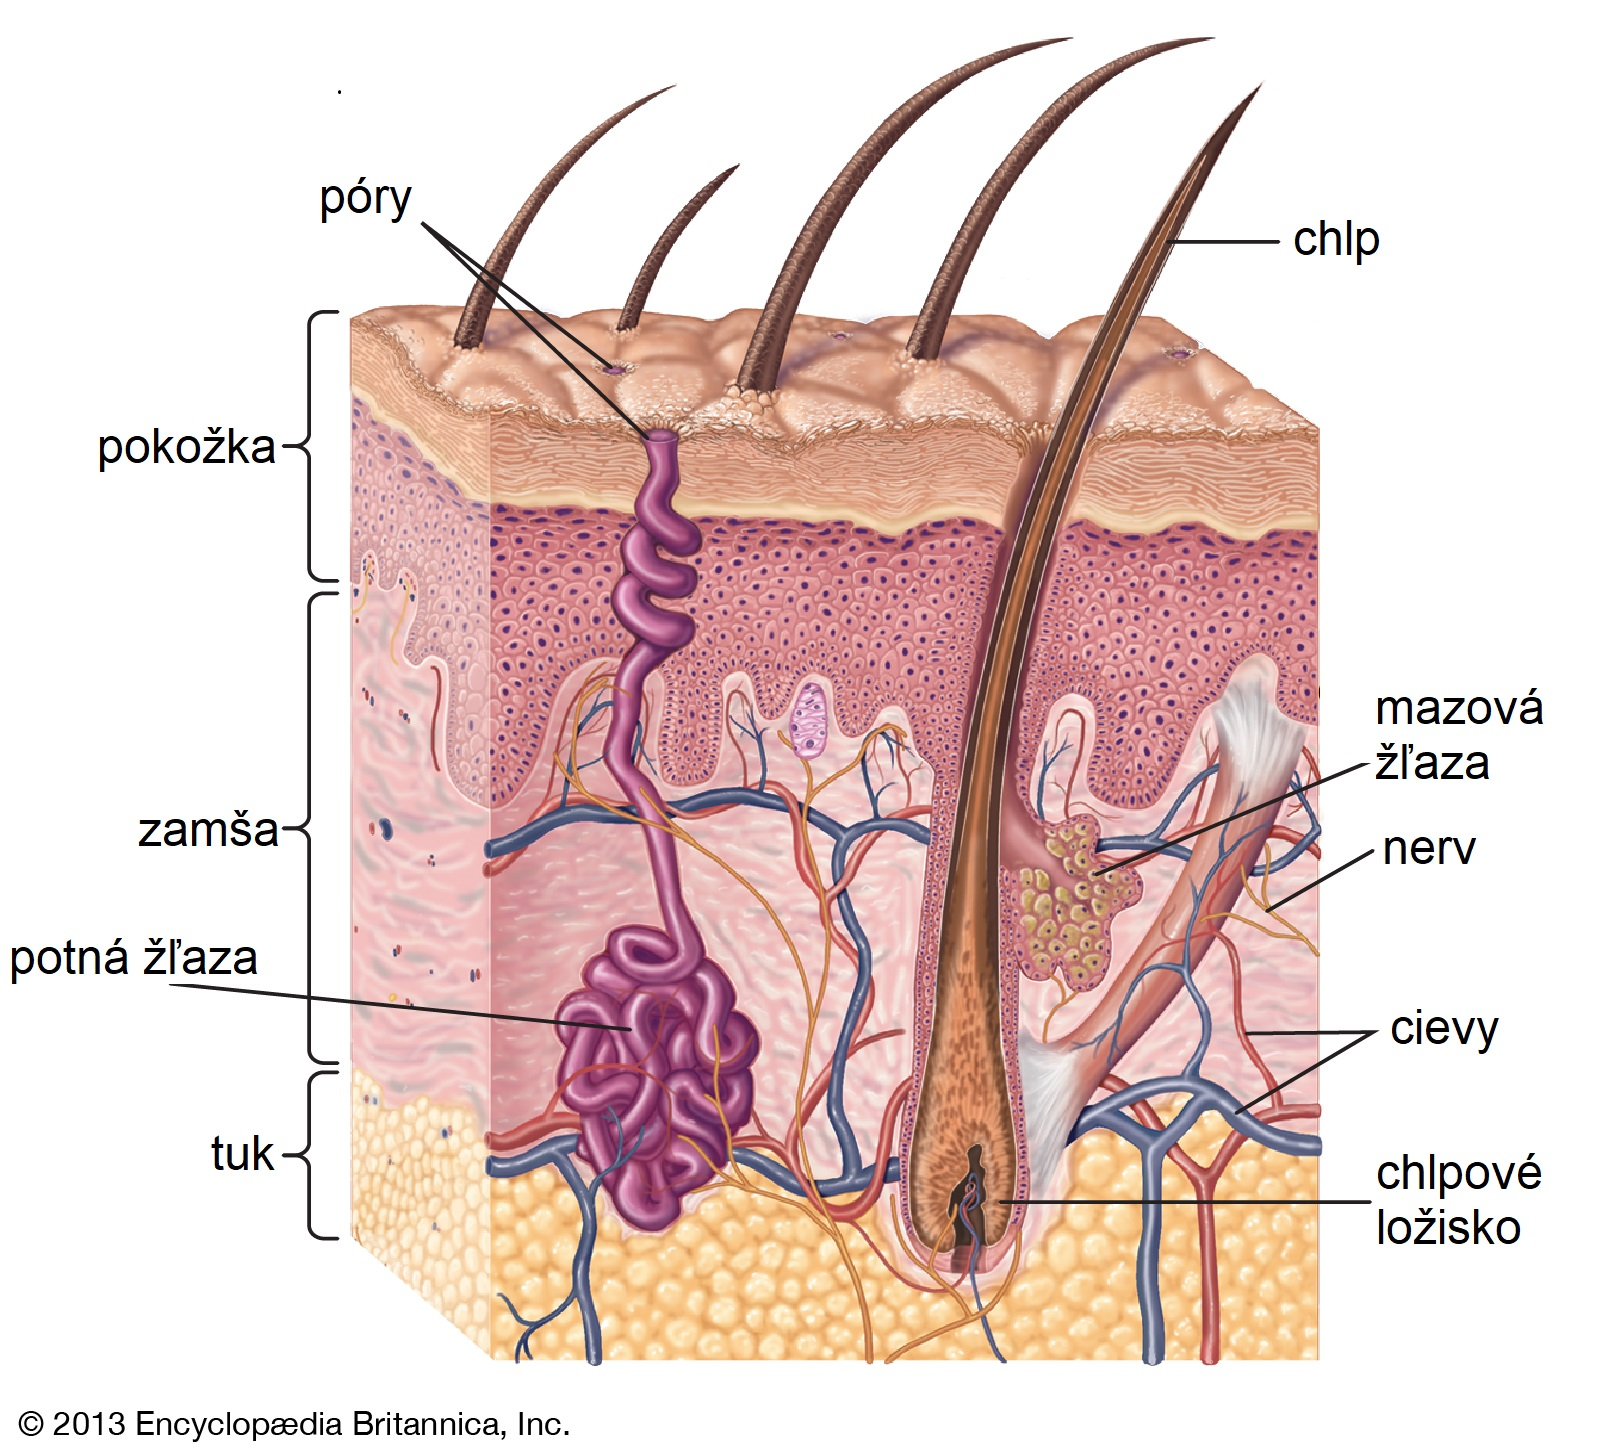
\includegraphics[scale=0.19]{fig/koza.jpg}
  \caption{Zloženie ľudskej kože. Zdroj \cite{Ebling2016}}
  \label{fig:koza}
\end{figure}

%%%%%%%%%%%%%%%%%%%%%%%%%%%%%%%%%%%%%%%%%%%%%%%%%%%%%%%%%%%%%%
\section{Kožná rana}
Kožná rana je definovaná ako narušenie kontinuity kožného povrchu a integrity organizmu, narušenie anatomickej štruktúry a funkcie kože spôsobené rôznymi príčinami zasahujúcimi rôzne hlboko do podkožných tkanív \cite{Hlinkova2015}.

Kožné rany je možné rozdeliť na jednoduché a komplikované. Jednoduché kožné rany zasahujú do pokožky, zamše a podkožného tuku. Komplikované rany narozdiel od jednoduchých prenikajú hlbšie a poškodzujú dôležité nervovo-cievne zväzky a orgány. Komplikované rany je ďalej možné rozdeliť na penetrujúce a nepenetrujúce. Penetrujúca rana preniká do teľnej dutiny. Nepenetrujúca rana naopak nepreniká do telesnej dutiny. U každej rany, či už jednoduchej, komplikovanej, penetrujúcej, alebo nepenetrujúcej určujeme a popisujeme vlastnosti, ktoré sú veľmi dôležité pri sledovaní procesu hojenia rany a voľby optimálnej liečby. Medzi takéto vlastnosti patrí \cite{pcCdSrbbhhlr5YcQ}:
\begin{itemize} 
\item lokalizácia rany
\item veľkosť rany
\item hĺbka rany
\item tvar rany
\item smer rany
\item okraje rany
\end{itemize}

%%%%%%%%%%%%%%%%%%%%%%%%%%%%%%%%%%%%%%%%%%%%%%%%%%%%%%%%%%%%%%
\section{Triedenie a typy rán}
Rany a poškodenia je možné deliť do niekoľko skupín podľa rôznych kritérií. Rany sa delia podľa ich priebehu, podľa rozsahu ich poškodenia, podľa množstva choroboplodných zárodkov, podľa spôsobu hojenia, podľa lokalizácie, podľa postihnutých štruktúr a mnoho iných delení, pričom najdôležitejšie delenia sú tie, ktoré sú ďalej popísané podrobnejšie \cite{Hlinkova2015}.

Rany podľa priebehu sa delia na:
\begin{itemize} 
\item \textbf{akútne rany -} vznikajú v zdravom kožnom tkanive. Hoja sa obvykle v krátkom čase a bez komplikácií.
\item \textbf{chronické rany -} trvajú dlhšie než 4 týždne, alebo to sú rany, ktoré vznikajú v zmenenom tkanive, a ktoré aj cez všetku odpovedajúcu liečbu nevykazujú známky hojenia.
\end{itemize}
Rany podľa rozsahu sa delia na:
\begin{itemize} 
\item \textbf{plošné rany -} odtrhnutie kože s podkožím
\item \textbf{povrchové rany -} poškodenia kožného krytu, alebo časti podkožia
\item \textbf{hlboké rany -} poškodenie až do podkožia
\end{itemize}
Rany podľa množstva choroboplodných zárodkov sa delia na:
\begin{itemize} 
\item \textbf{čisté rany -} neinfikované rany bez zárodkov a bez príznakov zápalu (chirurgický rez)
\item \textbf{čisté kontaminované rany -} rany bez dôkazu infekcie vzniknuté pri operácií orgánov dýchacieho, tráviaceho, pohlavného alebo močového ústrojenstva
\item \textbf{kontaminované rany -} penetrujúce traumatické rany, pri ktorých sú prítomné príznaky zápalu 
\item \textbf{infikované rany -} rany obsahujúce odumreté tkanivo s premnoženými mikroorgnizmami (rany vzniknuté po pohryznutí, poprípade zanedbané, alebo zastaralé rany)
\end{itemize}
Rany podľa spôsobu hojenia sa delia na:
\begin{itemize} 
\item \textbf{rany s primárnym hojením -} vďaka zlepeniu/zošitiu okrajov rany nevzniká nové spojivové tkanivo
\item \textbf{rany so sekundárnym hojením -} rana sa hojí novo tvoreným tkanivom
\end{itemize}

%%%%%%%%%%%%%%%%%%%%%%%%%%%%%%%%%%%%%%%%%%%%%%%%%%%%%%%%%%%%%%
\section{Príčiny rán}
Rany môžu vznikať pôsobením rôznych príčin, medzi ktoré patria vonkajšie, vnútorné príčiny alebo kombinácia týchto dvoch. Medzi vonkajšie príčiny patria rany rezné, sečné, tržné, rany spôsobené pohryznutím, bodné, strelné, zhmoždené, popáleniny, omrzliny, poleptaniny a rany spôsobené z ožiarenia. Medzi vnútorné príčiny patria cievne vredy dolných končatín, neuropatické vredy, preležaniny, rany pri nádorových ochoreniach, rany pri infekčných ochoreniach a rany pri imunitných poruchách. Vo všeobecnosti sa dajú príčiny vzniku rán rozdeliť do troch základných oblastí a to podľa toho, na akom základe vznikajú \cite{Hlinkova2015}:
\begin{itemize} 
\item lokálne poruchy výživy kože
\item lokálneho pôsobenia tlaku, cievneho poškodenia
\item systémového ochorenia (infekčného, nádorového, krvného...)
\end{itemize}

%%%%%%%%%%%%%%%%%%%%%%%%%%%%%%%%%%%%%%%%%%%%%%%%%%%%%%%%%%%%%%
\section{Chronické rany}
V kapitole Triedenie a typy rán boli rany rozdelené podľa priebehu na akútne a chronické. 

Akútne rany nie sú predmetom tejto práce, avšak pre celistvosť sú tu uvedené. Akútna rana je porušenie integrity tkaniva teľa vzniknuté v dôsledku fyzikálneho, mechanického, alebo termického poškodenia. Vznikajú v zdravom kožnom tkanive. Hoja sa obvykle v krátkom čase a bez komplikácií. Ich príčinou je väčšinou úraz, alebo chirurgický zákrok. Patria sem rany mechanické, traumatické, termické, chemické, aktinické, opary a pľuzgiere \cite{pcCdSrbbhhlr5YcQ}.

Chronická rana je sekundárne hojaca sa rana, ktorá sa musí uzavrieť pomocou výstavby nového tkaniva. Vzniká najčastejšie následkom lokálnych porúch vyživovania kože podmienených cievnym, alebo neurologickým ochorením, prípadne dlhodobým lokálnym pôsobením tlaku. Aj napriek adekvátnej liečbe sa takáto rana nezahojí skôr ako za 9 týždňov. Doba hojenia je spravidla dlhá a závisí na príčine a rozsahu poškodeného tkaniva. Chronické rany môžu vzniknúť aj z akútnych rán a to tak, že akútna rana je neadekvátne ošetrená, prípadne vznikne infekcia. Chronické rany sa taktiež objavujú v patologicky zmenených tkanivách. Medzi najčastejšie chronické rany patria bercové vredy, dekubity (preležaniny), diabetická noha, nádory s vredovým rozpadom, alebo komplikovane sa hojace pooperačné rany \cite{Hlinkova2015}.

\subsection{Bercové vredy}
Bercové vredy sú poškodením kožného krytu zasahujúce rôzne hlboko do podkožného tkaniva v oblasti členku. Nachádza sa najčastejšie v miestach medzi kolenom a členkom, hlavne v oblasti vnútorného členku.

Príčinou vzniku vredov býva drobné poranenie, alebo infekcia. Väčšina bercových vredov je žilného pôvodu a sú prejavom hromadenia krvi v dolných končatinách. Pri pretlaku v žilnom riečisku dochádza k žilnej nedostatočnosti. Žily na končatinách sa rozširujú, chlopne strácajú svoju správnu funkciu a prepúšťajú časť krvi naspäť. Prietok končatinami sa spomaľuje, tekutina z krvi v preplnených žilách prestupuje do podkožia, rozvíja sa opuch, ktorého následkom dochádza k poruche výživy kože. 

Prvým prejavom toho, že vzniká bercov vred je miestne začervenanie. Koža nad postihnutým miestom sa ztenčuje, je suchá, môže ju prekrývať šedivý ekzém a toto miesto je často dobre ohraničené s rovnými okrajmi. Bercove vredy bývajú rozsiahle, vlhké, skôr plytké a s povlečenou spodinou. Väčšinou sú sprevádzané rozsiahlym opuchom postihnutej oblasti a ďalšími kožnými zmenami. Okolie vredu vykazuje známky žilnej nedostatočnosti, hromadenie pigmentu, stráta ochlpenia. Bercové vredy sú často bolestivé \cite{pcCdSrbbhhlr5YcQ, Pokorna2012}.
\begin{figure}[h]
  \centering
  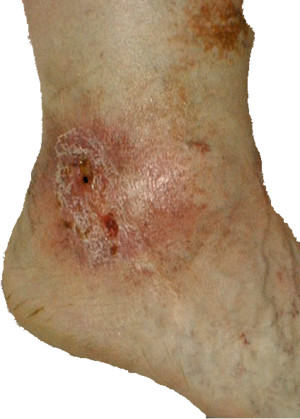
\includegraphics[scale=0.50]{fig/bercov-vred.png}
  \caption{Bercov vred žilného pôvodu. Zdroj \cite{BsyXZC783dJbfdc7}}
  \label{fig:bercov-vred}
\end{figure}

\subsection{Dekubity}
Dekubity, známe tiež ako preležaniny, sú rany spôsobené pôsobením lokálneho tlaku na kožu. Vznikajú v miestach dlhodobého kontaktu kože s podložkou. Sú typické pre chorých ľudí, ktorí sú dlhodobo pripútaní na lôžko.

Príčinou vzniku preleženín je to, že v miestach neustáleho kontaktu a tlaku dochádza k uzatvoreniu drobných ciev. Tkanivo je zle zásobované živinami a kyslíkom, a tak dochádza k ich postupnému odumieraniu. Rozsah odumretia tkaniva závisí na vzájomnom pôsobení niekoľkých faktorov. Konkrétne závisí na intenzite tlaku, doby pôsobenia tlaku, odolnosti organizmu voči tlaku, celkového stavu postihnutia a vplyvov vonkajšieho prostredia. Preležaniny sa objavujú pomerne rýchlo, v ojedinelých prípadoch už po niekoľkých hodinách.

K miestam najnáchylnejším k vzniku dekubitov patria oblasti s malou vrstvou tukového a svalového tkaniva, kde z vonka pôsobí tlak priamo na kosti. Medzi takéto oblasti patrí oblasť nad krížovou kosťou, päty, sedacie kosti, oblasť nad veľkými výčnelkami stehennej kosti a vonkajšie členky. Avšak napriek tomu sa môžu vytvoriť kdekoľvek na tele. Vývoj preležanín prebieha v niekoľkých štádiách. Prvým prejavom je začervenanie, bolestivosť a opuchnutie kože. Nasleduje pľuzgier, alebo povrchový vred zasahujúci do pokožky a zamše, v okolí sa rozvíja zápal. Posledným štádiom je odumretie tkaniva. Nedostatočne liečená preležanina sa ďalej prehlbuje, odumreté tkanivo sa topí, hnilobne páchne a zvyšky tkaniva majú žltozelenú farbu \cite{pcCdSrbbhhlr5YcQ, Hlinkova2015}.
\begin{figure}[h]
  \centering
  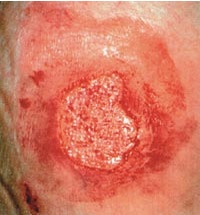
\includegraphics[scale=1]{fig/dekubit.png}
  \caption{Preležanina v druhom štádií. Zdroj \cite{Vilimovsky2015}}
  \label{fig:dekubit}
\end{figure}

\subsection{Diabetická noha}
Syndrómom diabetickej nohy sa označujú defekty dolných končatín, spôsobené postihnutím ciev a nervov. Ide o komplikáciu ochorenia cukrovky.

Medzi 2 hlavné príčiny vzniku tohoto syndrómu sa dá označiť diabetická neuropatia a ischemická choroba dolných končatín. Diabetickou neuropatiou je myslená dlhodobo zvýšená hladina cukru v krvi, ktorá poškodzuje funkciu a štruktúru periférnych nervov. Postihnutie sa týka všetkých typov nervových vlákien. Obmedzenie, alebo strata funkcie ma priamy dopad na nohu:
\begin{itemize}
\item \textbf{senzorická neuropatia -} vedie k strate citlivosti na bolesť, teplotu, vibrácie, tlak a polohocit.
\item \textbf{motorická neuropatia -} vedie k oslabeniu a skráteniu svalstva a vzniku otlakov.
\item \textbf{vegetatívna neuropatia -} vedie k zníženému poteniu kože, strate jej pružnosti a tým k vyššiemu riziku prasklín.
\end{itemize}

Za ischemickú chorobu dolných končatín sa označuje ochorenie tepien, ktoré spôsobuje nedostatočné prekrvenie dolných končatín. Hlavnou príčinou ochorenia je ateroskleróza, ktorá má za následok zúženie, alebo úplný uzáver tepien a obmedzenie prítoku krvi. Okrem veľkých ciev sú v prípade diabetickej nohy postihnuté aj jemné vlásočnice. Takto nedostatočne prekrvené tkanivo je náchylné k poraneniu a vykazuje zlú hojivosť.

Medzi prejavy diabetickej nohy v kľude patria nepríjemné pálčivé bolesti, brnenie, alebo mravenčenie končatín. Pri chôdzi sa zase prejavuje pocitom stiahnutia okolo členkov. Koža nohy je suchá a šúpe sa. Svaly lýtok sú oslabené, ochlpenie je preriedené, alebo chýba úplne. Pri nedokrvení končatín sa môže objaviť aj bolesť, ale nie je to pravidlom. Najčastejším miestom vzniku sú členky, priehlavok, päta a prsty. Medzi ďalšie prejavy patria praskliny, pľuzgiere a odreniny, ktoré keď sa neliečia, tak sa rozširujú, poprípade sa do toho pridá infekcia \cite{pcCdSrbbhhlr5YcQ, Pokorna2012}.
\begin{figure}[h]
  \centering
  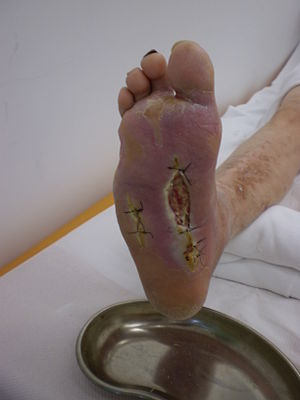
\includegraphics[scale=2]{fig/diabeticka-noha.jpg}
  \caption{Syndróm diabetickej nohy. Zdroj \cite{uGOum7N9LzIGa5X2}}
  \label{fig:diabeticka-noha}
\end{figure}

\subsection{Maligne rany}
Nehojace sa rany a kožné defekty, ktoré vznikajú pri nádorových ochoreniach sa nazývajú maligne rany. Vyskytujú sa najčastejšie u pacientov s pokročilými nádorovými ochoreniami. Vznikajú v súvislosti so spinocelulárnym karcinonom, bazocelulárnym karcinonom, malignym melanonom, alebo zhubným nádorom (pŕs, hlavy, krku,...).

Príčiny vzniku týchto rán sa dajú zhrnúť do 3 oblastí: Primárne kožný nádor, prerastanie nádoru mäkkých tkanív do kože a kožné metastázy nádoru. Rastom nádoru dochádza k narušeniu kožných kapilár a lymfatických ciev a k útlaku okolných tkanív. To vedie k obmedzeniu prísunu živín a vzniku nekrózy.

Na začiatku sa v koži najčastejšie objaví zatvrdnutie, ktoré je nasledované začervenaním a rozvojom nekrózy. Maligne rany doprevádza prevažne krvácanie, sekrécia rany, nepríjemný zápach, bolesť a svrbenie okolia rany \cite{pcCdSrbbhhlr5YcQ, Hlinkova2015}.
\begin{figure}[h]
  \centering
  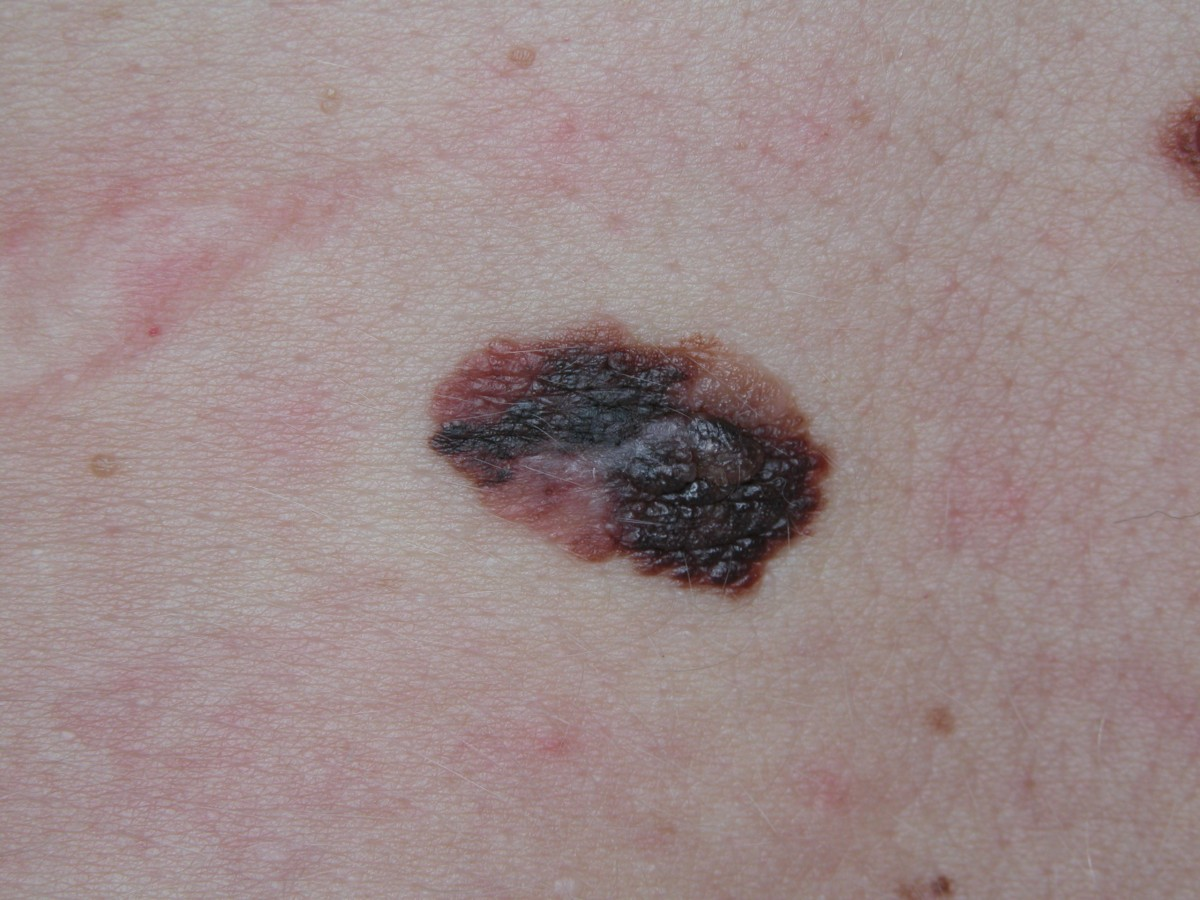
\includegraphics[scale=0.20]{fig/maligna-rana.png}
  \caption{Malígny melanóm. Zdroj \cite{Svehlik2012}}
  \label{fig:maligny-melanom}
\end{figure}

\subsection{Pooperačné rany}
Už ako samotný názov napovedá, ide o rany, ktoré vznikli v rámci operačného výkonu. Spôsob a vzhľad obnovenia integrity kože nerušenej pri operačnom výkone záleží na chirurgovi, ktorý zákrok vykonával. O tom, akým spôsobom sa ale bude rana hojiť, a ako bude vypadať výsledná jazva, rozhoduje celá rada ďalších faktorov.

Príčinou komplikovaného hojenia operačnej rany je väčšinou infekcia. Kontaminácia rany mikroorganizmami môže byť spôsobená samotným charakterom operácie, avšak ale aj porušením aseptických pravidiel, alebo následným preväzom. Väčšina ranných infekcií je avšak spôsobená mikroorganizmami, ktoré boli v organizme prítomné už pred vznikom infekcie. K najčastejším pôvodcom patria stafylokoky, streptokoky, klebsiely, kvasiny, alebo pseudomonády.

Prejavom takýchto rán je v rannom štádiu opuch a začervenanie rany a jej okolia. Ide o prejav zápalu, ktorým sa organizmus bráni pred poškodením. Tieto prejavy sú v rôznej miere zastúpené pri všetkých operačných ranách. Až prítomnosť hnisu je známkou infekcie. Infekcia sa prajavuje tak, že žltá, alebo nazelenalá tekutina sa hromadí v rane a zväčšuje jej objem, alebo dokonca vyteká. Rana sa potom následne rozpadá, jej stehy sú povlečené a priľahlé rany nekrotické. Infekcia zasahuje do rôznej hĺbky. V niektorých prípadoch sa obmedzuje iba na kožu a podkožie, v iných zase postihuje všetky vrstvy rany \cite{pcCdSrbbhhlr5YcQ}.
\begin{figure}[h]
  \centering
  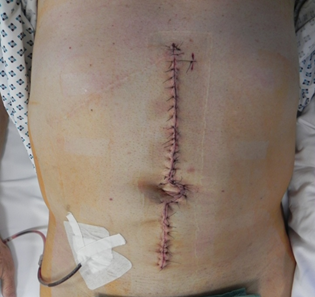
\includegraphics[scale=1]{fig/pooperacna-rana.png}
  \caption{Operačná rana po klasickej laparotómii. Zdroj \cite{XUKYT8x1LmEzzkqO}}
  \label{fig:pooperacna-rana}
\end{figure}

\section{Hojenie rán}
Hojenie je fyziologický proces, pri ktorom dochádza k obnove porušenej štruktúry a funkcie kože. Je to reparačný proces, pri ktorom je poškodené tkanivo nahradené väzivovým tkanivom, ktoré sa postupne mení na jazvu. Hojenie rany ovplyvňuje niekoľǩo faktorov, ktoré sa dajú rozdeliť na lokálne a celkové. Medzi lokálne faktory patrí porucha krvného zásobovania, stav okolitého tkaniva, pôsobenie tlaku, prítomnosť infekcie, nevhodné šicie materiály a technika, pohyb v rane, teplota, pH, dehydratácia a opuch. Medzi celkové faktory ovplyvňujúce hojenie patrí vek, celkový zdravotný stav pacienta, stav imunitného systému, anémia, strata krvi, podvýživa, nedostatok bielkovín, vplyv liekov, imobilita a psychický stav \cite{pcCdSrbbhhlr5YcQ, Pokorna2012}.

Hojenie rán prebieha v niekoľkých vzájomne prelínajúcich sa, časovo prekrývajúcich sa a na seba nadväzujúcih fází a prebieha odlišne pri akútnych ranách a chronických ranách. Hojenie chronických rán je o niečo komplikovanejšie než hojenie akútnych rán. Tieto rany sa zaceľujú výstavbou nového tkaniva. Doba ich hojenia je veľmi zdĺhavá a závisí na rozsahu poškodenia tkaniva. Hojenie prebieha v 3 hlavných fázach \cite{Pokorna2012}:
\begin{enumerate}
\item \textbf{fáza zápalu -} je charakteristická snahou odstrániť všetky nežiaduce zložky, zaistiť odlúčenie poškodených a odumretých tkanív. Liečba je zameraná na podporu samo-čistiacich procesov v kombinácií spolu s chirurgickým ošetrením.
\item \textbf{fáza granulácie -} po vyčistení z fáze 1 sú vytvorené podmienky pre rast a delenie nových buniek a vzniká granulačné tkanivo, ktoré je podkladom pre proces epitelizácie.
\item \textbf{fáza epitelizácie -} finálna etapa, v ktorej dochádza k deleniu a pohybu kožných buniek. Z okrajov rany prerastá epitel a pokrýva granulačné tkanivo novo-vytvorenou kožou.
\end{enumerate}

Hodnotenie hojenia rany prebieha podľa niekoľkých základných vlastností. Medzi tieto vlastnosti patrí príčina vzniku, vek rany, veľkosť, okraje, lokalizácia, hĺbka, vzhľad spodiny, bolestivosť, prítomnosť infekcie, množstvo sekrécie, zápach, okolie rany a súčasná a minulá lokálna terapia. Informácie boli prebrané z \cite{pcCdSrbbhhlr5YcQ}.

\chapter{Analýza a návrh riešenia}
\label{chap:analyza-navrh-riesenia}
V tejto kapitole je popísaný postup analýzy a návrhu riešenia tejto diplomovej práce. Najprv je popísaná analýza požiadaviek na výslednú aplikáciu a jej primárnu funkcionalitu. Ďalej je popísaný návrh samotnej mobilnej aplikácie, kde sú predstavené prípady užitia a použitia aplikácie, ako aj základný návrh grafického užívateľského rozhrania. Potom nasleduje návrh databáze, ktorý bol realizovaný pomocou ER diagramu. Posledná kapitola pojednáva o návrhu aplikačného rozhrania vychádzajúceho z princípov RESTu.

%%%%%%%%%%%%%%%%%%%%%%%%%%%%%%%%%%%%%%%%%%%%%%%%%%%%%%%%%%%%%%
\section{Analýza požiadaviek}
Analýza požiadaviek čiastočne vychádza z kapitoly \ref{chap:teoreticky-rozbor}, v ktorej boli popísané dôležité teoretické znalosti a zároveň vychádza z informácií poskytnutých Fakultnou nemocnicou Brno a jej požiadavok. Podľa týchto informácií a požiadavok by malo ísť o aplikáciu určenú pre platformy Android, iOS a Windows Mobile, ktorá by mala umožňovať vyfotografovať chronickú ranu, primárne preležaninu, spolu s nejakou mierkou. Mierka by mala byť buď pero, alebo prst zdravotnej sestry, prípadne ošetrujúceho lekára a mal by byť nastaviteľný jeho rozmer. Aplikácia by mala byť schopná následne odfotografovanú ranu detekovať, lokalizovať a spočítať plošný rozmer cieľovej plochy, napríklad v milimetroch štvorcových alebo inej miere. V aplikácií by mala byť možnosť prihlásenia užívateľa pomocou sociálnych sietí, ako napríklad Facebook alebo Google+. Ďalej by mal mať užívateľ možnosť svoje snímky pomenovať, porovnať s minulými snímkami, mať možnosť tlače týchto snímok a prípadne ich ukladať na vzdialené úložisko, aby k nim mal prístup aj z iného zariadenia ako je aktuálne používané. Aplikácia by mala byť primárne cielená na zdravotné sestry, poprípade ošetrovateľov starajúcich sa o chronické rany a pomáhať im so sledovaním vývoja rán v čase. 

Z vyššie uvedeného vyplýva, že aplikácia by mala byť dostupná na väčšinu platforiem, aj keď nie v rámci tejto diplomovej práce, ale predovšetkým v rámci dlhšieho časového horizontu vývoja. Z tohoto dôvody bolo usúdené, že by bolo dobré, ak by sa vytvorila hybridná aplikácia, ktorú stačí naprogramovať raz a už iba s drobnými úpravami je ju možné potom publikovať na väčšine dostupných platforiem. Keďže samotné spracovanie obrazu má v hybridných aplikáciách, webových aplikáciách a celkovo v Javasciptovom svete mizivú podporu, tak by spracovanie obrazu (konkrétne detekcia, lokalizácia a určenie plochy) nastávalo vzdialene na servery. Kvôli tomu bolo rozhodnuté, že programová realizácia by mala byť rozdelená na niekoľko logických celkov, ktorých existencia by bola navzájom od seba nezávislá. Mala by sa skladať zo samotnej mobilnej aplikácie, ktorá môže byť chápaná aj ako klientská časť realizácie, keďže ju bude vidieť každý používateľ aplikácie. Ďalej by išlo o databázovú časť, do ktorej by sa ukladali samotné dáta a potrebné informácie spojené s jednotlivými ranami, užívateľmi a snímkami. A nakoniec ako spojovník medzi týmito 2 časťami by figurovalo aplikačné rozhranie vzdialené na serverovej časti, ktoré by komunikovalo s klientskými aplikáciami, ukladalo a získavalo dáta z databáze, umožňovalo autorizáciu a autentifikáciu používateľov, a spracovávalo snímky rán.

%%%%%%%%%%%%%%%%%%%%%%%%%%%%%%%%%%%%%%%%%%%%%%%%%%%%%%%%%%%%%%
\section{Návrh aplikácie}
Návrh samotnej aplikácie bol vypracovaný s rešpektom k analýze požiadaviek. Bolo nutné premyslieť, čoho všetkého by mala byť daná aplikácia schopná, ako by mala plniť svoju úlohu čo najlepšie a čo by mal byť jej hlavný cieľ okrem samotnej detekcie, lokalizácie a určenia plochy chronickej rany. Aplikácia by nemala byť robustným informačným systémom, skôr iba čo možno najjednoduchšie poňatou aplikáciou, zbytočne nezaťažujúcou užívateľa, ale ponúkajúcou dostatočné možnosti pre pomoc so sledovaním chronických rán. Samotný návrh aplikácie bol rozdelený na 2 podkapitoly, a to na návrh funkcionality, alebo toho, čo by mal byť užívateľ schopný vykonávať, a do návrhu užívateľského rozhrania.

\subsection{Návrh funkcionality}
Návrh funkcionality aplikácie bol spracovaný pomocou Diagramu prípadov užitia (Use Case Diagramu), ďalej iba UCD. UCD zobrazuje chovanie systému z pohľadu užívateľa. Jeho účelom je popísať funkcionalitu systému, presnejšie čo presne sa od samotného systému očakáva. Diagram zobrazuje to, čoho má systém, v tomto prípade aplikácia, byť schopný ale už nehovorí o tom, ako sa to bude vykonávať. Diagram je zložený z prípadov užitia (Use Case), aktérov (Actor) a vzťahov medzi nimi. Prípad užitia je sada niekoľkých akcií, ktoré vedú k dosiahnutiu určitého cieľa. Aktér je rola, ktorá komunikuje s jednotlivými prípadmi užitia. UCD je teda v podstate diagram, ktorý zobrazuje všetko to, čo daná užívateľská rola, alebo konkrétny užívateľ môže v systéme vykonávať.

Jedinou rolou v aplikácií, tvorenej v rámci tejto diplomovej práce, je rola všeobecného užívateľa, ktorým je väčšinou zdravotná sestra, lekár, alebo iný ošetrovateľ starajúci sa o chronickú ranu. Každý užívateľ, ktorý si zapne aplikáciou, by sa mal automaticky stať roľou ošetrovateľa. Ošetrovateľ by mal mať možnosť zobraziť si zoznam liečení. Tento zoznam by mal obsahovať liečenia, ktoré aktuálne prebiehajú a sú v určitom štádií, ale zároveň aj liečenia, ktoré už nie sú aktívne pozorované a považujú sa za ukončené. Tento zoznam by mal byť filtrovateľný minimálne podľa stavu liečby a malo by sa v ňom zároveň dať vyhľadávať podľa mena liečeného pacienta. Ďalej by mal byť ošetrovateľ schopný vytvoriť nové liečenie, zobraziť detail už existujúceho liečenia a mať možnosť meniť toto liečenie. Okrem toho by mal mať možnosť zobraziť graf postupu liečenia, konkrétne graf zmeny veľkosti detekovanej plochy chronickej rany a mať možnosť tieto výsledky uložiť do PDF formátu, poprípade vytlačiť. Pre každé liečenie by mal mať možnosť ošetrovateľ potom zobraziť zoznám vytvorených snímkov rán, urobiť novú snímku, zobraziť detail existujúcej snímky, zmeniť snímku a prípadne ju odstrániť. Dôležitým aspektom v aplikácií by mala byť mierka, ktorej význam bude vysvetlený v ďalších kapitolách. Užívateľ aplikácie by mal mať možnosť zobraziť existujúce mierky, tak ako ich aj meniť a odstraňovať. Mierky by sa mali dať tiež pridávať a malo by sa dať voliť, ktorá bude nastavená ako východzia. Celý Diagram prípadov užitia je možné vidieť na obrázku \ref{fig:usecase}.
\begin{figure}[h]
      \centering
      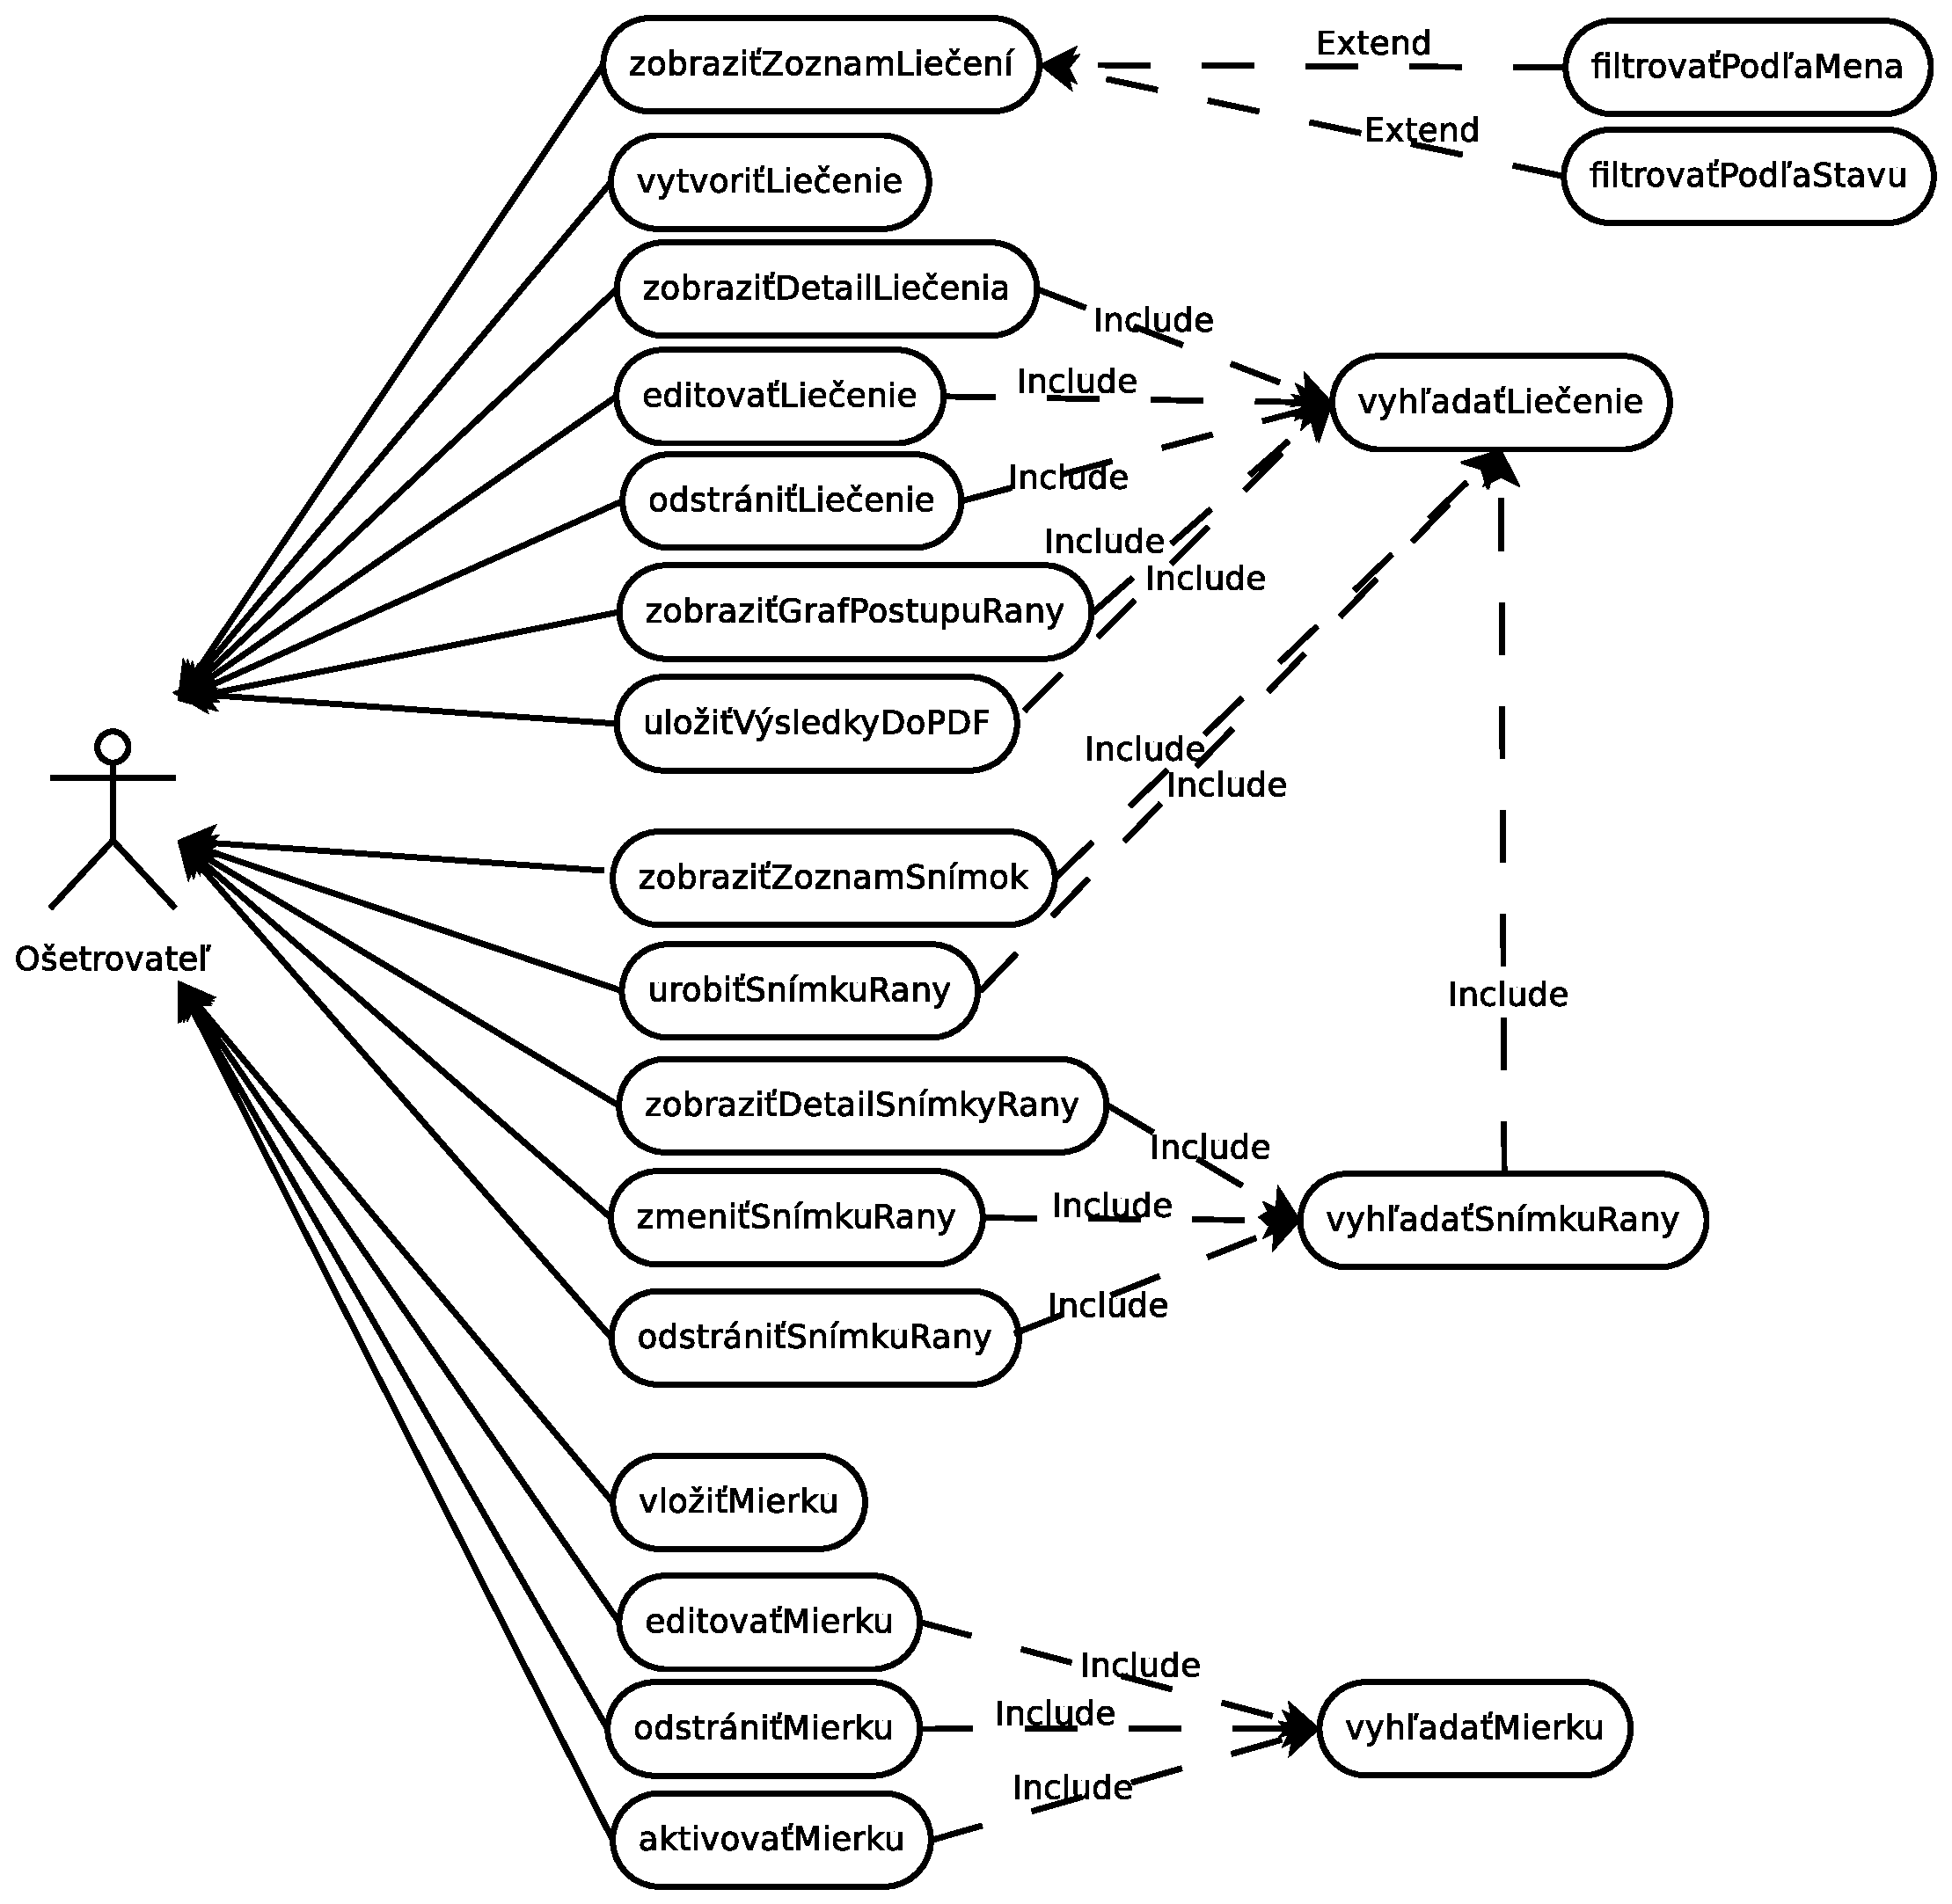
\includegraphics[scale=0.420]{fig/use-case.eps}
      \caption{Diagram prípadov užitia užívateľa aplikácie}
      \label{fig:usecase}
\end{figure}

\subsection{Návrh grafického užívateľského rozhrania}
Grafické užívateľské rozhranie bolo navrhnuté najprv na papier a potom pre lepšie predstavenie boli tieto náčrty prevedené do digitálnej podoby programom Wireframe Sketcher.

Prvá obrazovka, ktorá bola navrhnutá je obrazovka prihlásenia. Na túto obrazovku by sa mal dostať užívateľ vtedy, keď nie je prihlásený. Typicky sa tak deje pri prvom spustení aplikácie. Pri ďalších spusteniach by si aplikácia mala zapamätať užívateľa a prihlasovať ho už automaticky. Prihlásenie do aplikácie by malo byť povinné a v prípade, že nie je užívateľ prihlásený tak by sa nemalo dať pokračovať ďalej. Na tejto obrazovke by sa malo nachádzať iba tlačidlo na prihlásenie cez nejakú sociálnu sieť, či už Facebook, Google+ alebo obidvoje. Okrem samotného tlačidla by mal byť prítomný aj nejaký vysvetľujúci text. Návrh prihlasovacej obrazovky je možné vidieť na obrázku \ref{fig:mockup1}.
\begin{figure}[h]
      \centering
      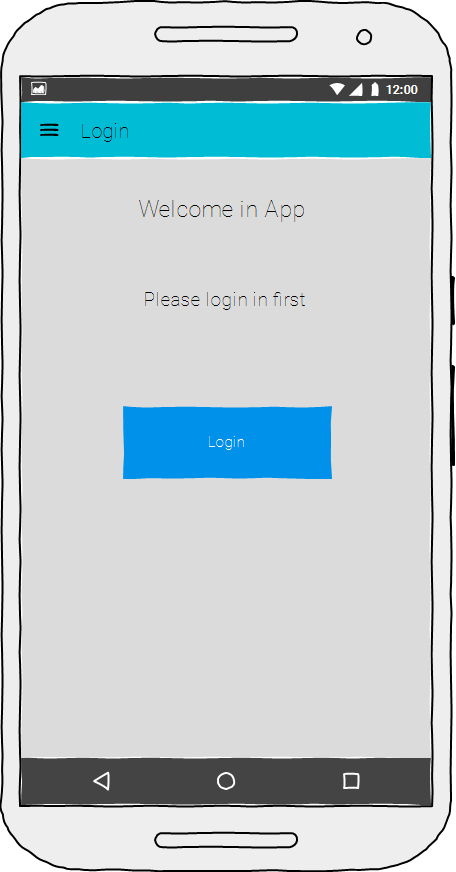
\includegraphics[scale=0.45]{fig/mockup1.png}
      \caption{Obrazovka prihlásenia}
      \label{fig:mockup1}
\end{figure}

Po prihlásení do systému aplikácie by mal mať užívateľ zobrazený zoznam všetkých liečení, mala by tam existovať možnosť filtrácie a vyhľadávania umiestneného na panely aplikácie a vo vyskakovacom menu. Každý prvok zoznamu by mal mať zobrazené svoje meno liečenia, meno liečeného pacienta a posledný dátum kontroly (lepšie povedané posledný dátum fotografovania rany). V pravom dolnom rohy by malo byť plávajúce tlačidlo na pridávanie liečení. Návrh je možné vidieť na obrázku \ref{fig:mockup4}. 

Po výbere konkrétnej položky by mal byť užívateľ prenesený na obrazovku detailu liečby. V tejto obrazovke by mal mať možnosť vidieť všetky informácie o liečbe (ako napríklad meno pacienta, narodenie pacienta, stav liečby, stav rany...), graf znázorňujúci vývoj rany v čase a zoznam odfotografovaných rán obsahujúci ich mená a dátumy zachytenia snímky. V pravom dolnom rohy by malo byť plávajúce tlačidlo na odfotografovanie rany. Liečbu by bolo možné na tejto obrazovke editovať, poprípade vymazať výberom z vyskakovacieho menu umiestneného v pravom hornom rohu. Mockup je znázornený na obrázku \ref{fig:mockup5}.
\begin{figure}[h]
   \begin{minipage}{0.48\textwidth}
     \centering
     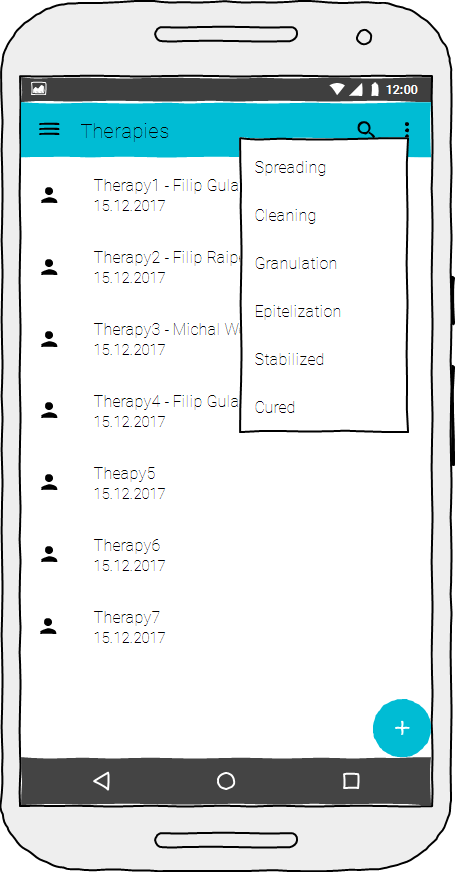
\includegraphics[scale=0.45]{fig/mockup4.png}
      \caption{Obrazovka zoznamu liečení}
      \label{fig:mockup4}
   \end{minipage}\hfill
   \begin {minipage}{0.48\textwidth}
     \centering
     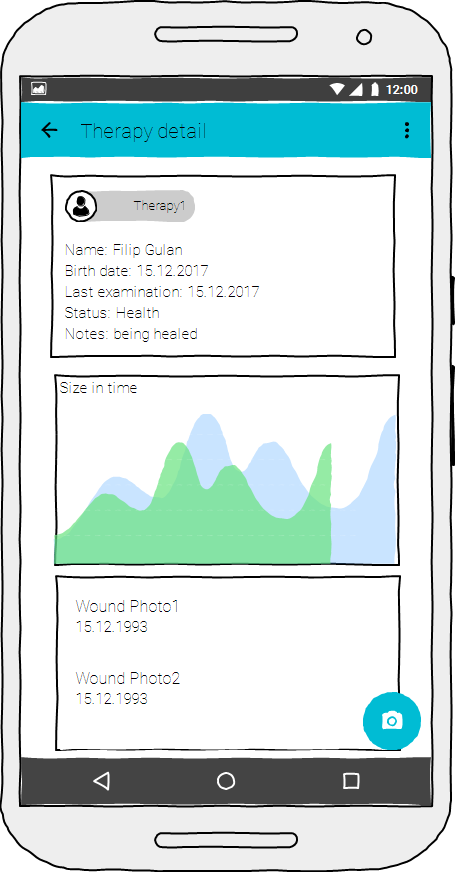
\includegraphics[scale=0.45]{fig/mockup5.png}
      \caption{Obrazovka detailu liečenia}
      \label{fig:mockup5}
   \end{minipage}
\end{figure}

V prípade, že sa užívateľ rozhodne fotiť ranu, tak by sa mala aktivovať aplikácia kamera, pomocou ktorej by urobil fotku a táto fotografia by bola následne prenesená na server pre detekciu, lokalizáciu a určenie plochy rany. Po tejto detekcií by bola užívateľovi vrátená upravená fotka zo serveru obsahujúca ohraničenie rany a bola by mu zobrazená ako náhľad, podľa ktorého by sa rozhodol, či mu vyhovuje a chce ju zachovať, alebo či chce urobiť vhodnejší snímok rany. Táto obrazovka náhľadu nasnímanej, detekovanej a lokalizovanej rany je možné vidieť na obrázku \ref{fig:mockup6}. 

V prípade, že sa užívateľ rozhodne, že mu odfotografovaný snímok vyhovuje, tak bude prenesený na obrazovku detailu rany. Na tejto obrazovke by sa mali nachádzať základné informácie o aktuálnom snímku rany (ako napríklad meno rany, vypočítaná veľkosť, dátum vykonania snímania a poznámka) a samotná snímka znázorňujúca ranu s jej ohraničením. Na túto obrazovku by sa mal užívateľ dostať aj keď si v detaile liečby vyberie danú konkrétnu fotku rany. Návrh je možné vidieť na obrázku \ref{fig:mockup7}.
\begin{figure}[h]
   \begin{minipage}{0.48\textwidth}
     \centering
     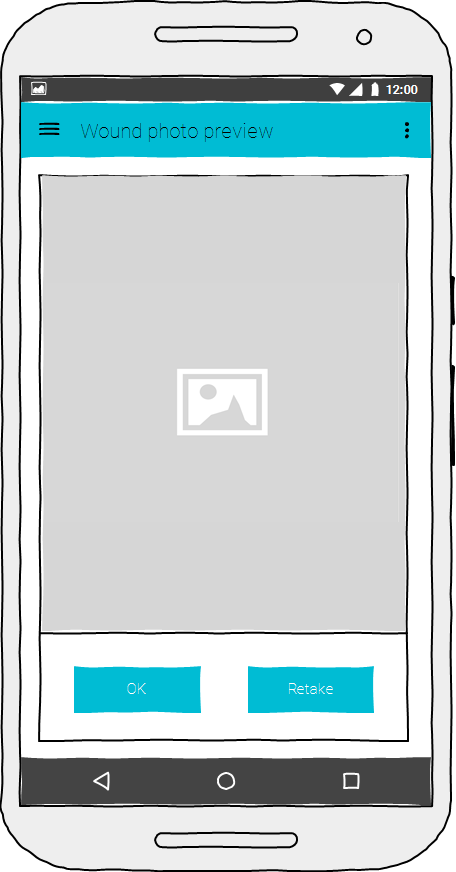
\includegraphics[scale=0.45]{fig/mockup6.png}
      \caption{Obrazovka náhľadu práve získanej a detekovanej rany}
      \label{fig:mockup6}
   \end{minipage}\hfill
   \begin {minipage}{0.48\textwidth}
     \centering
     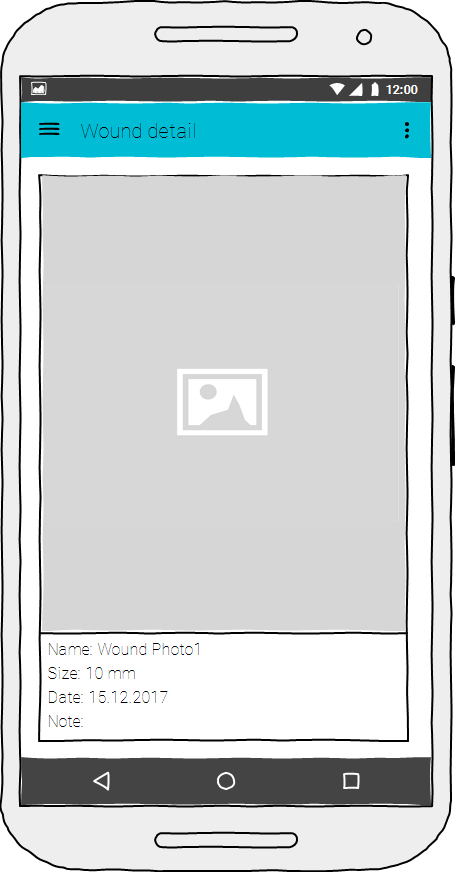
\includegraphics[scale=0.45]{fig/mockup7.png}
      \caption{Obrazovka detailu vyfotenej rany}
      \label{fig:mockup7}
   \end{minipage}
\end{figure}

Obrázok \ref{fig:mockup2} zobrazuje návrh globálneho menu, ktoré by malo byť dostupné z každej obrazovky. Toto menu by sa malo dať otvoriť z vrchného panelu aplikácie. Malo by obsahovať základné informácie o aktuálne prihlásenom užívateľovi, užívateľ by sa tu mal mať možnosť odhlásiť a mala by tu byť možnosť sa z tohoto menu dostať na obrazovku nastavení.
	
Na obrazovke nastavení zobrazenej na obrázku \ref{fig:mockup3} by sa mali dať spravovať predovšetkým jednotlivé mierky. Mali by sa tu dať pridávať, editovať a vymazávať pomocou kontextového okna. Zároveň by mala byť prítomná možnosť výberu mierky, ktorá sa aplikuje ako východzia.
\begin{figure}[h]
   \begin{minipage}{0.48\textwidth}
     \centering
     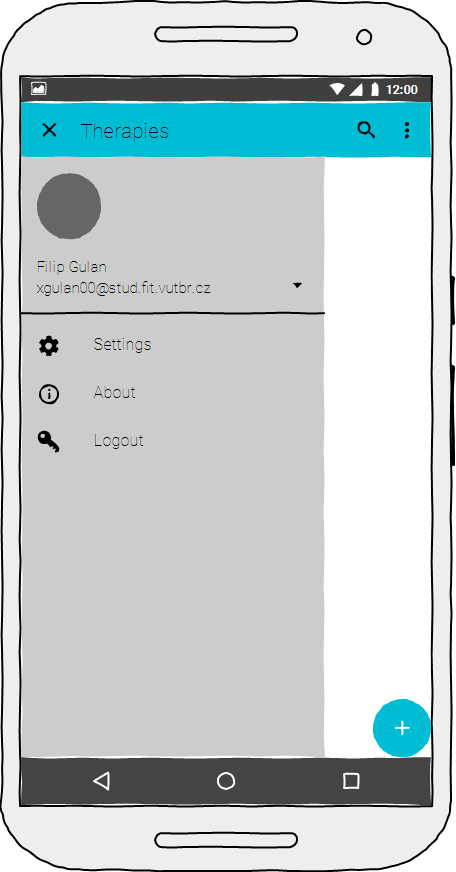
\includegraphics[scale=0.45]{fig/mockup2.png}
      \caption{Globálne menu}
      \label{fig:mockup2}
   \end{minipage}\hfill
   \begin {minipage}{0.48\textwidth}
     \centering
     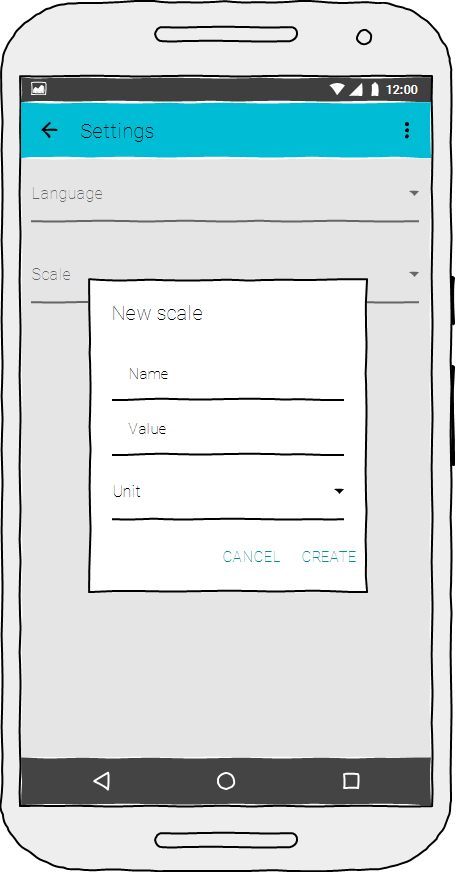
\includegraphics[scale=0.45]{fig/mockup3.png}
      \caption{Obrazovka nastavení a pridávanie mierky}
      \label{fig:mockup3}
   \end{minipage}
\end{figure}
\newpage

%%%%%%%%%%%%%%%%%%%%%%%%%%%%%%%%%%%%%%%%%%%%%%%%%%%%%%%%%%%%%%
\section{Návrh databáze}
Návrh databáze bol spracovaný pomocou Entity Relationship diagramu, ďalej iba ER diagram, s Unified modeling notáciou. Tento diagram sa používa v softwarovon inžinierstve pre konceptuálne a abstraktné znázornenie dát. Pri modelovaní ER diagramu vzniká jeden z typov konceptuálnych, alebo schematických dátových modelov systému a požiadavok naň z hora dole. V prípade, že sa jedná o návrh informačného systému založeného na databáze a aplikácia tejto diplomovej práce môže byť chápaná ako jednoduchý informačný systém, tak sa tento konceptuálny model v neskoršej fázy mapuje na logický dátový model a ten ďalej na fyzický dátový model.

Návrh využíva informácie  z predchádzajúcej kapitoly o Návrhu aplikácie a samotné návrhy spolu úzko súvisia, keďže funkcionalita pracuje s dátami, ktoré sa získavajú z databáze a zároveň sa do nej ukladajú. Informácie sú tu však podané mierne odlišne, tak aby z nich bolo možné namodelovať ER diagram a uvedomiť si vzťahy medzi jednotlivými entitami. Jednou z hlavných entít figurujúca v tomto databázovom návrhu je liečenie. Liečenie obsahuje svoj názov, aktuálny stav priebehu (ako napríklad dokončené, prebiehajúce, alebo iné). V každom liečení je vždy zapojený jeden konkrétny pacient. A každé liečenie prebieha vždy pod dohľadom jedného konkrétneho ošetrovateľa. Entita pacient obsahuje svoje meno, priezvisko a dátum narodenia. Okrem toho, že pacient podlieha jednému liečeniu, ako už bolo spomenuté, tak každý pacient má jednu ranu, ktorá ho trápi. Táto rana v sebe obsahuje svoj typ, príčinu rany, lokalizáciu a smer rany. Tieto 3 entitné množiny (terapia, pacient a rana) sú modelované ako slabé, z toho dôvodu, že vo výsledku budú brané ako jeden databázový záznam a v diagrame sú oddelené iba pre prehľadnosť návrhu. Nepredpokladá sa, že bude existovať X pacientov s X ranami. Skôr sa predpokladá jeden pacient, na ktorom bude sledovaná jedna rana. A ak by sa náhodou našiel pacient s viac ranami, tak sa iba pridá ďalšie liečenie, čo síce bude znamenať miernu redundanciu dát, ale vo výsledku bude aplikácia jednoduchšia na užívateľské rozhranie, keďže sa nebude musieť vždy vyberať zo zoznamu pacientov, poprípade pridávať nových do tohoto zoznamu. Každá rana môže obsahovať niekoľko svojich snímok a každá snímka patrí práve jednej rane. Každá táto snímka obsahuje svoj názov, veľkosť, dátum snímania, poznámku v prípade potreby. Ďalej snímka obsahuje či je aktuálne rana bolestivá, či zapácha, či sa na nej nachádza sekrét, či obsahuje infekciu a aké sú jej okraje. Každý tento snímok používa vždy jednu konkrétnu mierku a je sledovaná jedným konkrétnym ošetrovateľom. Ošetrovateľ, ktorý môže sledovať niekoľko týchto snímok rán v sebe obsahuje svoje meno, priezvisko, dátum narodenia, svoje heslo k systému a emailovú adresu. Ošetrovateľ môže vlastniť niekoľko mierok, ale minimálne vždy jednu. Poslednou entitou diagramu je mierka. Mierka obsahuje svoje meno, hodnotu a jednotku a vždy patrí práve jednému ošetrovateľovi, ale využívať ju môže niekoľko snímok. Výsledný ER diagram je možné vidieť na obrázku \ref{fig:erd}.
\begin{figure}[h]
      \centering
      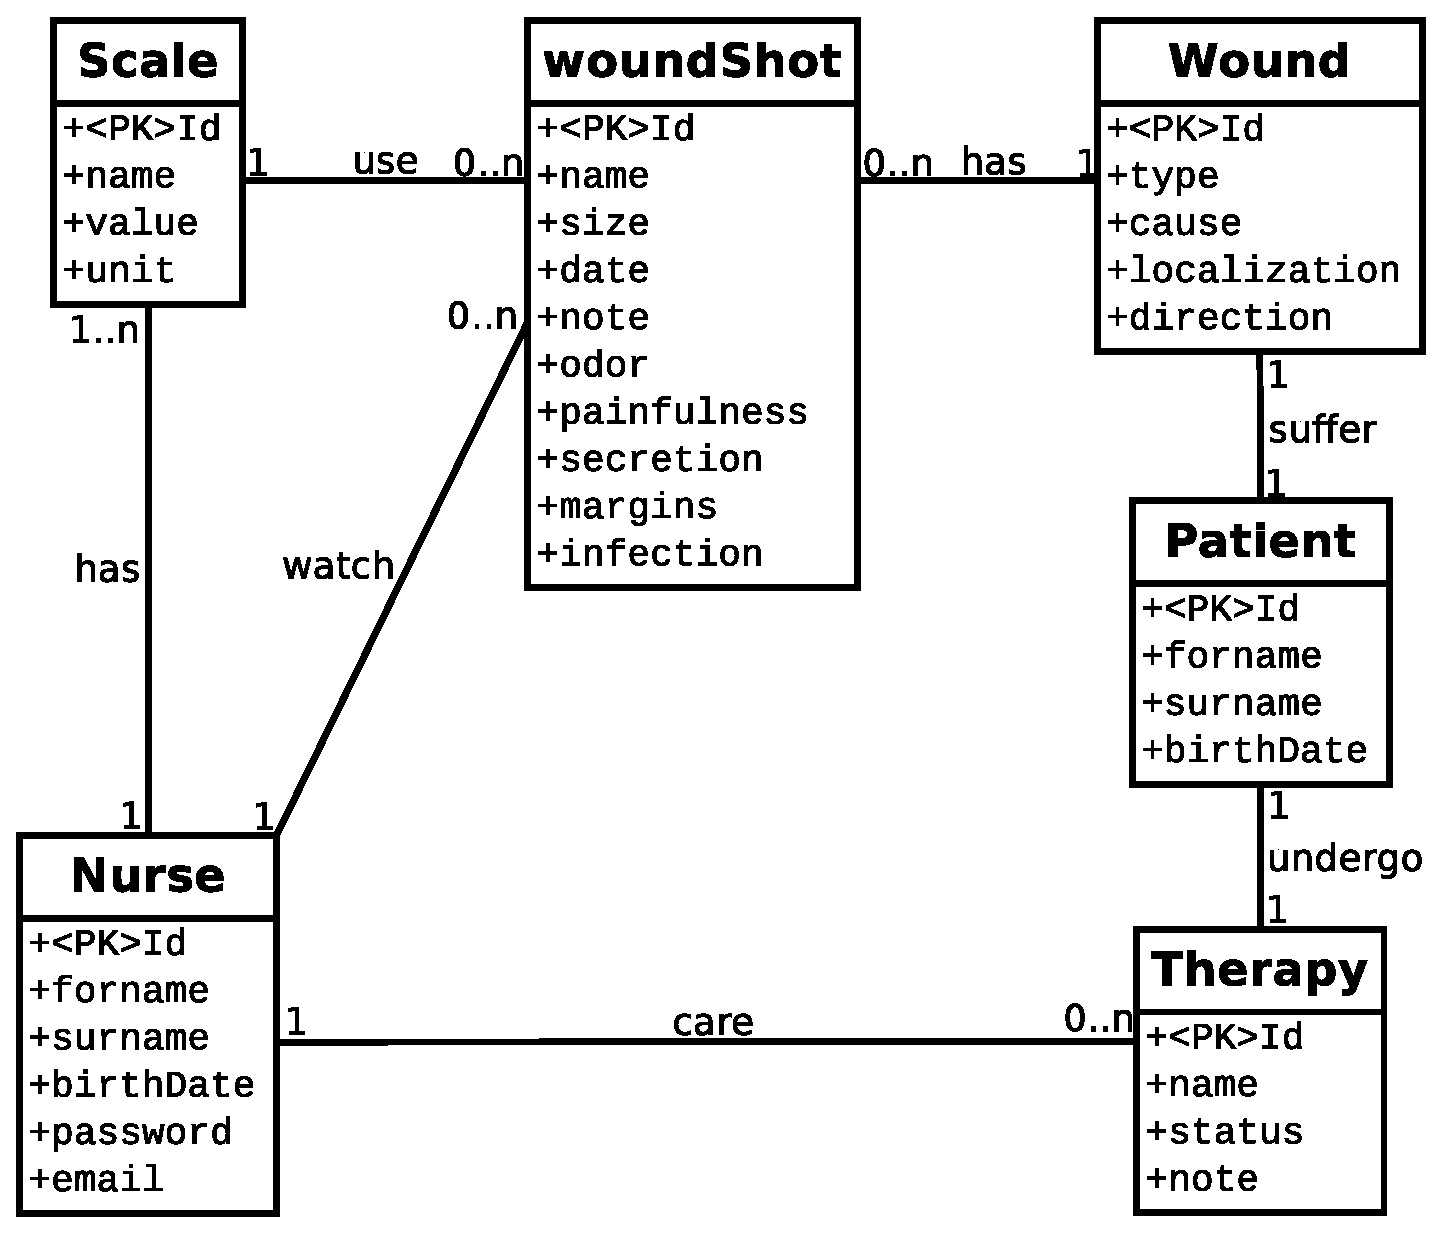
\includegraphics[scale=0.50]{fig/erd.eps}
      \caption{ER diagram návrhu databáze}
      \label{fig:erd}
\end{figure}

%%%%%%%%%%%%%%%%%%%%%%%%%%%%%%%%%%%%%%%%%%%%%%%%%%%%%%%%%%%%%%
\section{Návrh aplikačného rozhrania}
Aplikačné rozhranie by malo slúžiť ako prostredník medzi samotnou aplikáciou a databázou, ale hlavne tiež by malo slúžiť pre spracovávanie snímok chronických rán, ich detekciu, lokalizáciu a určenie plochy. Celé aplikačné rozhranie nachádzajúce sa na servery by malo byť implementované v duchu REST architektúry. Aplikácia by sa mala dotazovať na server a získavať z neho odpovede. Rozhranie by malo obsahovať 4 základné HTTP metódy ako je GET, POST, PUT a DELETE. Metóda GET by slúžila pre prístup k dátam na uložených na servery, napríklad pre získanie zoznamu liečení, alebo konkrétneho liečenia určeného svojim identifikátorom. Metóda POST by mala slúžiť pre vkladanie dát na server, napríklad pre vytváranie nového liečenia. Metóda PUT by mala slúžiť pre modifikáciu dát na servery, napríklad pre editáciu informácií o liečení. A posledná metóda DELETE by mala slúžiť pre vymazávanie dát zo serveru, napríklad odstránenie liečenia. Príklady všetkých metód na konkrétnom príklade liečení spolu s navrhnutými url adresami, na ktoré by sa malo dať dotazovať je možné vidieť v tabuľke \ref{tab:rest-example}, pričom so všetkými ostatnými dátami by sa malo pracovať rovnako (napríklad pacienti, snímky...).
\begin{table}[h]
\centering
\begin{tabular}{|l|l|l|l|}
\hline
Akcia                      & Metóda & Obsah Body                         & URL         \\ \hline
Získať zoznam liečení      & GET    & NULL                               & /therapy    \\ \hline
Získať liečenie s ID 34    & GET    & NULL                               & /therapy/34 \\ \hline
Vytvoriť nové liečenie     & POST   & \{name: "Name", status: "Active"\} & /therapy    \\ \hline
Editovať liečenie s ID 34  & PUT    & \{name: ''New Name"\}              & /therapy/34  \\ \hline
Odstrániť liečenie s ID 34 & DELETE & NULL                               & /therapy/34  \\ \hline
\end{tabular}
\caption{Príklady pre manipuláciu s liečením prostredníctvom aplikačného rozhrania.}
\label{tab:rest-example}
\end{table}

Každý dotaz by mal byť úplne definovaný a mal by obsahovať všetky potrebné informácie k jeho úspešnému vykonaniu. V prípade neúspechu by malo rozhranie vrátiť tomu odpovedajúci špecifický chybový kód. Hlavné a najbežnejšie rozšírené HTTP status kódy je možné vidieť v tabuľke \ref{tab:rest-codes}.
\begin{table}[h]
\centering
\begin{tabular}{|l|l|}
\hline
Kód                       & Význam                                                                 \\ \hline
200 OK                    & úspešná operácia a v odpovedi sa nachádzajú dáta  \\ \hline
201 Created               & operácia vkladania dát skončila úspechom                               \\ \hline
204 No Content            & úspešná operácia, ale žiadne dáta sa nenachádzajú v odpovedi \\ \hline
400 Bad Request           & server nerozumie požiadavku, kvôli nesprávnej syntaxi                  \\ \hline
401 Unauthorized          & server pre prístup k dátam vyžaduje autorizáciu                        \\ \hline
403 Forbidden             & server odmietol vykonať požiadavku                                     \\ \hline
404 Not Found             & na servery sa nenašli požadované dáta                                  \\ \hline
500 Internal Server Error & server zaznamenal neočakávanú udalosť                                  \\ \hline
\end{tabular}
\caption{Najbežnejšie používané status kódy HTTP v REST.}
\label{tab:rest-codes}
\end{table}

\chapter{Použíté technológie}
\label{chap:pouzite-techologie}
Ako už názov tejto kapitoly napovedá, kapitola predstavuje a popisuje technológie, ktoré boli vybrané v rámci návrhu a následne použité pri samotnej programovej implementácii práce. Celá implementácia, ako aj samotná kapitola, je rozdelená do logických celkov. Podľa týchto celkov bolo potrebné vybrať vhodný programovací jazyk, poprípade aplikačný rámec, pre serverovú časť (aplikačné rozhranie), klientskú časť (aplikácia) a zároveň samotnú databázu.

%%%%%%%%%%%%%%%%%%%%%%%%%%%%%%%%%%%%%%%%%%%%%%%%%%%%%%%%%%%%%%
\section{Klientská časť - aplikácia}
Klientskou časťou je v prípade tejto práce označená samotná hybridná mobilná aplikácia, poprípade aplikácia spustiteľná na desktopovom zariadení. Hybridný prístup k tvorbe aplikácie bol zvolený namiesto klasického natívneho prístupu z dôvodu, že takto vytvorené aplikácie sú vysoko multiplatformné v zmysle, že ich stačí naprogramovať raz a už iba s minimálnym zásahom do kódu pobežia takmer na väčšine bežných operačných systémov. Bol zvolený hybridný aplikačný rámec Ionic verzia 2, ktorý je postavený na programovacom jazyku Typescript (nadmnožina jazyka Javascript) a na aplikačnom rámci Angular2. Typescript sa v rámci Ionic používa na logiku aplikácie. Pre vizuál aplikácie sa používa klasické HTML a CSS, alebo preprocesor SCSS. Táto práca je zameraná na  platformu Android a platformu Windows. Platformu android je možné pokryť pomocou technológie Apache Cordova, Windows zase pomocou technológie Electron. 
\begin{itemize}
    \item \textbf{HTML -} Hyper Text Markup Language je momentálne najpoužívanejší značkovací jazyk pre tvorbu webových stránok. HTML pre popis dokumentu používa značkovacie tagy, ktoré hovoria danému programu, internetovému prehliadaču, ako má daný dokument štruktúrovať. Originálne bol tento jazyk vyvinutý pre popis štruktúry dokumentov, hlavne nadpisov, paragrafov, zoznamov, ktoré sa zdieľali medzi inštitúciami a vedeckými pracovníkmi. Postupom času sa avšak z HTML stal celosvetovo rozšírený štandard pre popis štruktúry webových stránok. V minulosti sa HTML používalo nielen pre popis štruktúry, ale aj pre popis jeho výzoru. V súčastnosti sa výzor webových stránok definuje pomocou CSS. \cite{fswG1WVQQnoCa64c}
    \item \textbf{CSS -} Cascading Style Sheet je jednoduchý dizajnérsky jazyk, ktorý popisuje ako budú dané HTML tagy zobrazené na obrazovke počítača, papieri, alebo inom médiu. Medzi hlavné výhody CSS patrí to, že šetrí čas, pretože štýl napísaný v CSS je možné potom ďalej používať na iné webové stránky a zároveň sa zrýchľuje načítanie stránok, keďže sa štýl nedefinuje väčšinou po jednom tagu, alebo po celej triede tagov. V priebehu rokov sa z CSS, tak ako to bolo aj s HTML, stal štandard pre webové stránky a podporujú ho všetky moderné webové prehliadače. \cite{VNZJ2nmvOm16rWtR}
    \item \textbf{SCSS -} Syntactically Awesome Stylesheet, je CSS preprocesor, ktorý rozširuje bežné CSS o celú radu vylepšení. Za zmienku stoja napríklad premenné, zanorovanie pravidiel, importy. To má za následok, že kód je oveľa viac organizovaný, prehľadnejší, rozsahovo menší a je možné dosiahnuť netriviálnych cieľov oveľa jednoduchšie. Jedná sa v podstate o nadmonžinu CSS. Varianta syntakticky viac podobná klasickému CSS sa nazýva SCSS (Sassy CSS). \cite{SIWRi1jHe5vClhda}
    \item \textbf{Javascript -} je interpretovaný objektovo-orientovaný programovací jazyk, ktorý je známi predovšetkým ako skriptovací jazyk používaný na webových stránkach. V kontexte webových stránok sa používa predovšetkým pre dynamickú manipuláciu, ako napríklad odozvy na rôzne udalosti, animácie a iné. Je spúšťaný webovým prehliadačom. V súčastnosti sa rozširuje aj mimo klientskú stranu webu a je ho možné vidieť ako serverové riešenie v podobe stále viac populárneho Node.js. Je založený na vytváraní prototypov. Podporuje imperatívne, ale aj funkcionálne programovanie. \cite{mpahm68E0P8GyL7C}
    \item \textbf{Typescript -} Ako aplikácia napísaná v Javascripte rastie, tak začína byť neprehľadná a ťažko udržovateľná. Z toho dôvodu Microsoft vyvinul Typescript. Typescript je vlastne nadmnožina Javascriptu, ktorá nezahŕňa iba samotný jazyk, ale aj početnú sadu nástrojov. Všetok kód napísaný v Typescripte sa transpiluje do čistého Javascriptu. Typescript rozširuje obyčajný Javascript o silné statické typovanie a je plne objektovo orientovaný (je možné použiť dedičnosť, triedy, rozhrania a iné veci typické pre čisto objektovo orientované jazyky). V neposlednom rade je v ňom možné používať všetky bežné Javascriptové knižnice. \cite{f7jKojjQlPsziQuS}
    \item \textbf{Angular2 -} je Typescriptový aplikačný rámec pre tvorbu webových tzv. Single Page aplikácií. Je vyvinutý týmom z Googlu, ktorý pracoval aj na originálnom AngularJS. Aj keď Angular2 a AngularJS majú podobné princípy, prakticky ide o dva odlišné aplikačné rámce. Tento rámec bol prvý krát predstavený v roku 2014. Jeho myšlienka je založená na tvorbe znovupoužiteľných komponentov a v podstate využíva o Model Controler View architektúru, ktorú je ale možné vymeniť napríklad za architektúru Redux, známu hlavne z Facebook rámca React. \cite{oHlcq3e3366Aa2oa}
    
    Single page aplikácie sú webové aplikácie, ktoré používajú väčšinou server iba ako zdroj a úložisko dát. Získané dáta sú následne vykresľované na klientovi pomocou Javascriptu. Pri prvom príchode na takúto stránku sa najprv stiahnu potrebné Javascriptové súbory a základná kostra HTML. Následne sa vykonajú operácie, ktoré určia, čo sa má zobraziť. Podľa toho čo sa má zobraziť je asynchrónnym dotazom (AJAX) na server požiadané o dáta, ktoré prídu v odpovedi typicky vo formáte JSON. Pri ďalšej interakcií so stránkou sa robia vždy len dotazy na samotný obsah. Server je v prípade takýchto webových stránok pasovaný iba do jednoduchého rozhrania, ktoré spracováva požiadavky z klienta a poprípade získava a ukladá dáta. \cite{Jahoda2015}
    \begin{figure}[h]
        \centering
        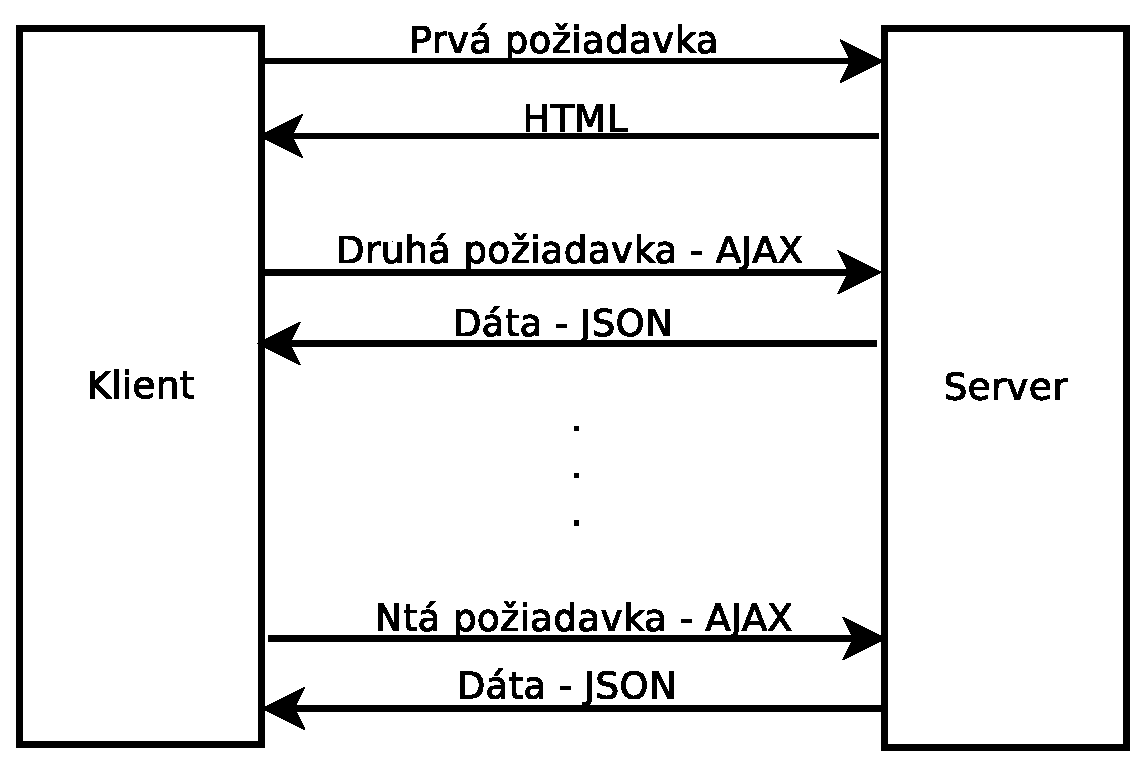
\includegraphics[scale=0.5]{fig/spa.eps}
        \caption{Klient-server komunikácia v Single page aplikácii.}
        \label{fig:spa}
    \end{figure}
    \pagebreak
    \item \textbf{Cordova -} je rámec, ktorý zabalí HTML, CSS a Javascript aplikáciu do natívneho kontaineru, WebView, ktorý vo výsledku vyzerá a chová sa ako bežná natívna aplikácia. Kontainer dokáže pristupovať k funkciám zariadenia vďaka natívnym zásuvným modulom a Javascriptovému aplikačnému rozhraniu. Cordova podporuje celú škálu platforiem od Android, cez iOS, až po Windows Phone. Projekt bol najprv vytvorený firmou Nitobi, ktorá bola v roku 2011 kúpená známou firmou Adobe Systems. Adobe Systems následne uvoľnila kód Cordovy. \cite{DVKuXjtaapUpB12M}
    \begin{figure}[h]
      \centering
      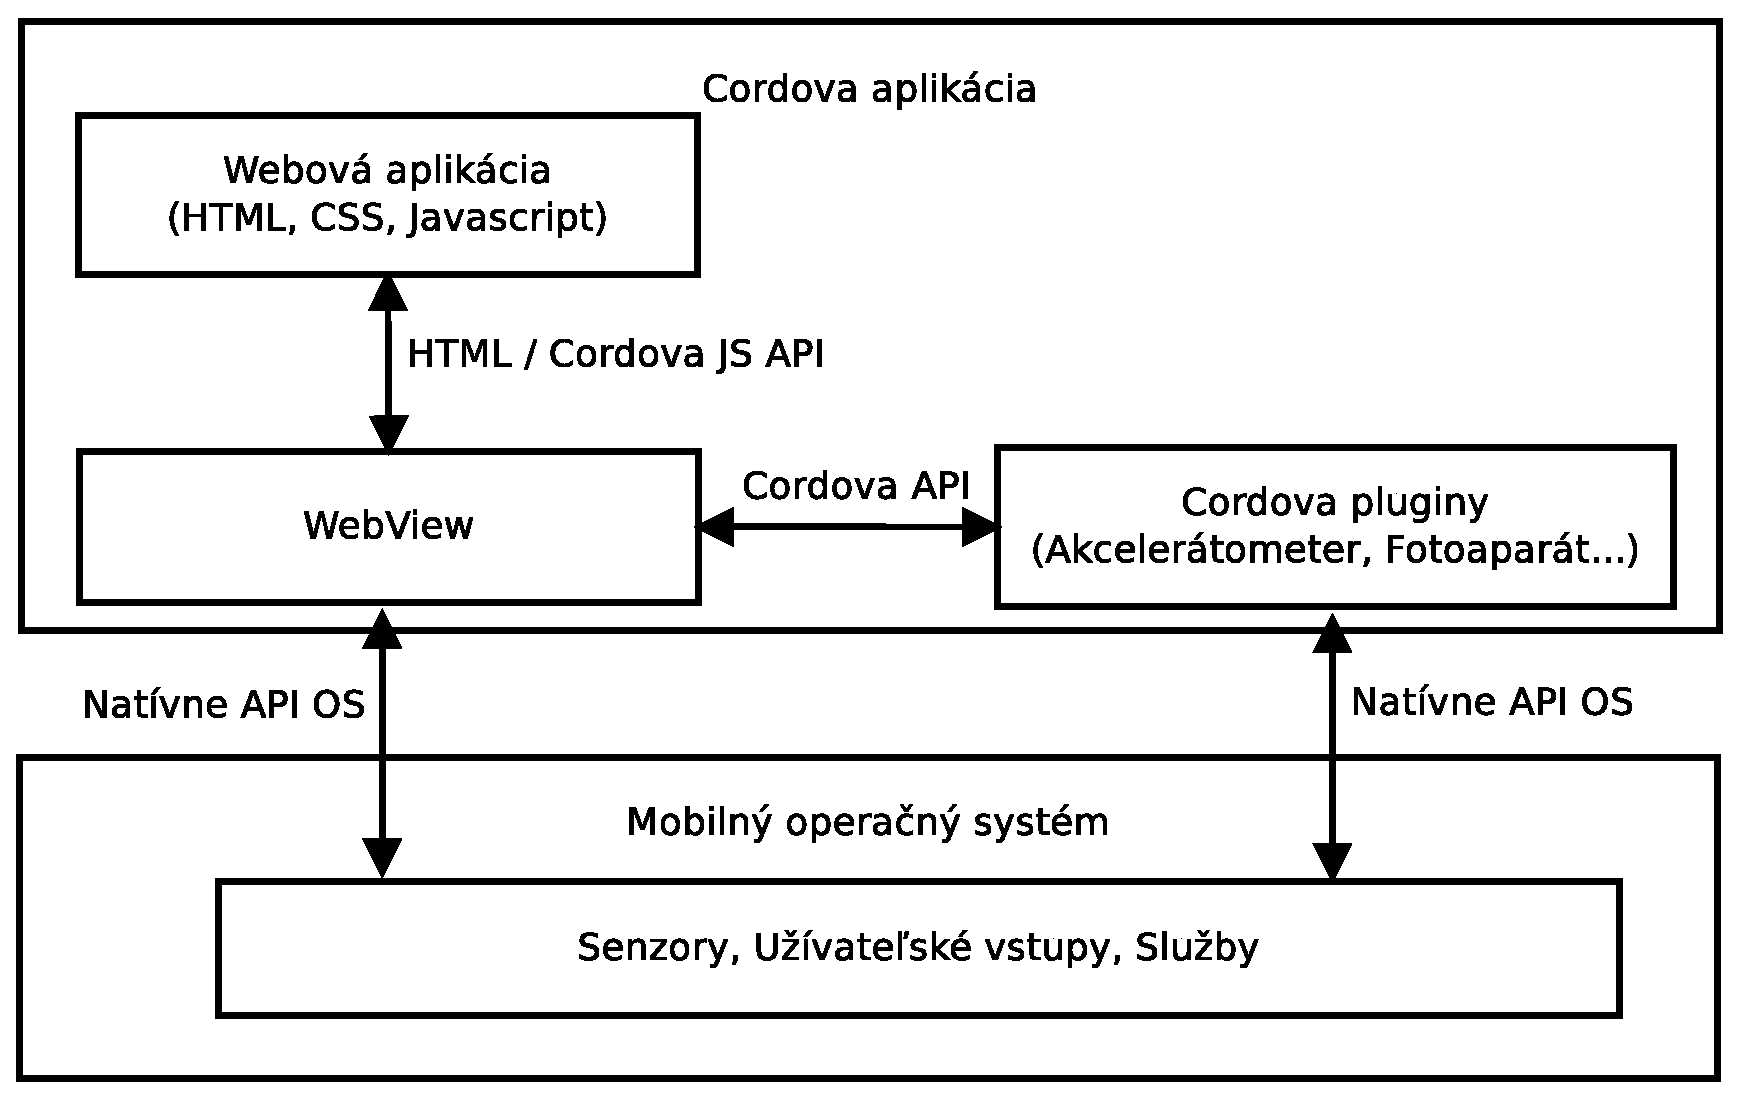
\includegraphics[scale=0.35]{fig/cordova.eps}
      \caption{Architektúra aplikácie vytvorenej pomocou Cordova technológie.}
      \label{fig:cordova}
    \end{figure}
    \item \textbf{Ionic2 -} je kompletné SDK pre vývoj hybridných mobilných aplikácií. Celý aplikačný rámec je postavený na Angular2 a  rozširuje ho o ďalšie komponenty a funkcionalitu typickú pre mobilné zariadenia. Pomocou Cordova zásuvným modulom a ich implementácií v tomto rámci je možné tiež pristupovať k natívnym funkciám zariadenia. \cite{HiUt1XS9KvN1fiB5}
    
    Hybridné mobilné aplikácie sú aplikácie, ktoré na prvý pohľad vypadajú ako natívne aplikácie, avšak ich programovanie prebiehalo väčšinou pomocou webových technológií s následným zabalením pomocou technológie Cordova, alebo inej podobnej. Medzi  najväčšiu výhodu takéhoto prístupu patrí to, že aplikáciu stačí napísať iba raz a potom ju je možné už iba s drobnými zmenami vydávať na rôzne mobilné platformy.\cite{0QSW9GoG0OTJ7FKM}
    \item \textbf{Electron -} je knižnica vyvinutá GitHubom pre tvorbu multiplatformných desktopových aplikácií pomocou webových technológií, ktoré už boli popísané. Electron je ponúkaný pod licenciou MIT a má otvorený kód. Využíva kombináciu technológie Chromium a Node.js, ktoré zabalí spolu s webovou aplikáciou do jednej výslednej aplikácie. Takúto výslednú aplikáciu je možné spúšťať na platforme Windows, Mac a aj Linux. K natívnym funkciám operačného systému je možné pristupovať, tak ako v prípade Cordovy, pomoocu natívnych aplikačných rozhraní. \cite{hBGbGXxiU66nJt51}
    \begin{figure}[h]
      \centering
      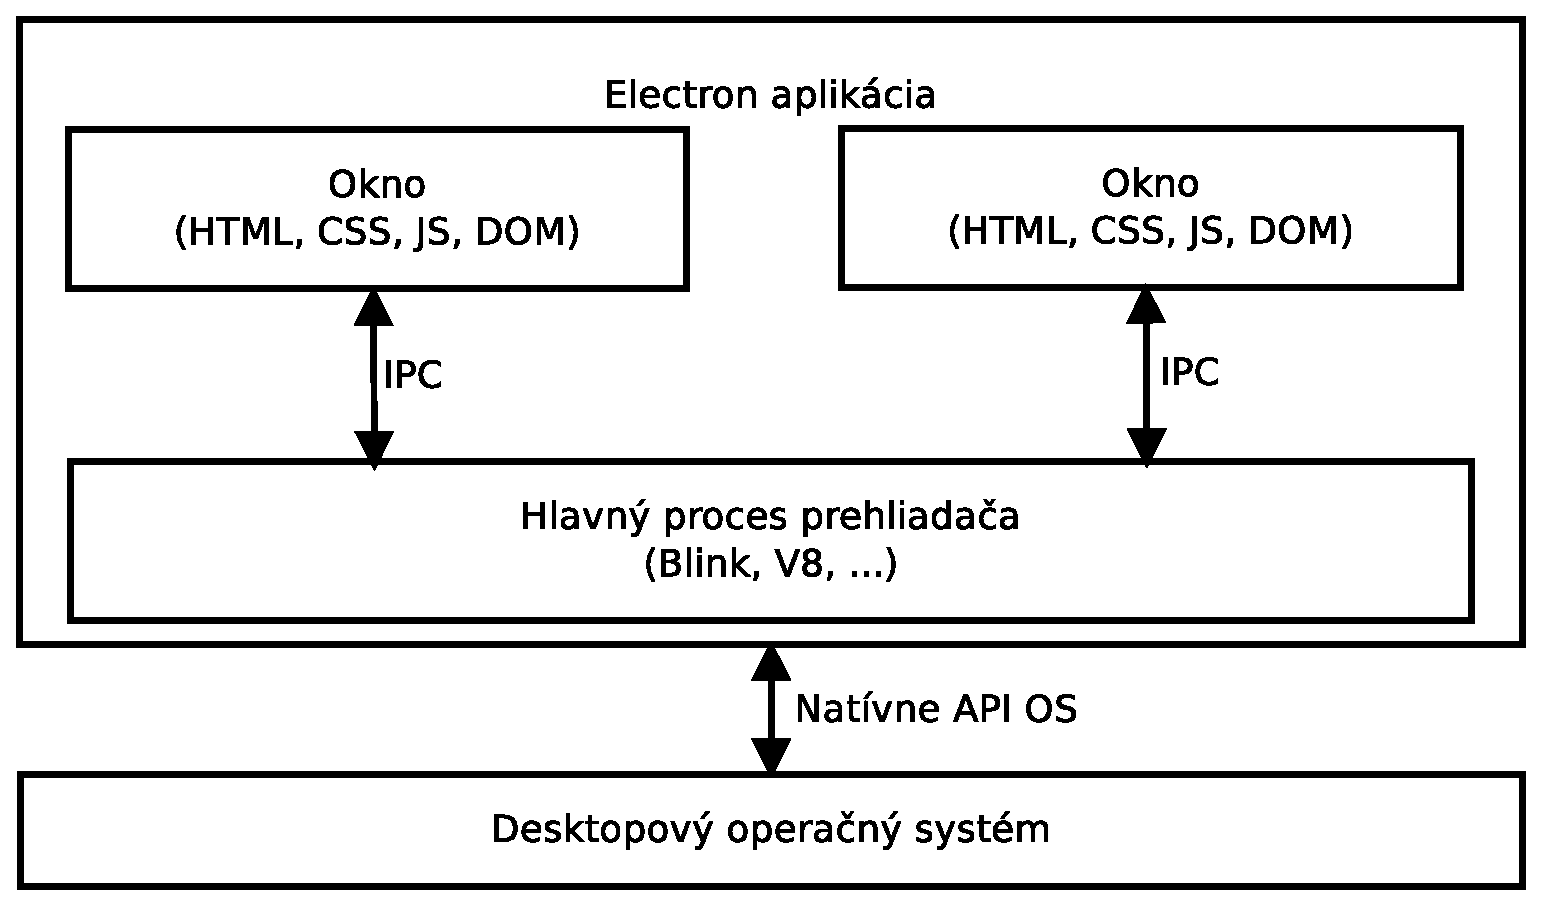
\includegraphics[scale=0.40]{fig/electron.eps}
      \caption{Architektúra aplikácie vytvorenej pomocou Electron rámca.}
      \label{fig:electron}
    \end{figure}
\end{itemize}

%%%%%%%%%%%%%%%%%%%%%%%%%%%%%%%%%%%%%%%%%%%%%%%%%%%%%%%%%%%%%%
\section{Databázová časť}
Pre uchovanie dát na strane serveru bola zvolená možnosť uloženia do databáze. Táto možnosť bola zvolená kvôli tomu, že manipulácia s dátami je pomerne rýchla, keďže sa do pamäte neukladá celá databáza, ale iba jej požadovaná časť. Okrem toho, pre získanie dát sa dá použiť pokročilejší dotazovací jazyk a je podporovaný prístup viacerých užívateľov súčasne. 

Ako databáza bol zvolený typický zástupca NoSQL databáz menom MongoDB, ktorý je vyvíjaný MongoDB industries a má otvorený zdrojový kód. Dáta ukladá v štruktúre podobnej JSON dokumentom, a to v štruktúre Binary JSON, ktorý samotný JSON obohacuje o ďalšie typy. Súvisiace informácie sú uložené spolu pre rýchly dotazovací prístup pomocou MongoDB dotazovacieho jazyka. Používa dynamické schémy, to znamená, že záznamy nemajú pevne danú štruktúru a v priebehu sa táto štruktúra môže meniť. Pomocou tohoto dátového modelu je možné reprezentovať hierarchické vzťahy a ukladať polia a iné komplexnejšie dátové štruktúry. MongoDB dbá na to, aby bola zabezpečená vysoká dostupnosť a škálovateľnosť. Nespornou výhodou NoSQL a konkrétne MongoDB oproti Mysql je, že vývoj aplikácie s MongoDB je jednoduchší, keďže sa dokumenty v databáze prirodzene mapujú do moderných objektovo orientovaných jazykov a odpadá tak objektovo relačné mapovanie objektov. Obrovskou výhodou oproti napríklad MySQL je už spomínaná škálovateľnosť. Samotné MongoDB vyžaduje pre svoje fungovanie iba adresár na uloženie dát a teda môže byť ľahko distribuované spolu s programom. \cite{Banker2011}
\begin{lstlisting}[caption={Ukážka štruktúry NoSQL MongoDB databáze.},captionpos=b]
[
    item1ID: {
	    name: 'MongoDB',
	    description: 'NoSQL'
    },
    item2ID: {
	    name: 'MySQL',
	    description: 'Relational'
    }
]
\end{lstlisting}

%%%%%%%%%%%%%%%%%%%%%%%%%%%%%%%%%%%%%%%%%%%%%%%%%%%%%%%%%%%%%%
\section{Serverová časť - aplikačné rozhranie}
Serverová časť pokrýva všetky operácie, ktoré sa nevykonávajú priamo v zariadení, ale vykonávajú sa vzdialene na strane serveru. Medzi takéto operácie patrí napríklad ukladanie dát do databáze, autentifikácia, autorizácia užívateľa, alebo samotná práca so snímkom chronickej rany. Serverová časť v tejto práci tvorí vzdialené aplikačné rozhranie. Je tvorená pomocou skriptovacieho jazyka Python, za pomoci aplikačného rámca Flask. Flask vo svojom jadre dodržiava princípy REST a je vďaka tomu možné jednoducho navrhnúť plne funkčné RESTful aplikačné rozhranie, s ktorým v tejto práci priamo komunikuje klientská aplikácia. Pre spracovanie obrazu, konkrétne samotných fotiek chronických rán, bola vybraná Python implementácia populárnej knižnice na spracovanie obrazu zvaná OpenCV.
\begin{itemize}
    \item \textbf{REST -} Representational state transfer je súbor niekoľkých prísnych, ale jasne definovaných pravidiel pre návrh architektúry distribuovaného systému, hlavne rozhrania medzi jednotlivými komponentami, poprípade serverovou a klientskou časťou. Základným stavebným kameňom RESTu je zdroj. Zdroj môže byť čokoľvek, napríklad konkrétny objekt v databáze, dokument a podobne. Základným pravidlom je, že každý objekt musí mať svoju URL. Klient nikdy nevidí zdroj priamo, ale vždy iba jeden z jeho obrazov, ktorý je nazývaný reprezentácia. Reprezentácia je strojovo čitateľná reprezentácia aktuálneho stavu zdroja. Môže to byť obrázok, HTML stránka a podobne. Výber reprezentácie môže byť ovplyvnený klientom pomocou riadiacej informácie, alebo serverom na základe klasifikácie klienta. Samotná komunikácia cez REST je bezstavová, čo znamená, že každý požiadavok obsahuje všetky informácie potrebné k jeho vykonaniu. REST definuje 4 základné operácie: POST pre vytváranie, GET pre získavanie, PUT pre zmenu a DELETE pre vymazávanie. \cite{Allamarajuc2010, 54r2mhdAeuyxzZPp}
    \item \textbf{Python -} je open source objektovo-orientovaný vysokoúrovňový skriptovaci jazyk, ktorý vytvoril Guido van Rossum v rokoch 1985-1990. Kód Pythonu spadá pod licenciu GNU General Public License. Python je interpretovaný a teda nie je nutné programy v ňom napísané prekladať. Programy sú namiesto prekladu priamo vykonávané interpreterom. Okrem toho je taktiež interaktívny. To znamená, že užívateľ môže priamo interagovať s interpreterom a písať programy aj týmto spôsobom. Ďalšou nespornou výhodou Pythonu je to, že je rozšíriteľný a nízko-úrovňové moduly sa dajú písať v programovacom jazyku C. Vďaka tomu môže byť dosiahnuté lepšej efektivity. \cite{CCnsn576LIGBCH2C}
    
    Python bol zvolený najmä kvôli tomu, že je pomerne rozšírený, bežne sa používa na serverovú časť webových informačných systémov, má na výber z veľkého množstva intuitívnych aplikačných rámcov, dobre si rozumie s relačnými, ale aj s NoQSL databázami a v neposlednom rade je preň dostupná implementácia OpenCV.
    \item \textbf{Flask -} je aplikačný mini rámec, ktorý je napísaný v programovacom jazyku Python. Slúži pre vývoj webových aplikácií, alebo vo všeobecnosti serverových častí informačných systémov, poprípade aplikačných rozhraní. V základe má k dispozícií iba funkcie s prácou pre URL, HTTP a šablónami. Z toho plynie, že je jednoduchý na osvojenie a pre účely tejto práce úplne postačuje. \cite{YNlrXY2RKWca3gk8}
    \item \textbf{OpenCV -} je knižnica počítačového videnia. Je napísaná v jazyku C a C++ a je možné ju použiť na všetkých bežných aktuálnych platformách. Rozhranie je dostupné pre Python, Java, Ruby a ostatné bežné programovacie jazyky. OpenCV bolo navrhnuté pre výpočtovú efektivitu so silným dôrazom na aplikácie bežiace v reálnom čase. Optimalizácie knižnice boli vykonávané na všetkých úrovniach, od algoritmov až po viac jadrové inštrukcie procesorov. Hlavným cieľom je ponúknuť jednoduchú infraštruktúru počítačového videnia, ktorá by pomáhala ľuďom tvoriť zložitejšie aplikácie oveľa rýchlejšie a jednoduchšie. Samotná knižnica obsahuje viac ako 500 funkcií, pokrývajúce rôzne odvetvia vedy. OpenCV v sebe obsahuje okrem svojej samotnej implementácie aj pod-knižnice pre strojové učenie. keďže počítačové videnie a strojové učenie spolu úzko súvisia. Pod-knižnice sa z veľkej časti orientujú na rozpoznávanie vzorov a rozdeľovanie do zhlukov. \cite{Bradskic2008}
\end{itemize}

\chapter{Implementácia}
\label{chap:implementacia}
Táto kapitola pojednáva o samotnej programovej realizácií a približuje implementačné detaily tejto diplomovej práce. Kapitola vychádza z informácií uvedených v predchádzajúcich kapitolách, presnejšie popisuje prevod návrhov vykonaných v kapitole \ref{chap:analyza-navrh-riesenia} na konkrétne programové riešenie, pri ktorom boli použité technológie popísané v kapitole \ref{chap:pouzite-techologie}.  Rovnako, ako aj kapitola o analýze a návrhu riešenia, tak aj táto kapitola je rozdelená do niekoľkých logických celkov. Najprv je popísaná implementácia klientskej, či už mobilnej, alebo desktopovej aplikácie. V poradí druhou časťou je popis finálnej formy databáze, ktorá je ihneď nasledovaná popisom implementácie serverového aplikačného rozhrania, pod ktoré  spadá aj práca so snímkami. Celá kapitola je na záver ukončená popisom vybraných významnejších implementančných detailov ako je napríklad prihlasovanie, získavanie snímkov, alebo generovanie PDF súborov.

%%%%%%%%%%%%%%%%%%%%%%%%%%%%%%%%%%%%%%%%%%%%%%%%%%%%%%%%%%%%%%
\section{Implementácia klientskej aplikácie}
Aplikácia, ako sa píše už v kapitole \ref{chap:pouzite-techologie}, je implementovaná pomocou rámca pre vývoj hybridných mobilných aplikácií menom Ionic. Funkčnosť na mobilnom zariadení so systémom Android zabezpečuje rámec Cordova a na desktopovom zariadení so systémom Windows zase rámec Electron.

\subsection{Štruktúra aplikácie a popis jej komponentov}
Celá aplikácia je umiestnená v zložke \textit{src} a pozostáva z niekoľkých typov tried. Každý typ triedy je umiestnený vo vlastnom priečinku, ktorý je pomenovaný podľa tohoto typu. Konkrétne sa jedná o priečinok \textit{app}, \textit{effects}, \textit{enum}, \textit{model}, \textit{pages}, \textit{providers} a priečinok \textit{reducers}. Okrem týchto typov priečinok \textit{src} obsahuje ešte konfiguračné súbory spolu so zložkou \textit{assets} a \textit{theme}. Priečinok \textit{assets} obsahuje všetky statické súbory, ktoré sa netranspilujú \footnote{Transpilácia je proces prekladu zdrojového kódu daného jazyka na zdrojový kód iného jazyka, v prípade práce z Typescriptu na Javascript \cite{Sengstacke2542016}}, konkrétne sa jedná o ikonu aplikácie spolu s obrázkom tlačidla na prihlasovanie Google účtom. Priečinok \textit{theme} obsahuje súbory, poprípade iba jeden súbor, ktorý predstavuje globálnu tému aplikácie, ktorá v sebe drží definície farieb, definície štýlov písma a iné podobné nastavenia globálneho charakteru.

V zložke \textit{app} sa nachádza hlavná komponenta a modul, ktorý predstavujú celú aplikáciu. V \textit{app} module sa nachádzajú všetky definície používaných stránok, poskytovateľov služieb, reduktorov, efektov, modálnych okien a poprípade, ak by sa v tejto práci využívali, aj direktív a rúr. Každá komponenta, a nie je tomu inak ani pri \textit{app} komponente, sa skladá vždy z troch hlavných typov súborov. Z typescript súboru, z html súboru a z scss súboru. 
\begin{itemize}
\item Typescript súbor predstavuje akýsi kontrolér danej komponenty poprípade jej logiku. 
\item Html súbor predstavuje pohľad a obsahuje zobrazované dáta jednosmerne, alebo obojsmerne naviazané na dáta v typescript súbore. 
\item Scss súbor definuje vzhľad zobrazovaného html dokumentu, avšak aplikácia v tejto práce si vystačí s bežnými komponentami Ionic rámca a tento súbor je preto často prázdny.
\end{itemize}
\textit{App} komponenta je špeciálna tým, že je globálna a existuje po celú dobu aplikácie a
preto obsahuje hlavné menu a udalosti a funkcie viazané hlavne k tomuto hlavnému menu. Vďaka tomuto menu je možné prechádzať medzi stránkami aplikácie, alebo sa odhlasovať.

V priečinku \textit{models} sa nachádzajú modely, alebo konkrétne rozhrania, všetkých hlavných entít použitých v tejto práci, menovite to sú \textit{scale.model}, \textit{therapy.model}, \textit{user.model} a \textit{wound.model}. Tieto rozhrania zabezpečujú typovú kontrolu daných entít a okrem toho behom vývoja aplikácie zabezpečovali inteligentné našeptávanie. Mimo samotných modelov, sa v tomto priečinku nachádza ešte súbor \textit{app.state}, ktorý predstavuje hlavný stav aplikácie a taktiež môže byť chápaný, ako akýsi model. \textit{App.state} slúži pre prácu s \textit{ngrx storom}, jeho efektmi a reduktormi. Celý stav aplikácie je vďaka nemu rozdelený na niekoľko podstavov určitého typu podľa vlastností tohoto \textit{app.state modelu}. Ide napríklad o typ \textit{therapy}, \textit{wound}, alebo iný a je vďaka tomu umožnené pracovať iba s vybranou časťou celkového stavu aplikácie.

V priečinku \textit{enums} sa zase nachádzajú všetky vymenúvacie typy, poprípade konštanty, ktoré sa v rámci aplikácie nemenia a sú tu definované nemenne, napevno. Ide napríklad o typy mierok, alebo stavy liečenia.

Priečinok \textit{reducers} obsahuje reduktory, ktoré slúžia na manipuláciu so stavom aplikácie. Stav aplikácie je vlastne nemenná dátová štruktúra. Stav aplikácie sa teda nemodifikuje, ale nahrádza sa vždy novým stavom. Na zmenu stavu, alebo presnejšie povedané jeho nahradenie, slúžia akcie, ktoré presne popisujú a definujú, ako sa daný stav zmení. Tieto zložky dohromady tvoria \textit{ngrx store}. Ngrx store je vlastne kontajner, alebo menežment stavu aplikácie založený na RxJS určený pre Angular a je inšpirovaný stále viac populárnym Redux. Hlavnou myšlienkou je umožnenie vytvárania komponentov schopných používať stratégiu detekcie zmeny nazvanú \textit{OnPush}.\cite{nic5zZJbUwJyjA3R} Komponenty teda načúvajú zmene stavu aplikácie, alebo jeho časti a následne na to reagujú. Všetky súbory reduktorov v sebe obsahujú okrem funkcie na zmenu stavu aj definíciu spomínaných akcií. Stav tejto aplikácie sa skladá, ako už bolo niekoľko krát spomenuté, z niekoľkých častí. Konkrétne sa jedná o časť zoznamu mierok, zoznamu liečení, zoznamu rán a o časť jednotlivej terapie a jednotlivej rany. Veľkou výhodou takéhoto prístupu je, že stačí odoslať konkrétnu akciu na \textit{ngrx store} a zmenené dáta automaticky dostanú všetky komponenty, ktoré čakajú na zmenu danej časti stavu. Tento prístup sa ukázal ako veľmi vyhovujúci, nakoľko aj pri nie až tak rozsiahlej aplikácií, ako je aplikácia tejto práce, vznikalo početné množstvo závislostí, kedy zmena dát na nejakom mieste  vyžadovala ešte aj zmenu dát na niekoľkých iných miestach.

Efekty, ktoré sú umiestnené v rovnomennej zložke \textit{effects} sú taktiež súčasťou \textit{ngrx store}. Jedná sa vlastne o akési vedľajšie účinky odoslania akcie, kedy sa nemení stav aplikácie, ale pred zmenou stavu aplikácie sa odošle ešte napríklad požiadavka na aplikačný server a získajú sa dáta. Dokončenie tejto akcie vyvolá zmenu stavu, veľmi často zmenu stavu pomocou už získaných dát zo serveru.\cite{pzU1UYWXatJMcZgL} Obrázok \ref{fig:ngrx} popisuje konkrétny prípad chovania v aplikácií, kedy sa vyvolá akcia \textit{GET\_REQUEST}. Túto akciu zachytí ako reduktor, tak aj efekt. Reduktor na akciu zareaguje tak, že iba vráti rovnakú kópiu stavu. Avšak efekt na akciu zareaguje tak, že sa vykoná požiadavka na aplikačný server a podľa úspechu/neúspechu operácie sa vyvolá akcia \textit{GET\_SUCCESS}/\textit{GET\_REQUEST} s dátami a tento nový stav je potom uložený do \textit{ngrx store}. \textit{Ngrx store} nakoniec tento stav vráti nejakej načúvajúcej komponente/komponentám. 
\begin{figure}[h]
  \centering
  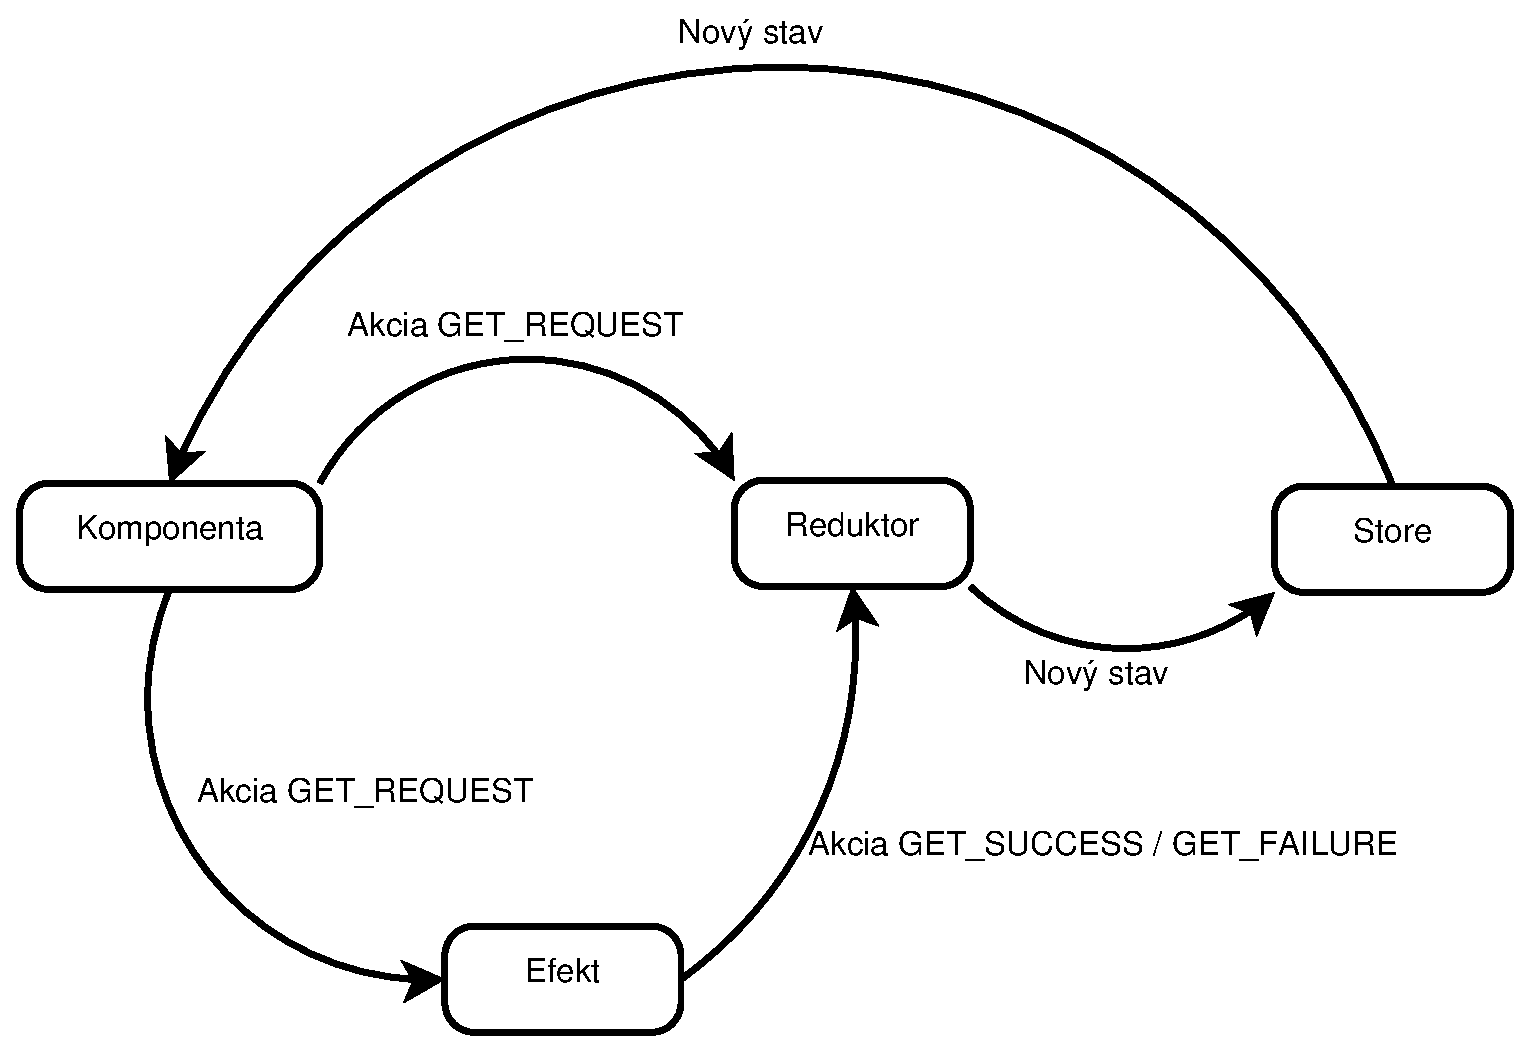
\includegraphics[scale=0.4]{fig/ngrx-efekt.eps}
  \caption{Tok dát aplikácie využívajúcej ngrx store}
  \label{fig:ngrx}
\end{figure}

Poskytovatelia nachádzajúci sa v priečinku \textit{providers slúžia}, ako názov napovedá na poskytovanie dát, či už nemenne uvedených v triede, alebo získaných z aplikačného serveru. Okrem získavania dát môžu obsahovať funkcie používané v rôznych častiach aplikácie a tak odprosťovať od písania opakovaných úsekov kódu. Jedná sa spravidla o triedy návrhového vzoru singleton\footnote{Singleton je návrhový vzor, ktorého podstatou je vytvorenie iba jednej inštancie triedy, ktorá sa používa naprieč celou aplikáciou.\cite{lREQ9U50PweZWx0G}}, teda vzoru, ktorý sa v rámci aplikácie nachádza iba raz a inštancie týchto tried sú držané v \textit{dependency injection}\footnote{Dependency injection je návrhový vzor, v ktorom trieda dostáva svoje závislosti z externých zdrojov namiesto toho, aby si ich vytvárala sama.\cite{huX3wRi17CwZ4WPd}} kontajnere aby k nim mohli pristupovať komponenty a tak využívať ich funkcionalitu a dáta. V tejto aplikácií sa využíva celkom 5 poskytovateľov. 
\begin{itemize}
\item Api poskytovateľ (\textit{api.provider}) slúži na komunikáciu medzi aplikáciou a aplikačným serverom. Obsahuje metódy na vytváranie, mazanie a získavanie zdrojov serveru podľa daných parametrov. 
\item Auth poskytovateľ (\textit{auth.provider}) slúži na autentifikáciu a operácie k tomu príbuzné. Konkrétne obsahuje metódy na prihlasovanie, zaregistrovanie, odhlasovanie, zistenie stavu prihlásenia a taktiež drží informácie o aktuálne prihlásenom užívateľovi. 
\item Poskytovateľ dočasných náhradných dát (\textit{mock-data.provider}) slúžil počas vývoja na poskytovanie predpripravených dát pre rýchlejší vývoj, kedy sa pracovalo s týmito konštantnými dátami namiesto reálnych dát. 
\item Poskytovateľ elementov užívateľského prostredia (\textit{ui-elements.provider}) zapúzdruje niektoré často používané funkcie samotného Ionic rámca. Ide napríklad o vytváranie a zobrazovanie grafických užívateľských elementov nazvaných \textit{Toast}, alebo \textit{Alert}. Funkcie tohoto poskytovateľa takto obsahujú funkcie rámca a presnejšie špecifikujú chovanie týchto funkcií pomocou parametrov. 
\item Poskytovateľ všeobecných funkcií je posledným poskytovateľom. Tento poskytovateľ obsahuje funkcie, ktoré neboli zaradené do žiadneho iného poskytovateľa. Konkrétne tento poskytovateľ obsahuje iba 2 funkcie, a to funkciu na odstránenie vlastnosti \textit{id} a mapovanie \textit{\_id->\$oid} na \textit{id}. Funkcie sú prítomné preto, že na strane serveru a na klientskej strane sa pracuje s identifikátormi odlišne. Je to paradoxne pre jednoduchšiu prácu na klientovi, pretože databáza pracuje so svojou špecifickou štruktúrou identifikátorov a tá na klientskej strane nebola potrebná.
\end{itemize}

Posledným a zároveň aj najdôležitejším, najbohatším priečinkom na informácie a funkcionalitu je priečinok \textit{pages}. Tento priečinok obsahuje všetky stránky, obrazovky aplikácie. V koreni adresára sa nachádzajú vždy priečinky hlavných stránok. V týchto priečinkoch sa nachádzajú potom okrem samotných zdrojových súborov stránok ešte aj ďalšie stránky, alebo komponenty, ktoré súvisia s danou nadradenou stránkou sa sú v nej v podstate vnorené. Takýmto príkladom môže byť modálne okno, ktoré síce vyzerá ako stránka, ale je to vo svojej podstate súčasť inej stránky. Každá stránka, ako už bolo spomenuté pri \textit{app} module, sa skladá z niekoľkých súborov. Z typescript súboru plniaceho funkciu kontroléru. Z scss súboru, ktorý definuje výzor danej stránky a je v aplikácií v podstate skoro nepoužívaný, keďže sa používajú zväčša neupravené Ionic komponenty už v úhľadnej Material design forme. Z html súboru, ktorý predstavuje pohľad na dáta z kontroléru a definuje štruktúru stránky. A nakoniec z modulu, ktorý je prítomný iba aby bolo možné prepojiť stránky s hlavným \textit{app} modulom. Samotná aplikácia obsahuje 6 hlavných stránok. Ide o stránku obsahujúcu informácie o aplikácií (\textit{About}), stránku slúžiacu na prihlásenie (\textit{Login}), stránku obsahujúcu nastavenie a vytváranie mierok (\textit{Settings}), stránku obsahujúcu zoznam liečení (\textit{Therapy list}), stránku zobrazujúcu detail liečenia (\textit{Therapy detail}) a nakoniec stránku obsahujúcu detail rany, samotnú konkrétne zachytenú snímku (\textit{Wounbd detail}). Štruktúru členenia stránok je možné vidieť na obrázku \ref{fig:pages}.
\begin{figure}[h]
  \centering
  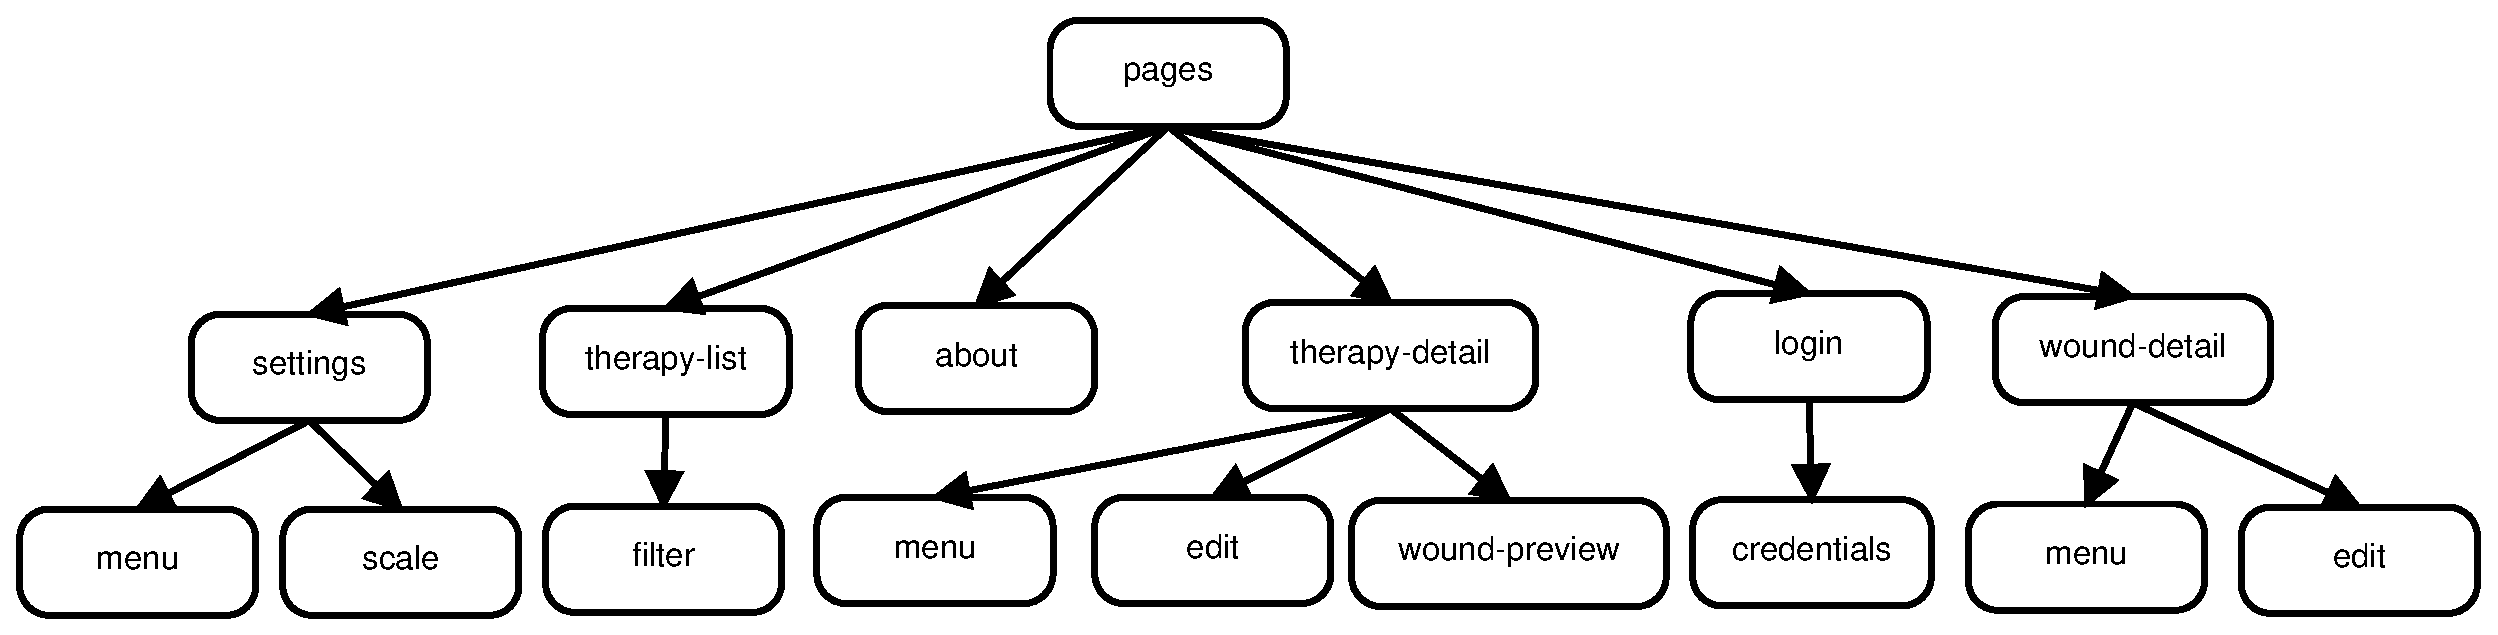
\includegraphics[scale=0.364]{fig/pages.eps}
  \caption{Štruktúra členenia stránok a ich komponentov}
  \label{fig:pages}
\end{figure}

Z obrázka je teda jasne vidieť, aké komponenty a stránky obsahujú hlavné stránky. Je zreteľne vidieť, že väčšina stránok obsahuje komponentu \textit{menu}, poprípade \textit{filter}, ako to je pri stránke zoznamu liečení, čo je vlastne kontextové menu umiestnené v pravom hornom rohu hlavičky aplikácie. Okrem komponenty \textit{menu} väčšina stránok tiež obsahuje podstránku \textit{edit}. Táto podstránka je vlastne modálne okno slúžiace na vytváranie, poprípade editovanie daného vybraného zdroja. Implementované stránky je možné vidieť na obrázkoch \ref{fig:app1} až \ref{fig:app4}.
 \begin{figure}[h]
   \begin{minipage}{0.48\textwidth}
     \centering
     
\includegraphics[scale=0.60]{fig/app1.png}
      \caption{Obrazovka zoznamu liečení}
      \label{fig:app1}
   \end{minipage}\hfill
   \begin{minipage}{0.48\textwidth}
     \centering
     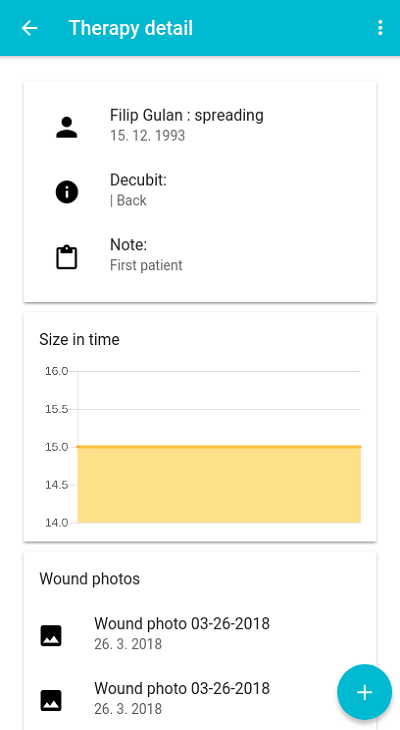
\includegraphics[scale=0.60]{fig/app2.png}
      \caption{Obrazovka detailu liečenia}
      \label{fig:app2}
   \end{minipage}
\end{figure}
\begin{figure}[h]
   \begin{minipage}{0.48\textwidth}
     \centering
     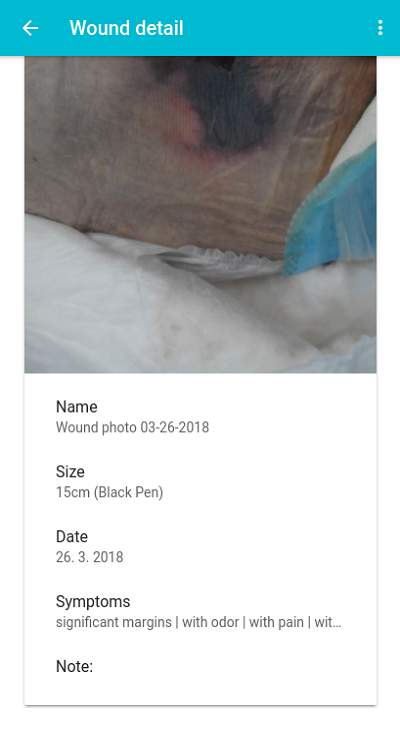
\includegraphics[scale=0.60]{fig/app3.png}
      \caption{Obrazovka detailu rany}
      \label{fig:app3}
   \end{minipage}\hfill
   \begin{minipage}{0.48\textwidth}
     \centering
     
\includegraphics[scale=0.60]{fig/app4.png}
      \caption{Obrazovka nastavení, zoznamu mierok}
      \label{fig:app4}
   \end{minipage}
\end{figure}
\newpage

\subsection{Implementačné detaily aplikácie}
Klientská aplikácia obsahuje niekoľko prvkov, ktoré stoja za zmienku a ktoré sú z hľadiska realizácie riešenia zaujímavé. Ide o nasledujúce implementačné detaily:

\begin{itemize}
\item \textbf{Filtrovanie -} Filtrovanie sa nachádza v zozname liečení. Zoznam štádií liečenia, podľa ktorých je možné filtrovať je implementovaný ako samostatná komponenta \textit{Therapy Filter} typu tzv. \textit{PopOver}, ktorá je dostupná ako kontextové menu  v pravom hornom rohu stránky. Toto menu je tvorené v rodičovskej komponente, teda v zozname liečení. V tejto rodičovskej komponente sa tiež načúva na udalosť zavretia tejto komponenty, ktorá pri svojom uzavretí vracia dané vybrané štádium. Zavretie komponenty nastáva pri výbere možnosti z filtra užívateľom. Po získaní daného štádia z komponenty sa následne nad originálnym poľom dát použije metóda \textit{filter()}, ktorá porovnáva štádia jednotlivých prvkov s užívateľom vybraným štádiom a tak užívateľ na výstup dostáva iba prvky, ktoré splňujú podmienky filtru.
\item \textbf{Vyhľadávanie -} Vyhľadávanie sa znovu nachádza na stránke zoznamu liečení, tak ako filtrovanie, a je umiestnené dole v pätičke stránky. V podstate sa jedná iba o jednoduché textové pole, ktoré je nastavené na odchytávanie zmeny svojej hodnoty a pri každej takej udalosti sa vykoná filtrovanie pomocou metódy \textit{filter()} nad originálnym poľom dát.  Konkrétne sa odfiltrovávajú položky, ktoré vo svojom názve, v krstnom mene pacienta a priezvisku pacienta neobsahujú podreťazec z vyhľadávacieho pola.
\item \textbf{Graf -} Jediné grafy, ktoré sa v aplikácií nachádzajú sú grafy zobrazované v rámci stránky detailu liečenia. Na vykresľovanie grafov bola zvolená knižnica \textit{Chart.js}, ktorá je veľmi jednoduchá na použitie, dostatočne minimalistická a pritom obsahuje všetko čo sa od knižnice takéhoto typu očakáva. Dokáže vytvoriť 6 najbežnejších typov grafov, ktoré vykresľuje na plátno (značka \textit{canvas}) a všetky takéto grafy sú plne responzívne, čo účel práce vyžaduje, keďže aplikácia je určená pre mobilné a aj desktopové zariadenia. Po tom, ako sú dáta získané z aplikačného servera, sa volá metóda \textit{createGraph()}, ktorá vykoná vyžadované nastavenia grafu a naplní graf získanými dátami. Keďže sa nejedná o knižnicu originálne vyvinutú pre Angular, alebo Ionic a pracuje s natívnym elementom, tak musel byť element plátna v html sprístupnený pre Ionic komponentu pomocou dekorátoru \textit{ViewChild}.
\end{itemize}

%%%%%%%%%%%%%%%%%%%%%%%%%%%%%%%%%%%%%%%%%%%%%%%%%%%%%%%%%%%%%%
\section{Finálna forma databáze}
Dátový model databáze predstavený v rámci jej návrhu bol v priebehu programovej realizácie upravený a prispôsobený tak, aby mohol byť uložený v NoSQL databáze akou je MongoDB. 

Prihlasovanie do aplikácie sa deje pomocou Firebase Authentification, keďže požiadavky aplikácie vyžadovali prihlásenie pomocou Google účtu a súčasne táto metóda prihlasovania je preferovaná a rozšírená v aplikáciách bežiacich na operačnom systéme Android. Z tohoto dôvodu sú dáta uložené nielen vo vlastnenej databáze, ale niektoré typy dát boli distribuované do Firebase Authentification úložiska. Táto vzdialená databáza drží práve dáta patriace k zdravotným sestrám, ošetrovateľom, doktorom, alebo jednoducho vo všeobecnosti všetkým užívateľom aplikácie.

Na obrázku \ref{fig:firebase} je možné vidieť takýto záznam jedného užívateľa vo Firebase Authentification úložisku. Takýto záznam vo Firebase Authentification úložisku pozostáva z Indentifikátora, ktorý je v prípade tejto práce vždy e-mail, z poskytovateľa, ktorý môže byť momentálne buď \textit{Google}, alebo jednoducho  \textit{E-mail/Password} (v budúcnosti pripadá do úvahy  \textit{Facebook},  \textit{Twitter} a iné), dátumu vytvorenia, dátumu posledného prihlásenia do aplikácie a užívateľovho unikátneho identifikačného čísla slúžiaceho pre jednoznačnú identifikáciu v rámci aplikácie. 
\begin{figure}[h]
  \centering
  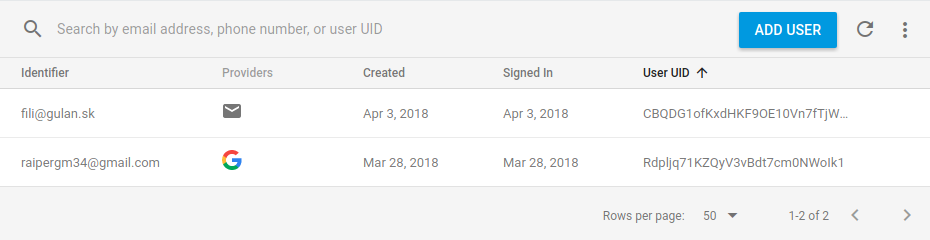
\includegraphics[scale=0.45]{fig/firebase.png}
  \caption{Ukážka záznamu vo Firebase Authentification}
  \label{fig:firebase}
\end{figure}

Liečenie, snímka rany, mierka sú potom typy dát, ktoré sú držané práve vo vlastnenom dátovom úložisku. Okrem týchto spomenutých kolekcií sa nachádza v databáze kolekcia  \textit{session}, ktorá predstavuje aktuálne sedenie užívateľa. To znamená, že táto kolekcia si drží základné informácie o aktuálne prihlásenom a v aplikácií pracujúcom užívateľovi. Dané sedenie si v sebe vždy drží token, získaný prihlásením pomocou Firebase, unikátny identifikátor užívateľa získaný znova z Firebase a ešte platformu, na ktorej je sedenie platné (buďto  \textit{core} pre internetový prehliadač,  \textit{core-electron} pre Electron desktop program, alebo  \textit{cordova-mobile-android} pre mobilnú Android aplikáciu). Výsledné kolekcie je možné vidieť v kóde.
\begin{lstlisting}[caption={Finálna štruktúra databáze},captionpos=b]
wound_database {
    scale: [
        {
            _id: 'scale-id-1',
            value: '1',
            unit: 'px',
            name: 'Scale 1',
            user: 'firebase-user-id-1',
        }
        ...
    ],
    session: [
        {
            _id: 'session-id-1',
            userId: 'firebase-user-id-1',
            platform: 'core',
        },
        ...
    ],
    therapy: [
        {
            _id: 'therapy-id-1',
            userId: 'firebase-user-id-1',
            name: 'Therapy 1',
            type: 'Decubit',
        },
        ...
    ],
    wound: [
        {
            _id: 'wound-id-1',
            therapy: 'therapy-id-1',
            user: 'firebase-user-id-1',
            originalLocation: '/home/filip/images/therapy-id-1.jpg'
            date: '154789',
            ...
        },
        ...
    ],
}
\end{lstlisting}
Kód obsahuje vždy iba pár nevyhnutných položiek, ktoré stačia na predstavu, ako je to v databáze uložené. O to, že sa v kolekcií nachádzajú ďalšie dokumenty daného typu informujú tri bodky. V tomto kóde je možné si všimnúť, ako nakoniec boli realizované vzťahy medzi jednotlivými entitami. Napríklad vzťah medzi  \textit{therapy} a  \textit{wound} je realizovaný pomocou odkazov, kedy  \textit{wound} obsahuje v sebe položku  \textit{therapy}, ktorá odkazuje na dané konkrétne liečenie podľa unikátneho identifikátoru tohoto liečenia. Vzťahy na základe referencií namiesto zanorovania štruktúr, ktoré NoSQL podporuje, boli zvolené kvôli tomu, že v podstate všetky ďalšie vzťahy sú iba vzťahy medzi entitou vo vlastnej databáze a používateľom vo Firebase Authentification úložisku a chcelo sa zachovať akýsi jednotný štandard práce s dátovými entitami.  MongoDB, ako aj iné databázy, umožňuje uložiť obrázky priamo do databáze. Pre intuitívnejšiu prácu s aplikačným serverovým rozhraním sa do databáze ale ukladajú iba cesty k súborom, ktoré sú uložené v priečinkoch na servery.

%%%%%%%%%%%%%%%%%%%%%%%%%%%%%%%%%%%%%%%%%%%%%%%%%%%%%%%%%%%%%%
\section{Implementácia serverového aplikačného rozhrania}
Aplikačné rozhranie REST nachádzajúce sa na strane serveru bolo postavené na rámci Flask a ďalších pomocných knižníc programovacieho jazyka Python. Celá programová realizácia tohoto rozhrania bola rozdelená do niekoľkých samostatných súborov a každý tento súbor predstavuje vlastne danú triedu zabezpečujúca konkrétnu sadu operácií. Realizácia obsahuje dokopy 6 súborov, z toho 1 súbor plniaci funkciu hlavnej funkcie, ktorá je mienená ako hlavný prístupový bod a 5 samostatných tried.
\begin{itemize}
\item Trieda \textit{Auth} v súbore \textit{auth.py} zabezpečuje iba jednu konkrétnu funkcionalitu a to overenie tokenu, teda či daný prichádzajúci token, ktorým sa preukazuje daný prihlásený užívateľ patrí naozaj k nejakému účtu vo Firebase Authentification.

\item Súbor \textit{database.py} obsahujúci triedu \textit{Database} zabezpečuje zase všetku prácu s MongoDB databázou za pomoci funkcií a metód knižnice pymongo. V tejto triede sa vytvára spojenie s databázou identifikovanou jej menom na danom servery a porte. V rámci tejto práce sa jedná o server s adresou \textit{127.0.0.1} teda \textit{localhost}, keďže aplikačné rozhranie a databáza sa nachádzajú na rovnakom stroji, port \textit{27017} a databázu \textit{wound\_database}. Okrem toho obsahuje metódy na prácu s dokumentami a kolekciámi tejto databáze.

\item Súbor \textit{httpStatusCode} obsahuje Hypertext Transfer Protokol stavové kódy serveru, ktoré sa využívajú pre zlepšenie čitateľnosti kódu. Sú v tejto triede uložené ako konštanty.

\item Trieda \textit{Pdf} uložená v súbore \textit{pdf.py} slúži na generovanie Portable Document Format súborov s dátami získaných z databáze. V triede sa nachádzajú 2 šablóny v HTML  formáte podľa ktorých sa generuje výsledný pdf súbor. Jedna šablóna je pre dáta o liečení a druhá pre dáta o rane. V pdf súbore liečenia sa nachádza okrem textových informácií ešte aj graf priebehu liečby, ktorý je najprv generovaný pomocou knižnice matplotlib a uložený ako obrázok. Tento obrázok sa následne vkladá do pdf suboru počas jeho tvorby. Tvorbu pdf súborov zabezpečuje knižnica pdfkit. Celý podrobný proces tvorby pdf súborov na strane serveru a prepojenie s klientskou stranou sa nachádza ďalej v kapitole.

\item Poslednou triedou, a to jednoznačne v rámci tohoto diplomového projektu aj najvýznamnejšou triedou, je trieda \textit{Vision}. Trieda je uložená znovu v rovnomennom súbore \textit{vision.py}. Zabezpečuje všetko okolo spracovania snímky rany, detekcie rany zobrazenej na snímke, detekcie mierky a vypočítania plochy rany na základe mierky a rany samotnej. Všetky tieto detekcie a výpočty sú realizované pomocou knižnice OpenCV. Spracovaniu snímky, detekcií a výpočtu plochy je ešte v tomto texte venovaný značný ďalší priestor, keďže ide o významnú časť práce.
\end{itemize}

Prístupovým bodom do aplikačného rozhrania, ktorý spracováva požiadavky klientov a následne im odpovedá je súbor \textit{main.py}. V tomto súbore sú definované všetky prístupové koncové adresy k zdrojom serveru a všetky možné metódy týchto adries. Pri požiadavke na adresu serveru bez akýchkoľvek ďalších ciest k zdroju pomocou metódy \textit{GET}  je vrátený reťazec \textit{“Wound detector API V1”}, ktorý slúži na overenie, či na danej doméne beží naimplementované aplikačné rozhranie. Pri požiadavke na adresu \textit{/static/priečinok/menosúboru} je vrátený nahraný súbor podľa svojho \textit{mena} nachádzajúci sa na servery v danom \textit{priečinku}. Adresa \textit{/auth/platforma} slúži na prihlasovanie a odhlasovanie užívateľa podľa zvolenej metódy na danej \textit{platforme}. Metódou \textit{POST} sa užívateľ do aplikácie prihlasuje, metódou \textit{DELETE} naopak odhlasuje. Ostatné adresy vo formáte \textit{/zdroj} slúžia na prístup k určenému zdroju a k manipulácií s týmto zdrojom na základe zvolenej metódy. \textit{GET} pre prístup k zdroju. \textit{POST} pre vytvorenie nového zdroju. Adresy vo formáte \textit{/zdroj/id} slúžia na prístup ku konkrétnemu zdroju identifikovanému pomocou unikátneho identifikátoru. Metódou \textit{GET} sa takýto zdroj získa, metódou \textit{PUT} modifikuje a metódou \textit{DELETE} odstráni. 


\subsection{Cross-Origin Ressource Sharing}
Odosielanie požiadaviek na server je limitované tzv. \textit{Same origin policy} a teda nie je možné prijímať odpovede na požiadavky z inej domény, ako je doména, z ktorej bolo požiadané. Túto veľmi známu limitáciu rieši \textit{Cross-origin resource sharing}, ďalej iba \textit{CORS}. CORS je vlastne mechanizmus, ktorý povoľuje zakázané zdroje na internetovej stránke, a tak aplikácie alebo internetové stránky môžu prijímať aj odpovede na požiadavky z inej domény, ako je doména, na ktorej sa aplikácia, alebo internetová stránka nachádza. Pre použitie musí nastať iba jednoduchá modifikácia hlavičiek v odpovedi serveru. Prehliadač musí posielať hlavičku \textit{Origin} nastavenú na aktuálnu doménu aplikácie, poprípade webovej stránky. Server musí posielať hlavičku \textit{Access-Control-Allow-Origin}, s hodnotou konkrétnej povolenej domény (domény aplikácie, alebo internetovej stránky), ktorá môže prijímať odpovede zo servera. Pre povolenie všetkých domén bez rozdielu sa používa *, čo je pre serverové rozhranie tejto práce chcené, keďže aplikácia bude bežať v rôznych zariadeniach a na rôznych platformách. Ďalej je možné ešte špecifikovať ďalšie nastavenia ako napríklad, ktoré \textit{HTTP} metódy budú povolené. Toto je zabezpečené hlavičkou \textit{Access-Control-Allow-Methods}, ale ani táto hlavička ani iné z rodiny \textit{Access-Control-Allow-*} nie sú v projekte využívané \cite{Hossain2015}. 

\textit{CORS} teda funguje v nasledujúcich jednoduchých krokoch:
\begin{enumerate}
\item \textit{CORS} požiadavku iniciuje klientská strana, aplikácia.
\item Prehliadač vloží do \textit{HTTP} požiadavky hlavičky, spolu s hlavičkou \textit{Origin}.
\item Server detekuje požiadavku, vytvorí odpoveď na túto požiadavku, vloží do nej \textit{HTTP} hlavičky spolu s hlavičkou \textit{Access-Control-Allow-Origin}, ktorá indikuje, že odpoveď je povolená na danej doméne a nakoniec túto odpoveď odošle prehliadaču.
\item Prehliadač detekuje, či je odpoveď na požiadavku povolená.
    \begin{enumerate}
    \item V prípade, že je požiadavka povolená prehliadač pošle dáta ďalej aplikácií alebo internetovej stránke.
    \item V prípade neexistencie hlavičiek v odpovedi, alebo neočakávania je odpoveď zamietnutá a klientská aplikácia si nemôže prečítať tieto dáta.
    \end{enumerate}
\end{enumerate}

\begin{figure}[h]
  \centering
  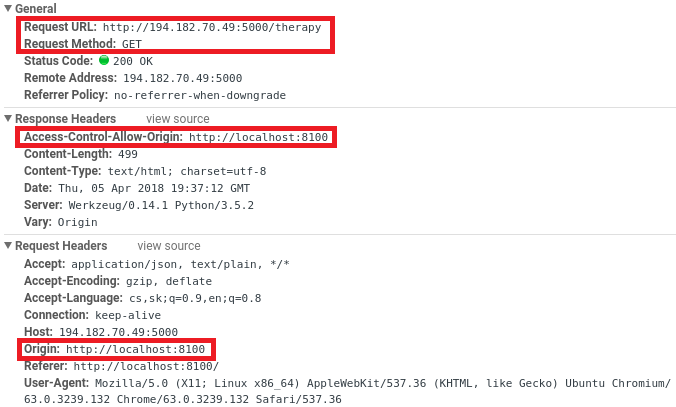
\includegraphics[scale=0.8]{fig/cors.png}
  \caption{Detail HTTP požiadavku a odpovede s hlavičkami \textit{CORS}}
  \label{fig:cors}
\end{figure}
Obrázok \ref{fig:cors} zobrazuje náhľad na požiadavku vykonanú na server a odpoveď, ktorú server vrátil. Tento obrázok bol získaný z Chrome developer tools konzole, ktorá je dostupná v internetových prehliadačoch Chrome, alebo Chromium. Na obrázku je vidieť, že sa vykonávala požiadavka na adresu \textit{http://194.182.70.49:5000/therapy} metódou \textit{GET} za účelom získania zoznamu liečení. Ďalej je možné vidieť, že do požiadavky boli vložené rôzne \textit{HTTP} hlavičky, medzi ktorými nechýba ani hlavička \textit{Origin}. Po tom, ako server spracoval požiadavku, odoslal odpoveď so štandardnými hlavičkami. Okrem štandardných hlavičiek server do odpovede vložil hlavičku \textit{Access-Control-Allow-Origin}. O povolenie mechanizmu \textit{CORS} sa v rámci tejto práce stará knižnica navrhnutá špeciálne pre Flask rámec, menom Flask-Cors.  Pre aktivovanie tejto knižnice stačí zavolať funkciu \textit{CORS(app)} a knižnica už sama do každej odpovede pridáva požadované \textit{CORS} hlavičky.

\subsection{Spracovanie snímkov}
TODO

%%%%%%%%%%%%%%%%%%%%%%%%%%%%%%%%%%%%%%%%%%%%%%%%%%%%%%%%%%%%%%
\section{Implementačné detaily}
Niektoré procesy sú vykonávané aj na strane klienta, to znamená v mobilnej, alebo desktopovej aplikácií, a aj na strane serveru v aplikačnom rozhraní. Medzi takéto procesy patrí napríklad prihlásenie užívateľa do aplikácie, získavanie snímkov, alebo generovanie PDF súborov. Všetky tieto procesy, ktoré sú vykonávané z časti na klientovi a z časti na servery sú bližšie popísané práve v tejto kapitole.

\subsection{Prihlasovanie}
Prihlasovanie v aplikácií patrí ku komplexnejším procesom v rámci programovej realizácie. Tento proces je z časti vykonávaný vo Firebase Authentification, z časti na aplikačnom serverovom rozhraní a z časti v klientskej aplikácií. Je mu z toho dôvodu venovaná samostatná kapitola obsahujúca aj dovysvetľujúci obrázok \ref{fig:login}.

Firebase vo svojej momentálnej implementácií nepodporuje v Electron, v NW.js alebo v iných desktopových aplikáciach prihlasovanie pomocou Google účtu. Vo fórach a Github problémoch všetko naznačuje tomu, že v budúcnosti bude možné aj tento typ prihlasovania. Momentálne však hlavne kvôli bezpečnosti toto umožnené nie je. Tento problém bol vyriešený tak, že v desktopovej Electron aplikácií sa namiesto prihlasovania Google účtom prihlasuje iba pomocou e-mailu a hesla. Je avšak nutné upozorniť, že užívateľ zaregistrovaný a prihlásený e-mailom a heslom sa v žiadnom prípade nezhoduje s užívateľom vytvoreným a prihláseným pomocou Google účtu. Užívateľ zaregistrovaný Google účtom \textit{novak@gmail.com}, nie je ten istý užívateľ ako \textit{novak@gmail.com} zaregistrovaný e-mailom a heslom. Firebase Authentification týchto užívateľov vidí ako 2 rôznych, keďže sa jedná o 2 úplne odlišné typy prihlásenia, pričom užívateľ prihlasovaný e-mailom a heslom sa do aplikácie v podstate normálne registruje a jeho heslo neodpovedá heslu Google účtu ale heslu zvolenému pri registrácií. Na obrázku \ref{fig:electron-app} je vidieť okno desktopovej verzie aplikácie zobrazujúce prihlasovanie pomocou e-mailu a hesla.
\begin{figure}[h]
  \centering
  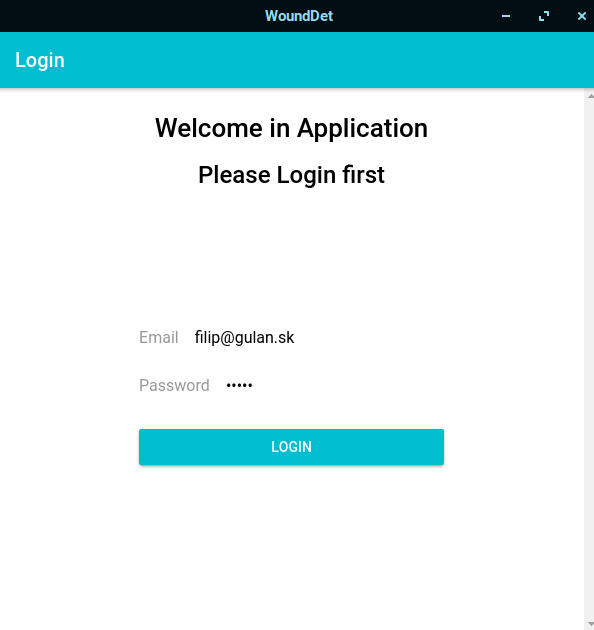
\includegraphics[scale=0.5]{fig/electron.png}
  \caption{Prihlasovacia obrazovka desktopovej verzie aplikácie}
  \label{fig:electron-app}
\end{figure}

Prihlasovanie začína na prihlasovacej obrazovke/stránke. V prípade, že sa jedná o mobilnú Android aplikáciu, prípadne internetovú aplikáciu, tak je ponúknuté prihlasovanie aj pomocou Google účtu aj pomocou e-mailu a hesla. V prípade, že sa jedná o desktopovú verziu aplikácie, tak sa tam nachádza iba formulár slúžiaci na prihlasovanie pomocou e-mailu a hesla. Ide síce o 2 v podstate odlišné metódy prihlásenia, avšak vďaka Firebase Authentification ich prihlasovací cyklus v rámci aplikácie prebieha absolútne rovnako. Jediná odlišnosť je v tom, keď sa užívateľ prihlasuje prvý krát do aplikácie pomocou Google účtu, tak Firebase vytvorí vo svojej databázy záznam automaticky. Naopak pri metóde prihlasovania pomocou e-mailu a hesla sa tento záznam musí najprv vytvoriť programovo, teda pri prvom prihlasovaní prebieha akási prvotná registrácia užívateľa, ktorú vykonáva samotná klientská aplikácia. Po stlačení tlačítka na prihlásenie Google účtom, alebo tlačítka na prihlásenia vo formulári, sa vykoná požiadavka na server Firebase Authentification, ktorá sa pokúsi užívateľa prihlásiť a v prípade úspechu vráti objekt užívateľa s ostatnými informáciami, ako je napríklad platný token. Získaný token sa následne odošle na serverové aplikačné rozhranie tejto práce na koncovú adresu \textit{/auth/platforma} metódou \textit{POST}, kde platforma predstavuje platformu zariadenia, z ktorého sa užívateľ pokúša prihlásiť. Pred vykonaním požiadavky sa ešte nastaví \textit{HTTP} hlavička \textit{Authorization} na hodnotu získaného tokena. Na servery je tento token overovaný, či sa jedná o platný token získaný z Firebase Authentification. Okrem samotného overenia je znovu získaný aj užívateľ, ktorému patrí tento token. V prípade, že je token úspešne overený, tak sa vytvorí v databázy v kolekcií \textit{session} záznam predstavujúci dané sedenie identifikované svojim unikátnym identifikátorom a obsahujúce Firebase Authentification token, unikátny identifikátor prihláseného užívateľa a platformu z ktorej prihlásenie nastalo. Po tom, ako je token overený a je vytvorený dokument kolekcie \textit{session}, tak je následne prihlásený užívateľ vrátený v odpovedi do aplikácie. Vrátený užívateľ sa následne uloží do poskytovateľa autentifikácie (\textit{auth.provider}) a tieto informácie sú zobrazené v hlavnom menu, konkrétne je zobrazené meno, priezvisko, e-mail a fotka užívateľa. Po tom, ako bol užívateľ prihlásený v obidvoch častiach, aj vo Firebase Authentification časti a aj v časti serverového aplikiačného rozhania, je možné vykonávať dotazy na server pre získanie súkromných dát, medzi ktoré patria doslova všetky požiadavky serveru, ako napríklad získanie zoznamu liečení, zoznamu rán a podobne. Všetky požiadavky po procese prihlásenia teda obsahujú \textit{HTTP} hlavičku \textit{Authorization} s hodnotou tokenu z Firebase Authentification. Po požiadaní serveru o zdroj sa na servery táto hlavička získa a porovnáva sa, či sa v databázy v kolekcií session nachádza takýto užívateľ. V prípade, že sa takýto užívateľ v kolekcií nenachádza, server vráti \textit{401 UNAUTHORIZED}. V opačnom, v kladnom prípade je užívateľ získaný z databázy a jeho identifikátor je ďalej používaný pre získavanie žiadúcich zdrojov. Celý tento proces je pre názornosť zobrazený na obrázku \ref{fig:login}. 
\begin{figure}[h]
  \centering
  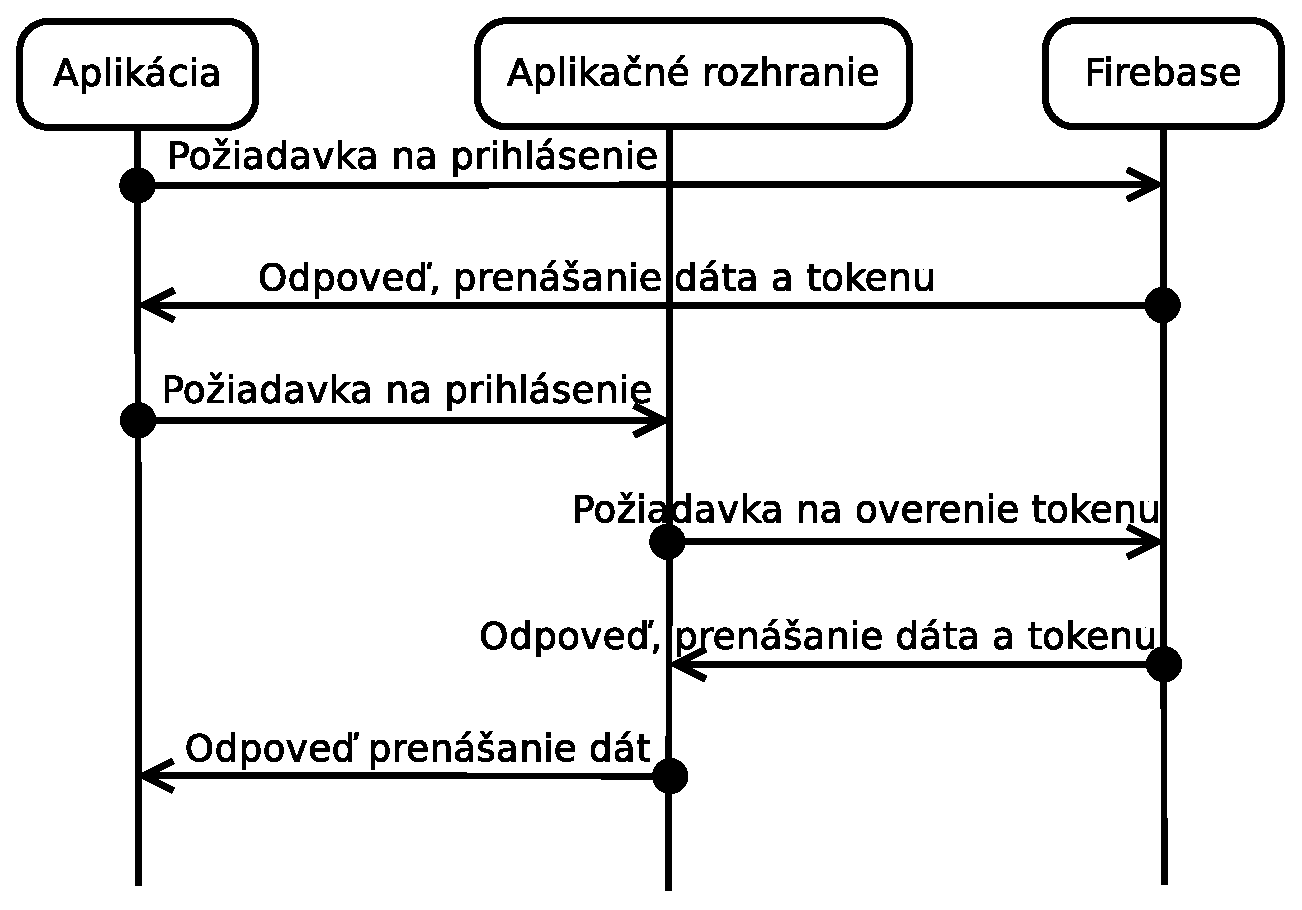
\includegraphics[scale=0.5]{fig/login.eps}
  \caption{Priebeh prihlasovania}
  \label{fig:login}
\end{figure}

\subsection{Získavanie snímkov}
Medzi najvýznamnejšie procesy práce patrí jednoznačne aj proces vyhotovovania snímkov. Tento proces prebieha z časti v aplikácií a z časti na aplikačnom servery. Proces začína na stránke detailu konkrétneho liečenia, kde si užívateľ zvolí v rozkladacom plávajúcom tlačítku, či chce použiť už hotové snímky z lokálneho úložiska svojho zariadenia, alebo chce ranu rovno zosnímať pomocou mobilnej počítačovej kamery, poprípade fotoaparátu. Ak si užívateľ vyberie prvú možnosť a zvolí si už existujúcu snímku z lokálneho úložiska, tak sa táto snímka predáva modálnemu oknu ukážky rany pomocou \textit{NavParams}. V druhom prípade sa iba prejde do rovnakého modálneho okna ale bez predania dát. V tomto modálnom okne sa v konštruktore detekuje, či boli predané nejaké dáta. V prípade existencie dát, sú tieto dáta zakódované do formátu \textit{Base64}\footnote{\textit{Base64} je kódovanie, alebo mechanizmus, ktorý povoľuje prenos binárnych dát cez média, ktoré umožňujú iba prenos textu. Vznikol kvôli potrebe pridávať do e-mailov obrázkový, video alebo iný binárny obsah. Kóduje vždy 3 oktety binárnych dát pomocou 4 \textit{ASCII} znakov. \cite{Menon13122008}} a spôsobom, aký je bežný aj napríklad pre formulárové dáta tejto aplikácie, je obrázok odoslaný na aplikačný server. V prípade, že sa dáta v do komponenty nepredali, tak sa v konštruktore aktivuje kamera a užívatel má tak možnosť zosnímať ranu priamo. Po vyhotovení sa snímka tejto rany znovu prekonvertuje do \textit{Base64} formátu a odošle na aplikačný server. Aplikačný server príjme požiadavku obsahujúcu takto zakódovaný obrázok, obrázok prekóduje naspäť do originálneho kódovania, vytvorí dočasný dokument v kolekcií \textit{wounds} a obrázok uloží do priečinku \textit{static/shoots} s menom \textit{identifikátoru} vytvoreného dočasného dokumentu v kolekcií \textit{wounds}. Tento obrázok sa následne spracuje a prebehnú všetky požadované výpočty. Po úspechu tejto operácie je v aplikácií zobrazený daný spracovaný obrázok, tak že HTML element \textit{img} obsahuje v atribúte \textit{src} hodnotu adresy, ktorá sprostredkováva obrázky uložené na servery (\textit{/static/shoots/wound-id.jpg}). Zobrazením obrázku je užívateľ vyzvaný, či sa daný obrázok použije ako finálna snímka rany, alebo chce proces opakovať a použiť, alebo vytvoriť inú snímku. V prípade nevyhovujúcej snímky, kedy napríklad bola rana nesprávne detekovaná kvôli svetelným alebo iným podmienkam, tak užívateľ zvolí možnosť opakovať proces a znovu sa aktivuje kamera, s tým že dočasný obrázok je zo serveru vymazaný. V prípad, že obrázok vyhovuje, prejde sa do modálneho okna editácie/vytvárania snímky, kde užívateľ je nútený vyplniť konečné informácie potrebné pre vytvorenie snímky. Povinnou položkou v tomto formulári je iba meno, ktoré je prednastavené na \textit{“Wound photo + aktuálny dátúm”} a položka mierky. Po vyplnení a odoslaní formulára je vytvorená konečne finálna snímka rany zobrazujúca sa v zozname snímok v detaile daného liečenia. Ak sa proces v ktoromkoľvek kroku preruší, tak je dočasný dokument z databáze spolu s dočasnou snímkou vymazaný.

\subsection{Generovanie PDF súborov}
Ďalším procesom, ktorý presahuje rozdelenie na proces aplikácie a proces serveru je generovanie súborov typu Portable Document Format s informáciami o danom liečení, alebo o danej konkrétnej rane. Generovanie je možné zahájiť na stránke detailu liečenia v kontextovom menu, alebo v kontextovom  menu na stránke detailu rany. Napriek tomu, že Javascript knižnice dokážu programovo vytvárať jednoduché PDF súbory, bola zvolená možnosť generovania týchto súborov na servery. Rozhodnutie bolo vykonané hlavne kvôli obmedzeniam vo finálnej Android aplikácií, kde aj po početných pokusoch sa nepodarilo takto generovaný súbor správne uložiť do zariadenia. PDF súbory sa teda generujú na servery. Proces generovania súboru iniciuje klientská aplikácia, alebo lepšie povedané užívateľ výberom možnosti generácie PDF v kontextovom menu. Po výbere tejto možnosti je úžívateľovi zobrazené okno načítania, ktoré je prítomné po celú dobu, až pokiaľ nie je súbor definitívne stiahnutý, alebo nenastala nejaká neočakávaná chyba. Následne je odoslaná na server požiadavka o generovanie súboru \textit{HTTP} metódou \textit{POST}. Server túto požiadavku príjme, získa informácie z databáze potrebné pre PDF súbor a pomocou knižnice PDFKit začne podľa HTML šablóny generovať samotný PDF súbor, ktorý uloží do priečinku \textit{static/pdfs}. V prípade, že PDF súbor má obsahovať aj graf, konkrétne PDF súbory liečení obsahujú grafy, tak sa najprv tento graf vygeneruje a uloží sa ako Portable Network Graphic obrázok do priečinku \textit{static/temp} odkiaľ sa potom použije v šablóne.  Po skončení operácie na servery je klientovi vrátený \textit{HTTP} statu kód \textit{200}. Týmto status kódom užívateľ vie, že PDF súbor je pripravený na stiahnutie. Sťahovanie samotného PDF súboru prebieha rozdielne pri Mobilnej a Desktopovej aplikácií. Pre stiahnutie súboru na platforme Android sa využíva natívny Cordova pluginu menom FileTransfer, ktorý súbor zo serveru stiahne a uloží do externého dátového priečinku, to je do priečinku \textit{Android/data/net.raiper34.wounddetector/files}. Užívateľ je o tomto úspechu informovaný pomocou upozorňovacieho okna, v ktorom je zobrazená cesta k súboru. Aj v prípade  desktopovej verzie nebolo možné stiahnuť súbor iba pomocou tradičných metód, ako napríklad pridanie atribútu \textit{download} pre kotvový element. Namiesto toho sa musela vykonať požiadavka na server metódou \textit{GET} a špecifikovať hlavička \textit{responseType} nastavená na hodnotu \textit{arrayBuffer}\footnote{ArrayBuffer objekt sa používa pre reprezentovanie všeobecnej vyrovnávacej pamäte surových binárnych dát s pevnou dĺžkou.\cite{lkToNI4tHykidWsV}}. Dáta, ktoré boli následne získané zo serveru sa potom pomocou  objektu \textit{Blob}\footnote{Blob objekt reprezentuje nemenné surové dáta, ktoré sú podobné súborovým dátam. Tieto dáta nemusia nutne reprezentovať natívny Javascript formát.\cite{m3Dxu36mfpc2MCxI}} a knižnice FileSaver uložili na užívateľom vybrané miesto. Keďže užívatel si sám volí, kde sa súbor uloží, tak o úspechu je informovaný obyčajnou \textit{Toast} komponentou so základnou hláškou úspechu.

\chapter{Testovanie a vyhodnocovanie}
\label{chap:testovanie-vyhodnocovanie}
Po naimplementovaní navrhnutého riešenia, ktoré bolo popísané v kapitole \ref{chap:implementacia}, nasledovalo testovanie a vyhodnocovanie, ktorému sa venuje práve táto kapitola.  Kapitola začína popisom testovania serverového aplikačného riešenia pomocou testovacieho rámca Tavern, pokračuje testovaním užívateľského rozhrania aplikácie a vyhodnocovaním naimplementovanej detekcie chronických rán. Na záver kapitoly sú zhrnuté ďalšie možné vylepšenia práce a je načrtnuté budúce smerovanie projektu. 

%%%%%%%%%%%%%%%%%%%%%%%%%%%%%%%%%%%%%%%%%%%%%%%%%%%%%%%%%%%%%%
\section{Testovanie serverového aplikačného rozhrania}
Testovanie aplikačného rozhrania prebiehalo už počas samotnej implementácie, kedy vždy po naprogramovaní nejakej sady koncových adries, boli napísané aj testy na overenie funkcionality týchto adries. Testovanie prebiehalo pomocou Python testovacieho rámca Tavern, ktorý je voľne dostupný pod licenciou MIT. Tavern je plugin pre Pytest, nástroj príkazovej riadky a aj Pythonova knižnica v jednom určená pre testovanie aplikačných rozhraní založených nielen na RESTe. Používa syntax založenú na YAML, ktorá je veľmi flexibilná a jednoduchá. Okrem RESTful aplikačných rozhraní dokáže testovať aj rozhrania založené na MQTT. Veľká výhoda Tavern je, že môže byť veľmi jednoducho použitý v hocijakom continous integration procese. \cite{AXUaooptJGOSpUrX} 

Testy vytvorené pre Tavern sú teda definované v YAML súboroch, ktoré predstavujú danú testovaciu sadu. Táto sada je vždy definovaná svojím menom (\textit{test\_name}) a jednotlivými krokmi samotného testu (\textit{stages}).  Každý jeden krok predstavuje samostatné dotazovanie sa na server a volanie serverovej funkcie. Kroky sa skladajú z mena kroku (\textit{name}), z požiadavky (\textit{request}), ktorá sa vykonáva a z odpovede (\textit{response}), ktorá sa kontroluje. V požiadavke je možné definovať všetky nastavenia, ako url adresy serveru (\textit{url}), na ktorý sa bude posielať požiadavka, metódu, ktorá sa bude vykonávať (\textit{method}), dáta vo formáte json, ktoré sa na server budú odosielať (\textit{json}) a prípadne ďalšie hlavičky (\textit{headers}), ktoré sú v požiadavke prítomné (v tomto prípade je prítomná iba hlavička \textit{Authorization}). Správnosť odpovede, ktorá sa potom vyhodnocuje je overovaná podľa vráteného stavového kódu (\textit{status\_code}) a dát obsiahnutých v tele (\textit{body}), poprípade iných položiek, ktoré ale v prípade tejto práce nie sú potrebné. Štruktúru takéhoto kroku testu je možné vidieť pre predstavu v kóde. 
\begin{lstlisting}[caption={Ukážka testovacieho kroku.},captionpos=b]
...
- name: Get scale list after update
    request:
      url: "{env_host:s}/scale"
      method: GET
      headers:
        Authorization: "{firebase_token:s}"
    response:
      status_code: 200
      body:
        - name: Scale
          unit: px
          value: 10
          user: "{firebase_user:s}"
          _id:
            \$oid: "{scale_id:s}"
...
\end{lstlisting}
Testy sú spúšťané pomocou nástroju príkazového riadku Tavern-CI. Testy tejto práce boli rozdelené do 2 súborov, a to na prípady, ktoré môžu nastať pri každodennom používaní aplikácie (\textit{valid.tavern.yaml}) a na prípady, ktoré by mohli nastať iba v prípade nejakej neočakávanej chyby, alebo pri pokuse o hackovanie aplikácie (\textit{invalid.tavern.yaml}). Súbor \textit{enviroment.yaml} slúži na uchovávanie premenných, ktoré sa používajú a sú vkladané do obidvoch testov. Ide o premennú kľúča k Firebase Authentification, e-mailu a hesla k účtu testovacieho užívateľa a koreňovú adresu serveru aplikačného rozhrania. Kroky testu sa vyhodnocujú postupne a v prípade, že sa nevyhodnotí správne jeden krok, tak vyhodnocovanie ďalších krokov je zrušené a užívateľ je o tejto skutočnosti informovaný. Po otestovaní finálnej podoby aplikačného serverového rozhrania, kedy všetky testy dopadli úspešne, bolo toto rozhranie považované za stabilné a fungujúce správne. 

%%%%%%%%%%%%%%%%%%%%%%%%%%%%%%%%%%%%%%%%%%%%%%%%%%%%%%%%%%%%%%
\section{Vyhodnocovanie detekcie chronickej rany}
Vyhodnocovanie a testovanie poloautomatickej detekcie bolo vykonávané na snímkoch chronických rán, ktoré poskytla Fakultná nemocnica Brno. Ide o snímky vytvorené pomocou bežného mobilného fotoaparátu, ktorý nebol ničím špeciálny a nachádza sa takmer v každom modernom mobilnom zariadení. Získavanie snímok neprebiehalo za prítomnosti žiadnych špeciálnych predpripravených podmienok. Snímky sú rôznej kvality a zachycujú rôzne chronické rany v rôznych štádiách, od rán, ktoré sa skoro neprejavili, až po rany, ktoré už boli v pokročilom štádií a značne komplikované ako na liečbu, tak aj na samotnú detekciu. Snímky boli získavané nemocnicou približne od polovice januára 2018 do polovice mája 2018 a takto bolo získaných 40 snímok zo 14 unikátnych defektov (v rovnakom čase bol ten istý defekt zachytený niekoľkokrát). Z týchto 14 defektov sa avšak nejednalo vždy o chronické rany, ale objavila sa aj snímka stareckých škvŕn, alebo jedno približne 60 ročné materské znamienko. Unikátnych chronických rán bolo teda dokopy 12 a z toho 10 bolo použitých pre vyhodnocovanie. Všetky unikátne rany boli autorom práce anotované za pomoci externého konzultanta tejto práce.

Výskumy, ktoré sa zaoberali detekciou chronických rán, alebo príbuzných defektov a boli behom práce na tomto projekte preštudované, boli vykonávané pod určitými kontrolovanými podmienkami, ako napríklad špeciálne nasvietenie rany a podobne (štúdie \cite{4353723}, \cite{6461344} a \cite{6399754}). Detekcia a analýza iných rán zase prebiehala iba na ručne predspracovaných snímkach, napríklad bez pozadia, alebo snímkach, ktoré obsahovali iba samotnú ranu (štúdie \cite{5286322} a \cite{6306219}). Iné štúdie ako \cite{6172044} alebo \cite{6392633} sa zase zamerali iba na určitý špecifický typ chronickej rany. Všetky tieto štúdie boli overované na dátovej sade obsahujúcej od 5 v \cite{6172044} do 113 snímkov v \cite{5286322}. Ich presnosť detekcie za týchto, dá sa povedať zjednodušených podmienok, dosahovala presnosť od 56,4\% v \cite{4353723} do 98\% v \cite{6306219}. Dá sa ale predpokladať, že takéto podmienky pri získavaní snímok pomocou mobilného zariadenia v bežnej lekárskej praxi nastať nemôžu, alebo iba veľmi ťažko. Sťažením tohoto projektu oproti spomenutým štúdiám bolo avšak to, že snímky neboli získavané behom žiadnych kontrolovaných podmienok, neboli ručne predspracované a taktiež kvôli nedostatku testovacieho materiálu bola práca zameraná na všetky typy chronických rán, nie iba na niektorých špecifických. 

Samotné vyhodnocovanie a testovanie bolo vykonávané tak, že testovacie snímky boli manuálne ohraničené externým konzultantom z nemocnice pomocou špeciálne vytvorenej webovej aplikácie pre tieto účely, ktorú je možné vidieť na obrázku \ref{fig:anotator} a tak vznikli akési predlohy na porovnávanie a vyhodnotenie poloautomatickej detekcie. 
\begin{figure}[h]
  \centering
  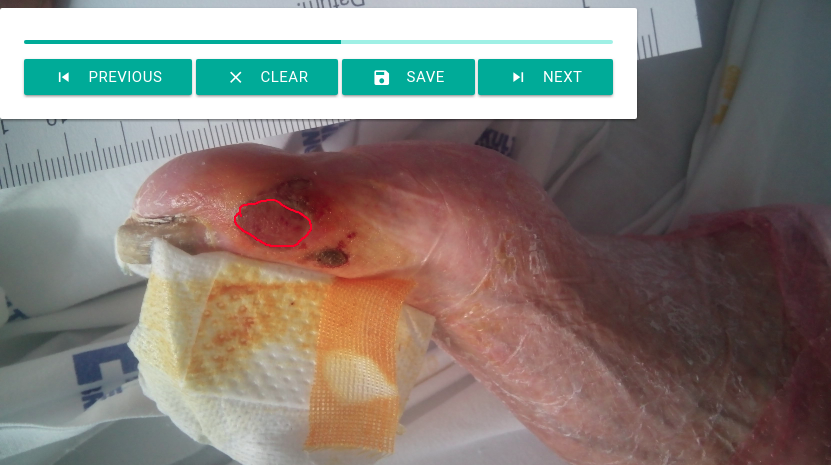
\includegraphics[scale=0.5]{fig/anotator.png}
  \caption{Webová aplikácia na ohraničovanie snímok konzultantom.}
  \label{fig:anotator}
\end{figure}
Je nutné podotknúť, že chronické rany sú veľmi zložité a keď sa stretne viacero špecialistov, tak môžu mať rozdielny názor na to, čo ešte patrí do priestoru rany a čo už rana nieje. Je teda nutné pri detekcií a aj tvorbe predlohy a porovnávaní s ňou vždy rátať s určitou dávkou subjektivity. Rany na snímkach boli potom detekované pomocou poloautomatickej metódy detekcie. Po detekcií boli hodnoty vypočítaného obsahu rany a očakávaného obsahu v pixeloch navzájom porovnávané. Výsledky je možné vidieť v tabuľke \ref{tab:result}, kde je vždy uvedené číslo rany, ktoré odpovedá menu súboru z priečinku \textit{shots/eval} nachádzajúceho sa na priloženom nosiči. Úspešnosť detekcie je vždy vyjadrená číselne v pixeloch a v percentách. Okrem úspešnosti detekcie je prítomný aj stĺpec, ktorý hovorí, koľko pixelov na obrázku bolo klasifikovaných nesprávne ako pixel chronickej rany. 
\begin{table}[h]
\centering
\label{tab:result}
\begin{tabular}{|l|l|l|l|l|}
\hline
Rana & Detekované & Očakávané & Správne detekované & Nesprávne detekované \\ \hline
1    & 6280px               & 13820px           & 6213px (44.96\%)    & 67px         \\ \hline
2    & 0px                  & 261px             & 0px (0.00\%)        & 0px          \\ \hline
3    & 1108px               & 10296px           & 1041px (10.11\%)    & 67px         \\ \hline
4    & 10484px              & 2244px            & 2244px (100.00\%)   & 8240px     \\ \hline
5    & 7499px               & 8285px            & 5424px (65.47\%)    & 2075px      \\ \hline
6    & 3026px               & 2495px            & 2038px (81.68\%)    & 988px       \\ \hline
7    & 46712px              & 34051px           & 34046px (99.99\%)   & 12666px     \\ \hline
8    & 6307px               & 7182px            & 6161px (85.78\%)    & 146px        \\ \hline
9    & 23917px              & 2301px            & 2301px (100.00\%)   & 21616px    \\ \hline
10   & 5509px               & 6560px            & 5022px (76.55\%)    & 487px        \\ \hline
\end{tabular}
\caption{Výsledky vyhodnocovania poloautomatickej detekcie}
\end{table}
V tabuľke výsledkov je možné si všimnúť, že výsledné hodnoty boli rôzne, tak ako jednotlivé rany. Behom práce bolo navrhnuté, aby sa projekt zameral len na určitý druh rán v určitom štádií, vzhľadom na to, aké až príliš rozdielne boli jednotlivé rany na snímkach. Bohužiaľ ale behom pol roka nebolo možné získať taký dostatočný počet snímkov, aby sa bolo možné užšie zameranie. Z obrázkov je jasné, že čo rana to v podstate iný druh v inom štádií a preto boli v rámci implementácie zvolené postupy také aké boli, teda okrem poloautomatickej detekcie algoritmom Region Growing bol pridaný aj manuálny mód ohraničenia rany. Z tabuľky je možné si všimnúť hodnoty úspešnosti detekcie, ktoré sú presne 100\%. Rany, ktoré majú takúto úspešnosť boli síce detekované celé, avšak do okolia rany bol zahrnutý aj predstupeň pred samotným defektom. Takúto ranu je možné vidieť na obrázkoch \ref{fig:w4} a \ref{fig:w4d}. Naopak veľmi dobre bola detekovaná rana, ktorá bola jasne iná ako okolitá pokožka a to tak, že aj lajk by dokázal ranu ohraničiť. Ranu je možné vidieť na obrázkoch \ref{fig:w8} a \ref{fig:w8d}.

%%%%%%%%%%%%%%%%%%%%%%%%%%%%%%%%%%%%%%%%%%%%%%%%%%%%%%%%%%%%%%
\section{Ďalšie smerovanie projektu}
Ako je možné zistiť podľa výsledkov, tak poloautomatická detekcia funguje rôzne na rôznych snímkach. Zatiaľ čo funguje na ranách, ktoré sú farebne dobre oddelené od okolitej kože, tak podstatne viac zlyháva na ranách, ktoré sú menej výrazné, alebo sú pomerne komplikované. Avšak, aby boli tieto tvrdenia potvrdené, je nutné urobiť ďalšiu a oveľa väčšiu sadu snímkov, a keďže behom 5 mesačného obdobia bolo bolo zaznamenaných 12 unikátnych defektov, typu chronická rana, tak tento proces bude nezanedbateľne časovo náročný. Z toho dôvodu nie je úplne overená funkčnosť poloautomatickej detekcie. Aplikácia však môže byť využívaná, tak, že sa bude používať poloautomatická detekcia na pomerne jednoduchších a farebne výraznejších ranách, a na zložitejších ranách bude využívaná manuálna detekcia pomocou ohraničenia rany prstom/myšou. Okrem toho, že poloautomatická detekcia bola testovaná na chronických ranách, tak bola testovaná aj na pár snímkach hematómov a jednom výraznom znamienku, ktoré nemocnica taktiež poskytla. Ako je vidieť na obrázkoch \label{fig:w2} a \label{fig:w3}, tak aplikácia môže byť použitá aj na takéto prípady. Poprípade sa môže algoritmus ľahko upraviť, aby mohli byť detekované všetky tieto prípady, keďže hematómy sú v porovnaní s chronickými ranami oveľa menej rozmanité a teda viac farebne navzájom podobné.
\begin{figure}[h]
   \begin{minipage}{0.4\textwidth}
     \centering
     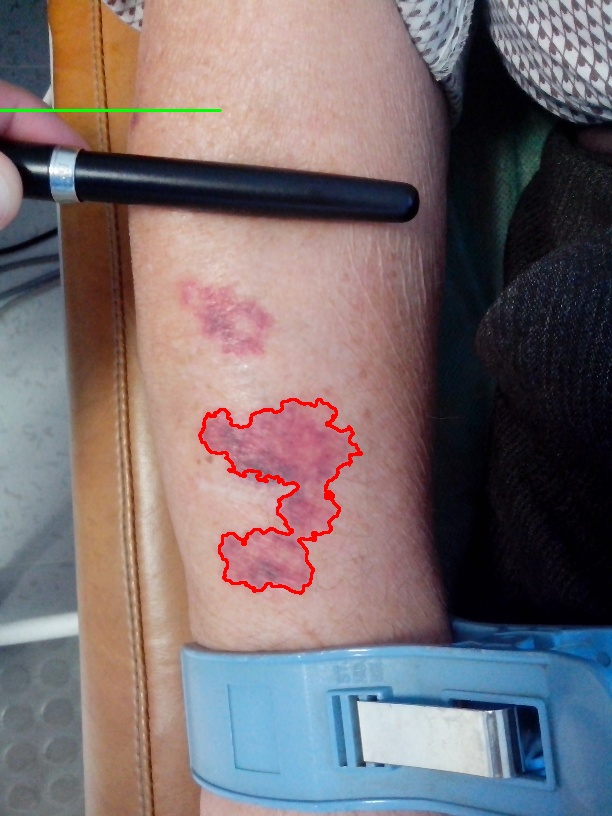
\includegraphics[scale=0.35]{fig/2o.jpeg}
      \caption{Detekcia hematómu.}
      \label{fig:w2}
   \end{minipage}\hfill
   \begin{minipage}{0.4\textwidth}
     \centering
     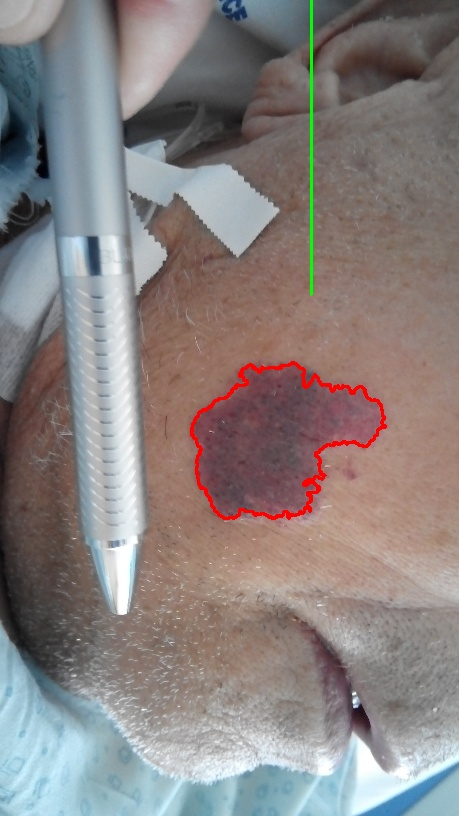
\includegraphics[scale=0.35]{fig/3o.jpeg}
      \caption{Detekcia znamienka.}
      \label{fig:w3}
   \end{minipage}
\end{figure}

\begin{figure}[h]
   \begin{minipage}{0.48\textwidth}
     \centering
     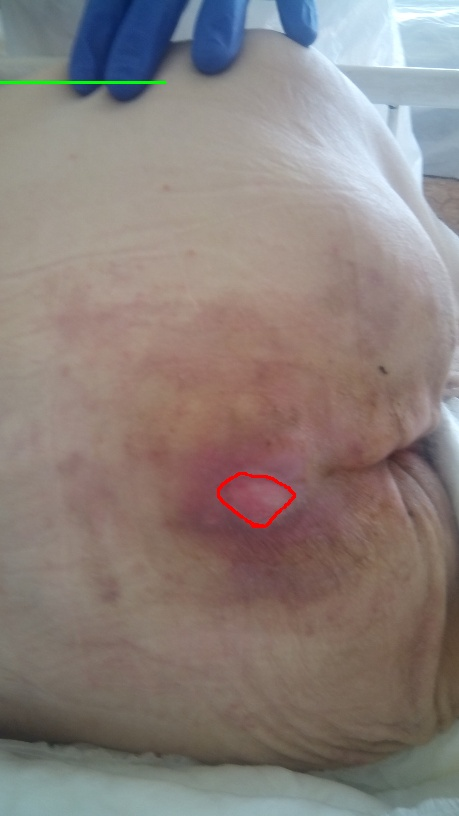
\includegraphics[scale=0.35]{fig/4m.jpeg}
      \caption{Rana 4 - manuálna detekcia, očakávaná.}
      \label{fig:w4}
   \end{minipage}\hfill
   \begin{minipage}{0.48\textwidth}
     \centering
     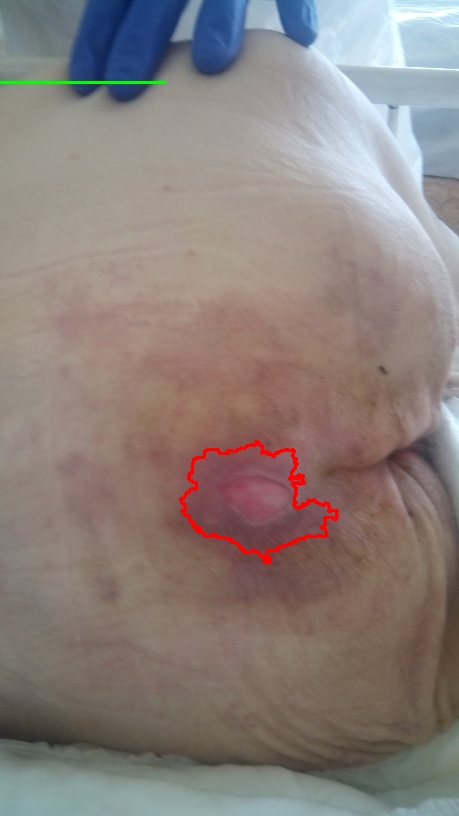
\includegraphics[scale=0.35]{fig/4a.jpeg}
      \caption{Rana 4 - automatická detekcia.}
      \label{fig:w4d}
   \end{minipage}
   \break \break \break
   \begin{minipage}{0.48\textwidth}
     \centering
     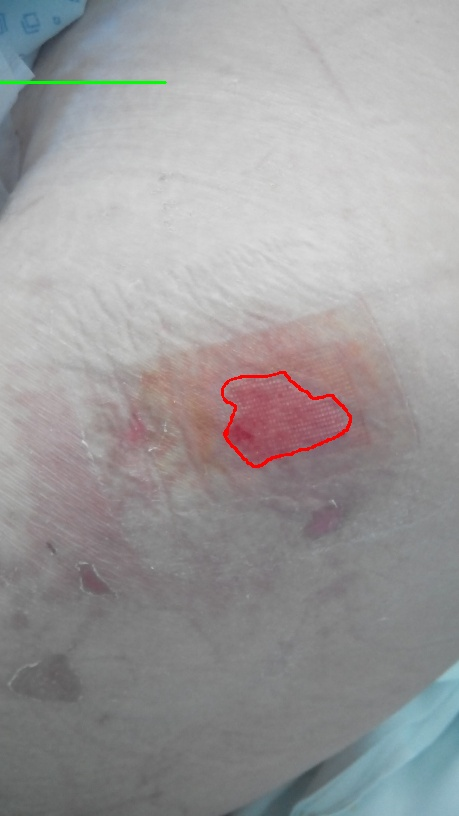
\includegraphics[scale=0.35]{fig/8m.jpeg}
      \caption{Rana 8 - manuálna detekcia, očakávaná.}
      \label{fig:w8}
   \end{minipage}\hfill
   \begin{minipage}{0.48\textwidth}
     \centering
     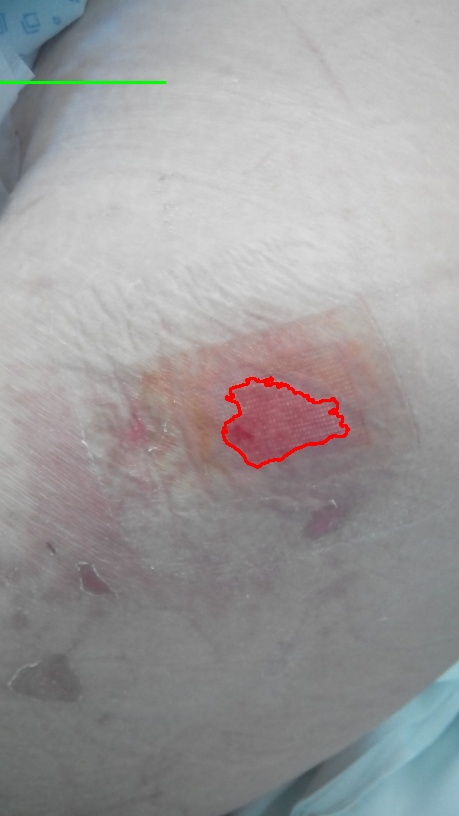
\includegraphics[scale=0.35]{fig/8a.jpeg}
      \caption{Rana 8 - automatická detekcia.}
      \label{fig:w8d}
   \end{minipage}
\end{figure}

\chapter{Záver}
Cieľom diplomovej práce bolo vytvorenie aplikácie pre zariadenia s operačným systémom Android a zariadenia s operačným systémom Windows pre detekciu, lokalizáciu a určenie plochy chronických rán. Táto aplikácia má slúžiť zdravotným sestrám, doktorom a ošetrovateľom ako pomoc pri vyhodnocovaní a sledovaní chronickej rany počas trvania liečby. Aplikácia je postavená na programovacom jazyku Typescript, hybridnom aplikačnom rámci Ionic a Electron. Detekcia chronickej rany prebieha na strane servera, kde sa využíva programovací jazyk Python, pre RESTful aplikačné rozhranie aplikačný rámec Flask a pre spracovanie obrazu knižnica OpenCV. Dáta sa ukladajú do NoSQL databáze MongoDB.

Práca na začiatku začínala kapitolou \ref{chap:teoreticky-rozbor}, ktorá sa venovala teoretickému rozboru a obsahuje informácie potrebné k základnému pochopeniu problematiky chronických rán. Ďalšia kapitola \ref{chap:analyza-navrh-riesenia} sa zaoberala analýzou a návrhom samotnej mobilnej aplikácie a jej serverových súčastí. Konkrétne popisovala návrh grafického užívateľského rozhrania, ale aj návrh aplikačného rozhrania REST a výber vhodných technologických prostriedkov. Hneď potom nasleduje kapitola \ref{chap:pouzite-techologie}, ktorá rozoberala technológie, ktoré boli potrebné pri vývoji aplikácie a jej súčastí. V poradí ďalšou a určite najvýznamnejšou kapitolou je kapitola \ref{chap:implementacia}, ktorá pojednávala o samotnej implementácií. Celá práca je ukončená kapitolou \ref{chap:testovanie-vyhodnocovanie} o testovaní a vyhodnocovaní implementovaného riešenia a sú navrhnuté ďalšie kroky a smerovanie práce.

Finálna Android a Windows aplikácia, ktorá vznikla v rámci tejto diplomovej práce dokáže detekovať, lokalizovať a určiť plochu zosnímanej chronickej rany. Aplikácia detekuje tieto rany poloautomaticky výberom bodu vo vnútri rany za pomoci Region Growing algoritmu nad RYKW pravdepodobnostnou mapou, alebo v prípade zložitejších chronických rán, kedy poloautomatická detekcia výrazne zlyháva je možné použiť manuálnu detekciu pomocou ohraničenia plochy rany pomocou prsta, alebo myši. Výpočet reálnej plochy rany je potom zabezpečený pomocou užívateľom zvolenej mierky, kedy sa vždy jeden pixel plochy prevádza do nejakej miery reálneho sveta. Aplikácia je teda použiteľná do určitej miery v klinickej praxi, avšak mala by byť ešte ďalej testovaná a vylepšovaná, poprípade by sa mala užšie zamerať na niektoré špecifické typy rán v konkrétnom štádií. Aplikácia ďalej môže byť ešte rozšírená tak, aby bola schopná detekovať rôzne iné defekty kože. Takýmito príkladmi môžu byť napríklad hematómy, alebo materské znamienka.

 % viz. obsah.tex / see obsah.tex

  % Pouzita literatura / Bibliography
  % ----------------------------------------------
\ifslovak
  \makeatletter
  \def\@openbib@code{\addcontentsline{toc}{chapter}{Literatúra}}
  \makeatother
  \bibliographystyle{bib-styles/czechiso}
\else
  \ifczech
    \makeatletter
    \def\@openbib@code{\addcontentsline{toc}{chapter}{Literatura}}
    \makeatother
    \bibliographystyle{bib-styles/czechiso}
  \else 
    \makeatletter
    \def\@openbib@code{\addcontentsline{toc}{chapter}{Bibliography}}
    \makeatother
    \bibliographystyle{bib-styles/englishiso}
  %  \bibliographystyle{alpha}
  \fi
\fi
  \begin{flushleft}
  \bibliography{citacie}
  \end{flushleft}

  % vynechani stranky v oboustrannem rezimu
  % Skip the page in the two-sided mode
  \iftwoside
    \cleardoublepage
  \fi

  % Prilohy / Appendices
  % ---------------------------------------------
  \appendix
\ifczech
  \renewcommand{\appendixpagename}{Přílohy}
  \renewcommand{\appendixtocname}{Přílohy}
  \renewcommand{\appendixname}{Příloha}
\fi
\ifslovak
  \renewcommand{\appendixpagename}{Prílohy}
  \renewcommand{\appendixtocname}{Prílohy}
  \renewcommand{\appendixname}{Príloha}
\fi
%  \appendixpage

% vynechani stranky v oboustrannem rezimu
% Skip the page in the two-sided mode
%\iftwoside
%  \cleardoublepage
%\fi
  
\ifslovak
%  \section*{Zoznam príloh}
%  \addcontentsline{toc}{section}{Zoznam príloh}
\else
  \ifczech
%    \section*{Seznam příloh}
%    \addcontentsline{toc}{section}{Seznam příloh}
  \else
%    \section*{List of Appendices}
%    \addcontentsline{toc}{section}{List of Appendices}
  \fi
\fi
  \startcontents[chapters]
  \setlength{\parskip}{0pt}
  % seznam příloh / list of appendices
  % \printcontents[chapters]{l}{0}{\setcounter{tocdepth}{2}}
  
  \ifODSAZ
    \setlength{\parskip}{0.5\bigskipamount}
  \else
    \setlength{\parskip}{0pt}
  \fi
  
  % vynechani stranky v oboustrannem rezimu
  \iftwoside
    \cleardoublepage
  \fi
  \chapter{Obsah CD}
\label{pr:cd}
Adresárová štruktúra CD
\begin{itemize}
\item \textit{src} - Zdrojové súbory
    \begin{itemize}
    \item \textit{app} - zdrojové súbory aplikácie
    \item \textit{api} - zdrojové súbory serverového aplikačného rozhrania
    \item \textit{db} - snímok Mongodb databéze
    \item \textit{shots} - testovacie snímky
    \item \textit{demo} - spustiteľné súbory (apk pre android a exe pre windows)
    \end{itemize}
\item \textit{text} - Text práce
\end{itemize}
 % viz. prilohy.tex / see prilohy.tex
\end{document}
